%%%%%%%%%%%%%%%%%%%%%%%%%%%%%%%%%%%%%%%%%%%%%%%%%%%%%%%%%%%

\chapter{Modello del sistema - gruppo 6}
\label{ref:modSistemaGruppo6}

%%% Il gruppo 6 scriverà il suo modello del sistema. Esso dovrà includere: attori, casi d'uso (descrizione e tabella), scenari, diagrammi dei casi d'uso, diagrammi di sequenza, diagramma delle attività, screen mockups della funzionalità %%%

\section{Attori}
Descrivere gli attori che partecipano ai seguenti caso d'uso.

%%%%%%%%%%%%%%%PER QUANTO RIGUARDA IL NOSTRO ATTORE STUDENTE, VERRà INTEGRATO CON QUELLO DI TUTTI FACENDO UNA REF AD UNA LABEL
%N.B.:
%Per quanto riguarda la funzionalità chat \ref{nome-label} l'attore %studente ha in aggiunta le seguenti caratteristiche: ...

\section{Scenari}
Inserire qui gli scenari che sono un'istanza dei casi d'uso: gli scenari danno dei valori al flusso degli eventi dei casi d'uso. Esempio di caso d'uso "visualizza libretto": l'utente Antonio - che ha effettuato il login con username "Antonio" e password "antonioilmigliore" - accede alla sezione "libretto" e visualizza gli esami sostenuti Programmazione e Inglese con le votazioni rispettive di 25 e 30.

\section{Casi d'uso}
Per ogni caso d'uso inserire descrizione e tabella. Se il tuo caso d'uso prevede più attori di quelli che sono nella tabella sottostante di esempio, aggiungi una colonna nella sezione flusso degli eventi!

\paragraph{Caso d'uso 1 (sostituire con nome caso d'uso) \\} 

%%%%%%%%%%%%%% METTERE LABEL AI NOSTRI CASI D'USO
%\label{nome-label}

Lorem ipsum dolor sit amet... (sostituire con descrizione caso d'uso)

\begin{table}
%\normalsize % Dimensione testo normale
\small % Dimensione testo piccola
%\footnotesize % Dimensione testo piccolissima
%\scriptsize % Dimensione del testo ulteriormente più piccola
%\caption{} % Didascalia tabella
%\label{} % Etichetta per riferimenti incrociati
\begin{tabular}{| p{\useCaseLeft} | p{\useCaseNum} | p{\useCaseTwoCol} | p{\useCaseTwoCol} |}
	\hline
	\textbf{Nome caso d'uso} & \multicolumn{3}{p{\useCaseMulticol} |}{\textbf{Login}} \\
	\hline
	\textbf{Attori partecipanti} & \multicolumn{3}{p{\useCaseMulticol} |}{Inizializzato da \textbf{Utente}.} \\
	\hline
	\textbf{Condizioni d'ingresso} & \multicolumn{3}{p{\useCaseMulticol} |}{L'utente ha cliccato sul bottone di login.} \\
	\hline
	\textbf{Flusso degli eventi} & \textbf{\#} & \textbf{Utente} & \textbf{Sistema} \\
	\hline
	\textbf{} & \textbf{1} & \textbf{} & Propone una schermata per l'inserimento dei dati necessari per il login, e-mail e password dell'utente \\
	\hline
	\textbf{} & \textbf{2} & Inserisce i dati e sottomette la richiesta & \textbf{} \\
	\hline
	\textbf{} & \textbf{3} & \textbf{} & Controlla che siano stati inseriti entrambi i campi e avvia le operazioni di visualizzazione \\
	\hline
	\textbf{Eccezioni} & \multicolumn{3}{p{\useCaseMulticol} |}{3.1 Uno o entrambi i campi sono vuoti.\newline 3.2 Le credenziali inserite non sono valide (una o entrambe).} \\
	\hline
	\textbf{Condizioni d'uscita} & \multicolumn{3}{p{\useCaseMulticol} |}{Il sistema completa la login e dà accesso all'app o, in caso contrario, visualizza un messaggio di errore se non sono stati inseriti tutti i dati obbligatori, se le credenziali non sono corrette o se si verifica un insuccesso dell'operazione.} \\
	\hline
\end{tabular}
\end{table}

\section{Diagramma dei casi d'uso}

Inserire immagine del diagramma. Le immagini vanno caricate nella cartella imgs, va inserito il path corrispondente (nomefile.estensione) dopo il tag includegraphics e va cambiata la descrizione dell'immagine (caption) con un'etichetta opportuna. Sostituire l'immagine file-comuni-ai-gruppi/useCaseEsempio.png con quella desiderata.

\begin{figure}
	\centering
	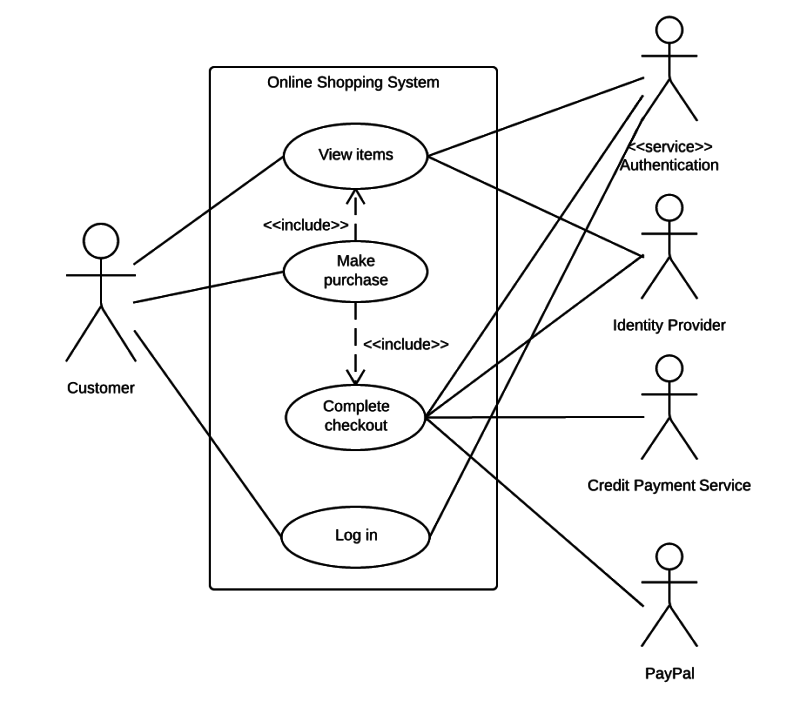
\includegraphics[height=3in]{imgs/file-comuni-ai-gruppi/useCaseEsempio.png}
	\caption{Inserire descrizione}
	\label{fig:prova}
\end{figure}

\section{Diagramma di sequenza}
Inserire immagine del diagramma. Le immagini vanno caricate nella cartella imgs, va inserito il path corrispondente (nomefile.estensione) dopo il tag includegraphics e va cambiata la descrizione dell'immagine (caption) con un'etichetta opportuna. Sostituire l'immagine file-comuni-ai-gruppi/useCaseEsempio.png con quella desiderata.

\begin{figure}
	\centering
	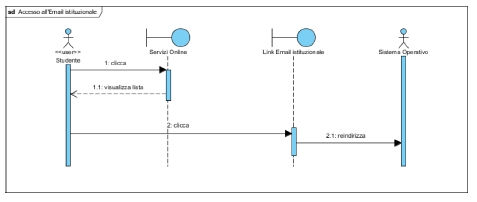
\includegraphics[height=3in,width=5in]{imgs/file-comuni-ai-gruppi/SequenceDgEsempio.png}
	\caption{Inserire descrizione}
	\label{fig:prova}
\end{figure}

\section{Diagramma delle attività}
%%% START activities chat studenti %%%
\begin{figure}
\subsection{Activities relative alla chat dell'App Studenti}
	\centering
	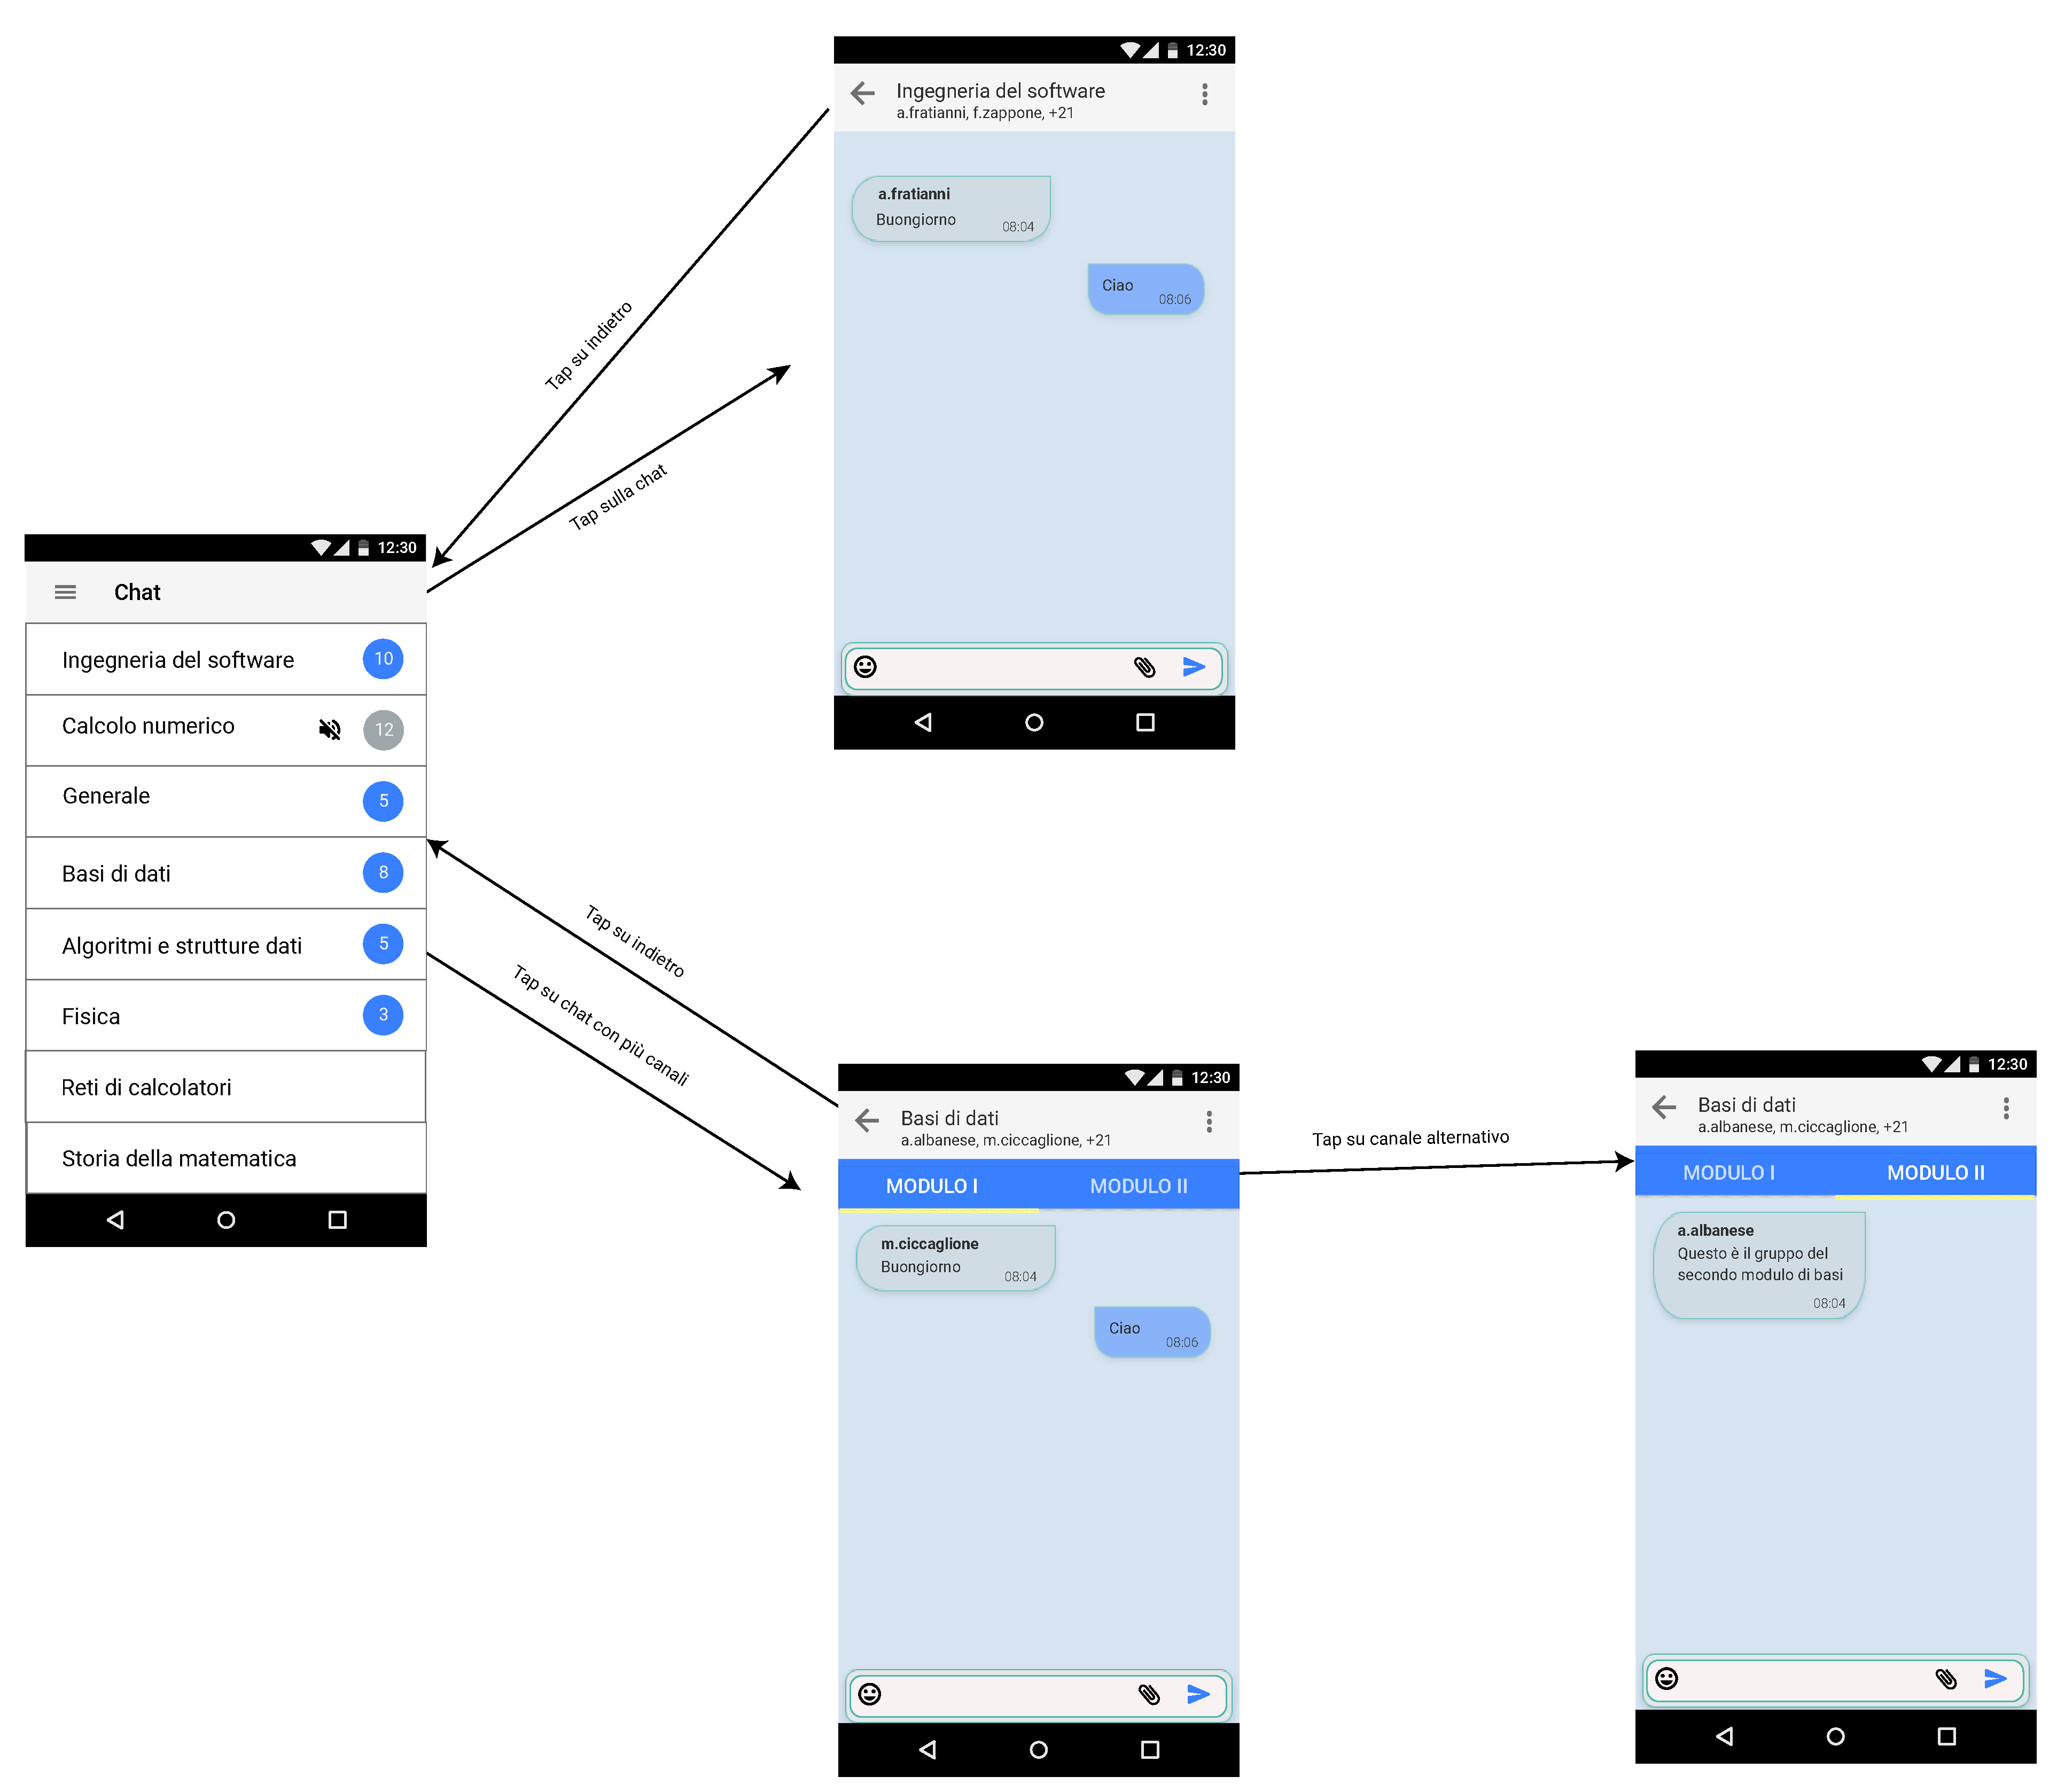
\includegraphics[width=0.9\textwidth]{imgs/gruppo6/activities/act_cus1_visualizza_canale.pdf}
	\caption{CUS 1 - Visualizza canale}
	\label{fig:cus1}
\end{figure}

\begin{figure}
	\centering
	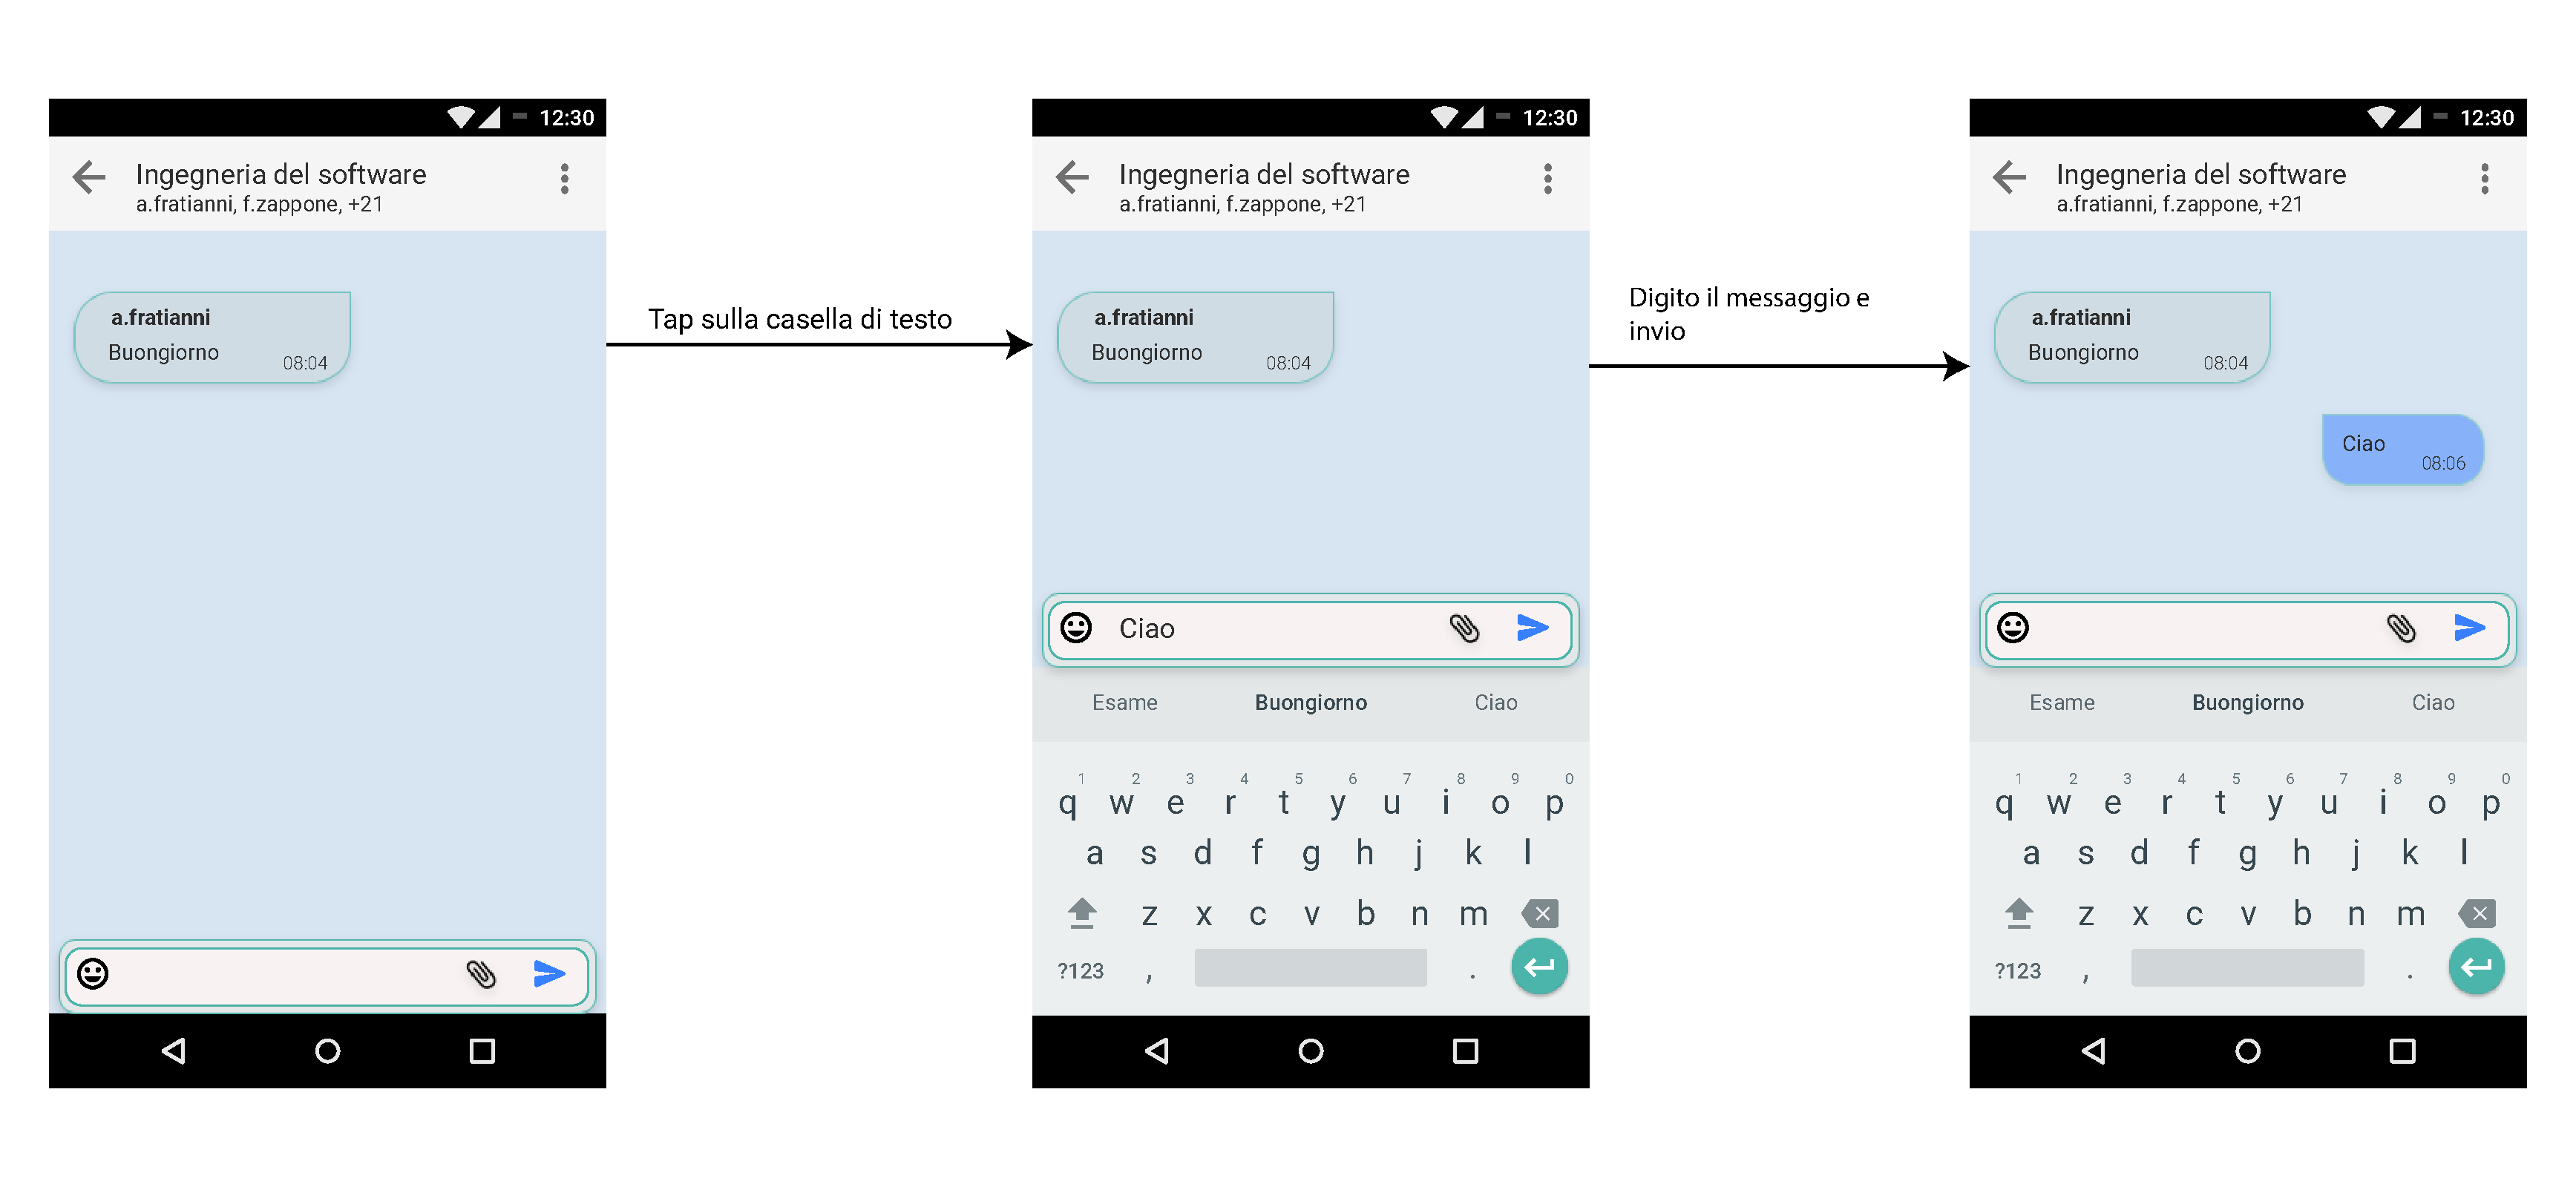
\includegraphics[width=0.9\textwidth]{imgs/gruppo6/activities/act_cus2_invio_messaggio.pdf}
	\caption{CUS2 - Invio messaggio}
	\label{fig:cus2}
\end{figure}

\begin{figure}
	\centering
	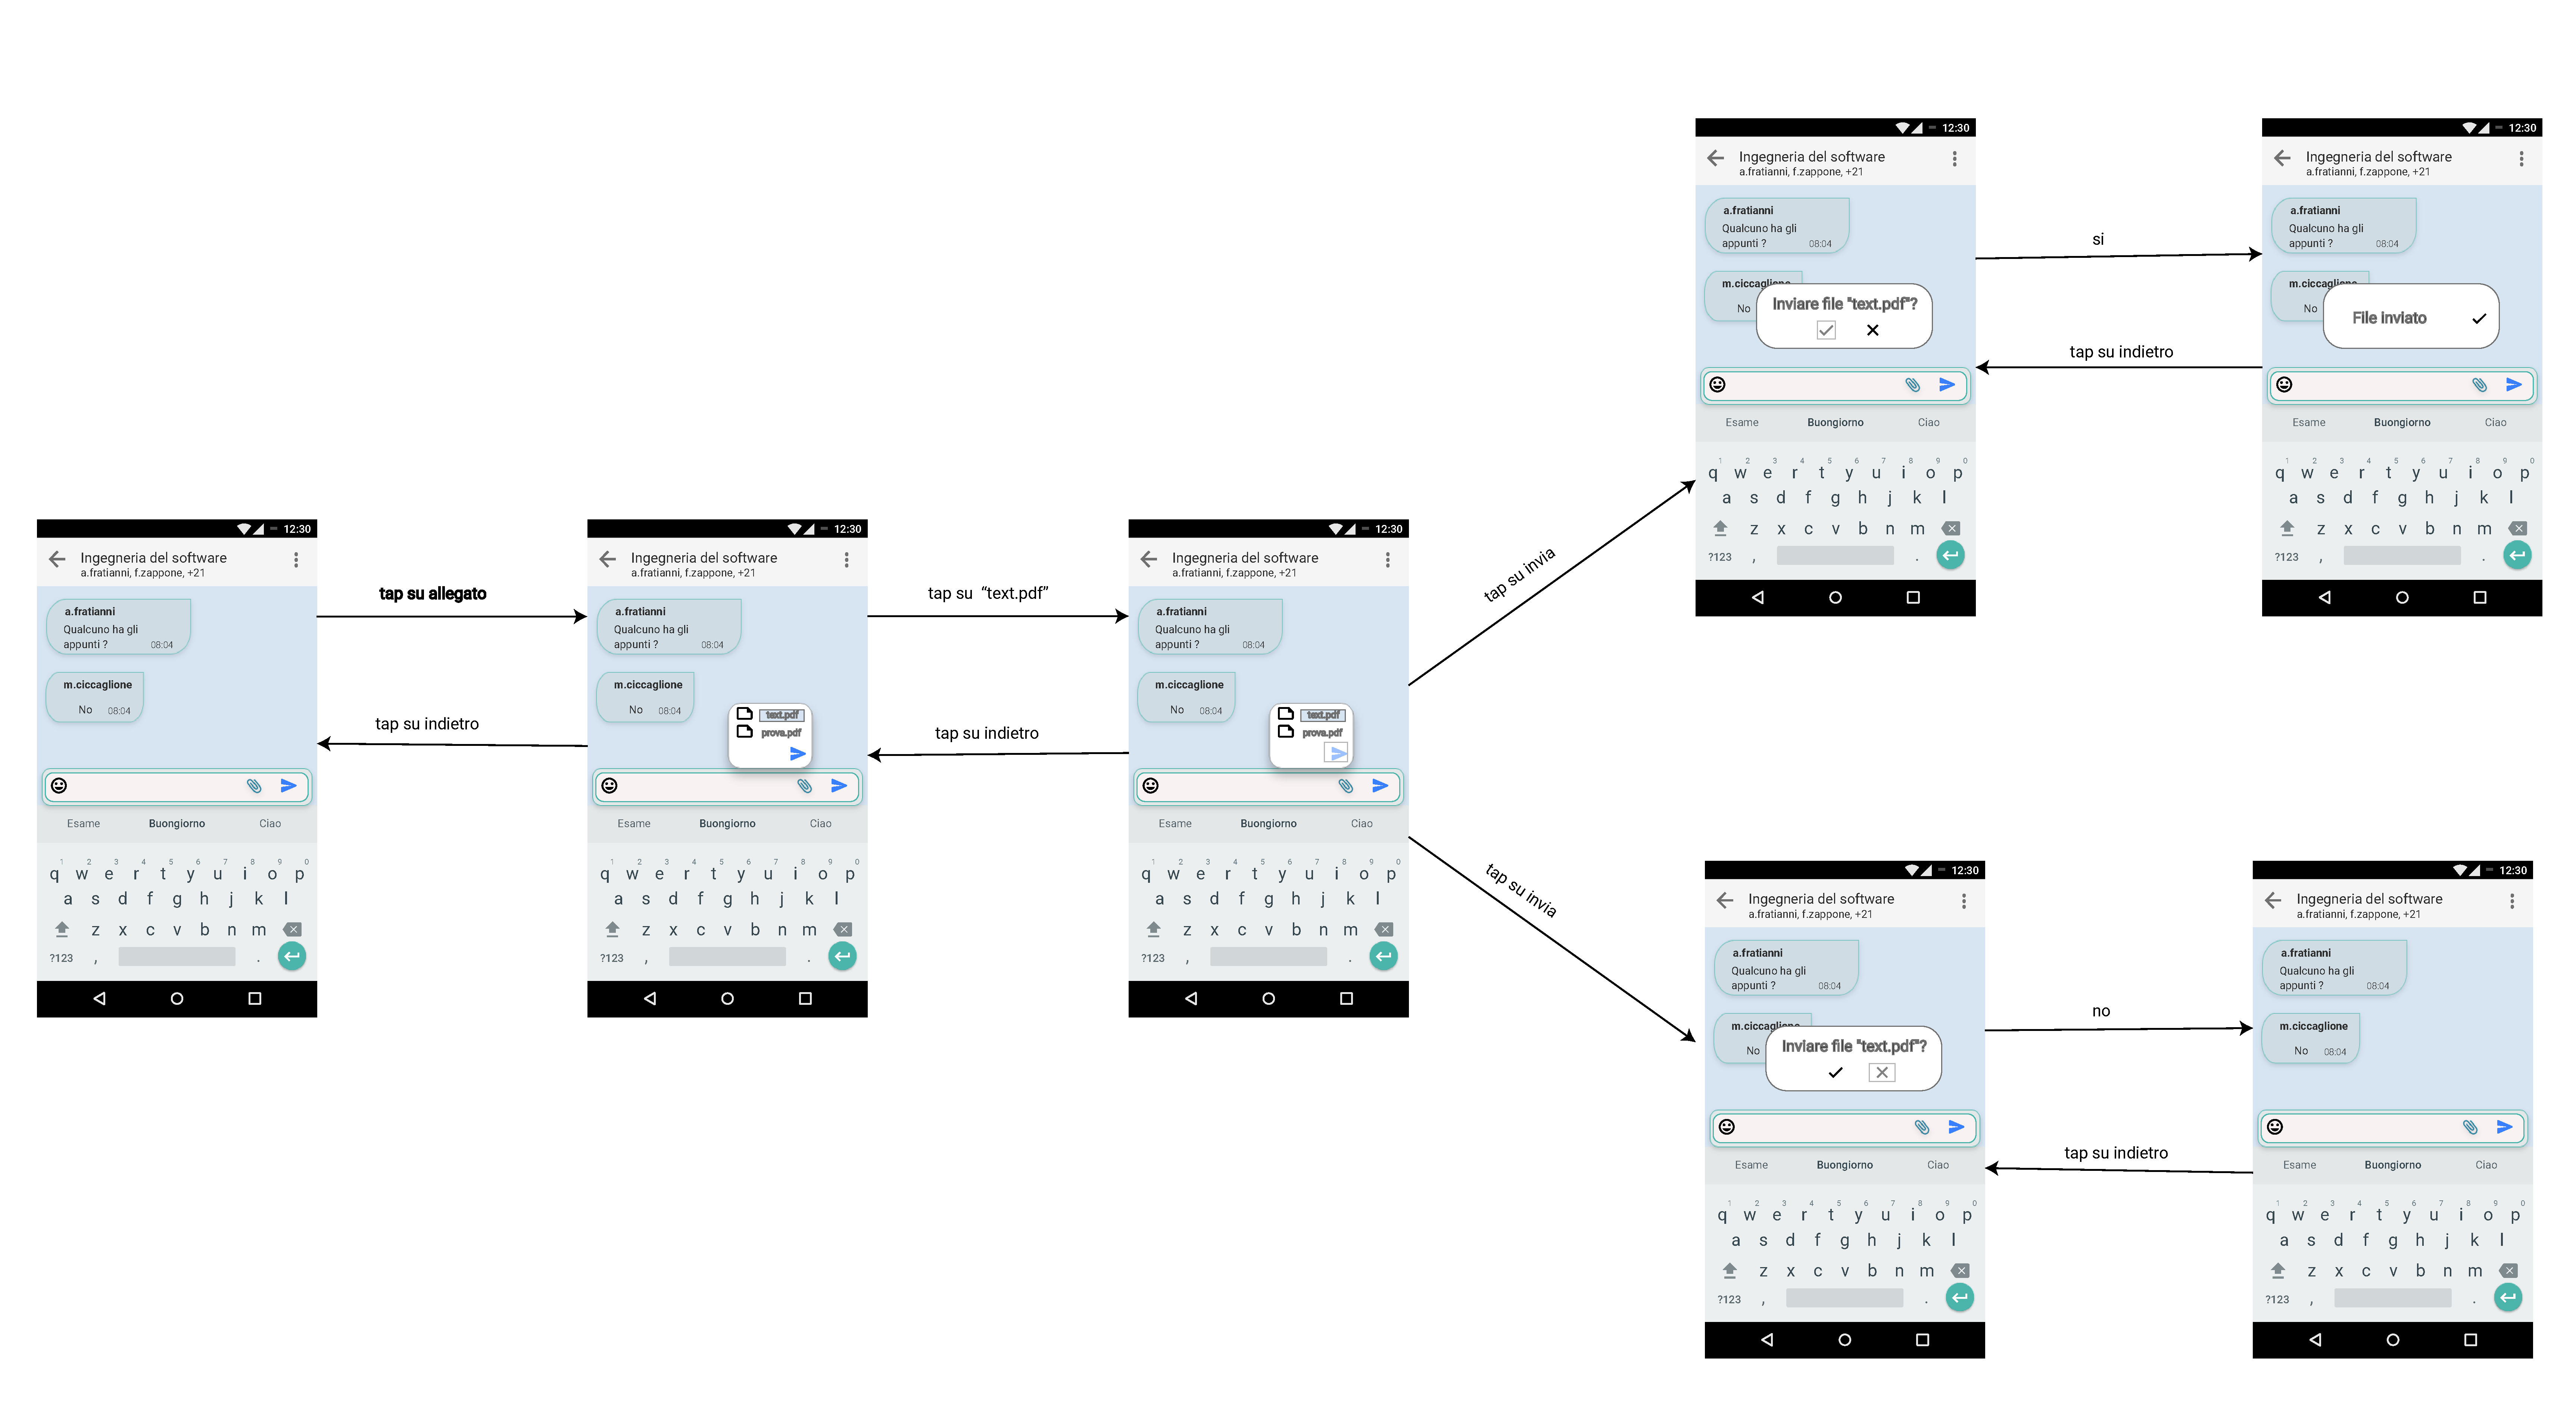
\includegraphics[width=0.9\textwidth]{imgs/gruppo6/activities/act_cus3_invia_allegato.pdf}
	\caption{CUS3 - Invio Allegato}
	\label{fig:cus3-1}
\end{figure}

\begin{figure}
	\centering
	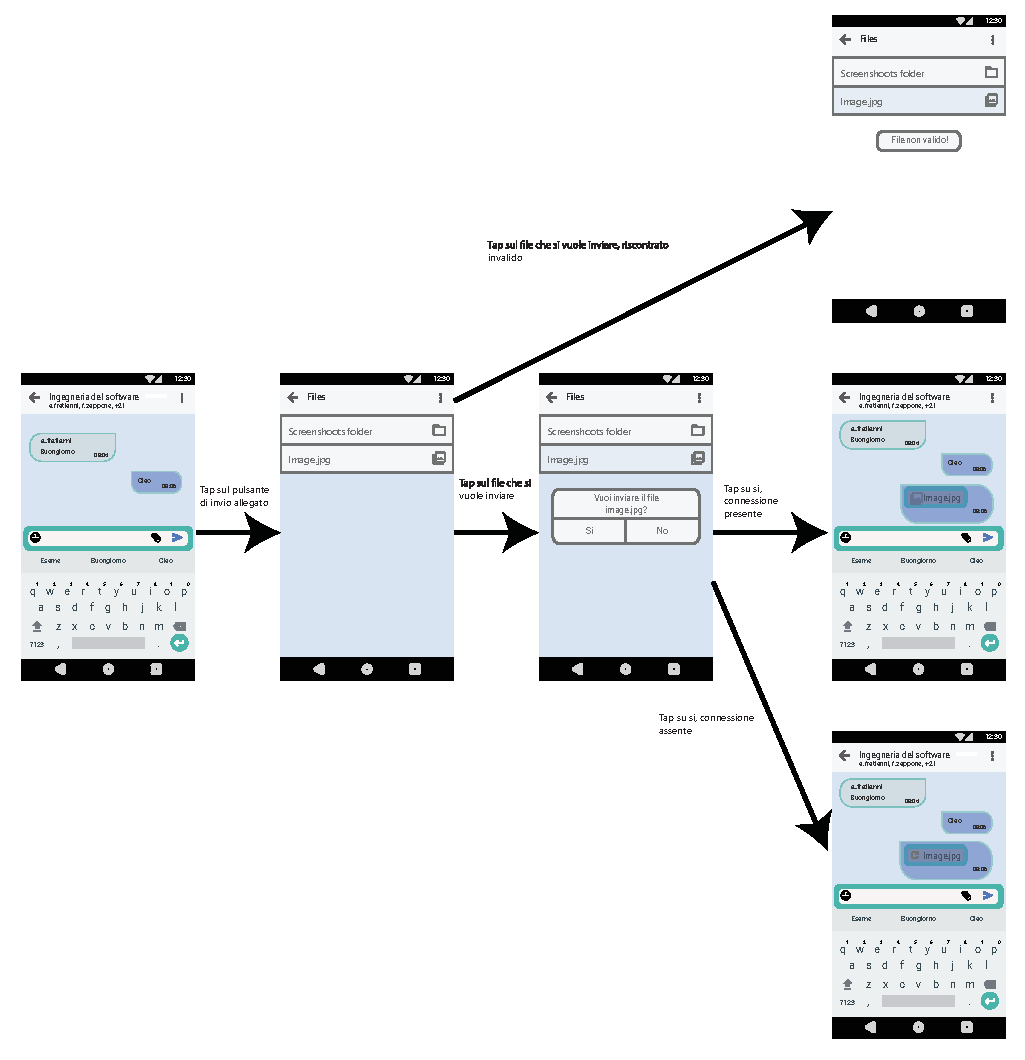
\includegraphics[width=0.9\textwidth]{imgs/gruppo6/activities/act_cus3_invio_allegato2.pdf}
	\caption{CUS3 - Invio Allegato (es. 2)}
	\label{fig:cus3-2}
\end{figure}

\begin{figure}
	\centering
	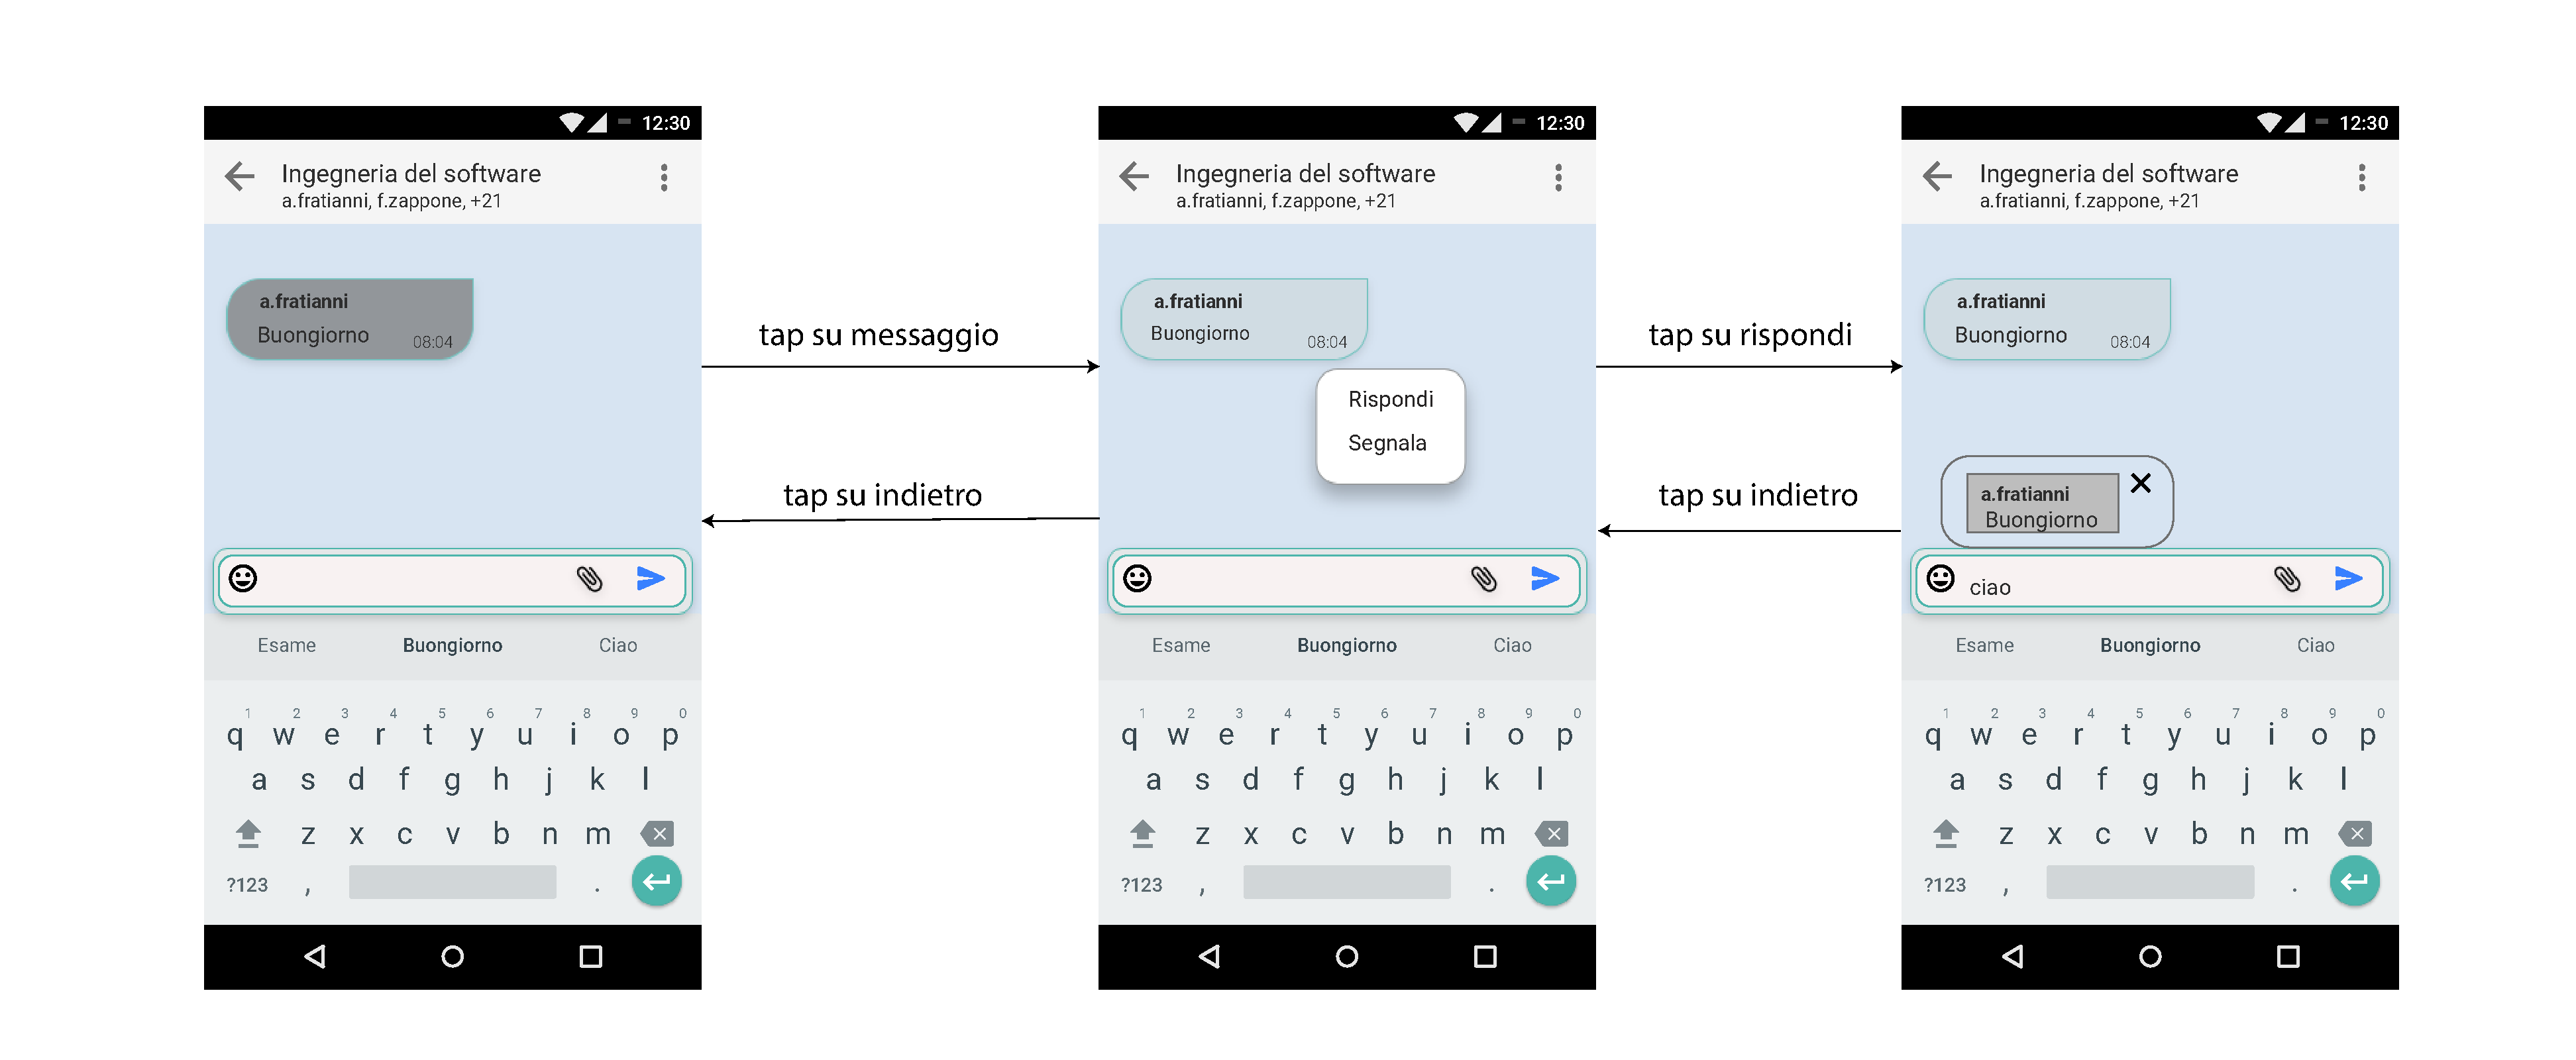
\includegraphics[width=0.9\textwidth]{imgs/gruppo6/activities/act_cus4_rispondi_singolo_messaggio.pdf}
	\caption{CUS4 - Rispondi al messaggio}
	\label{fig:cus4}
\end{figure}

\begin{figure}
	\centering
	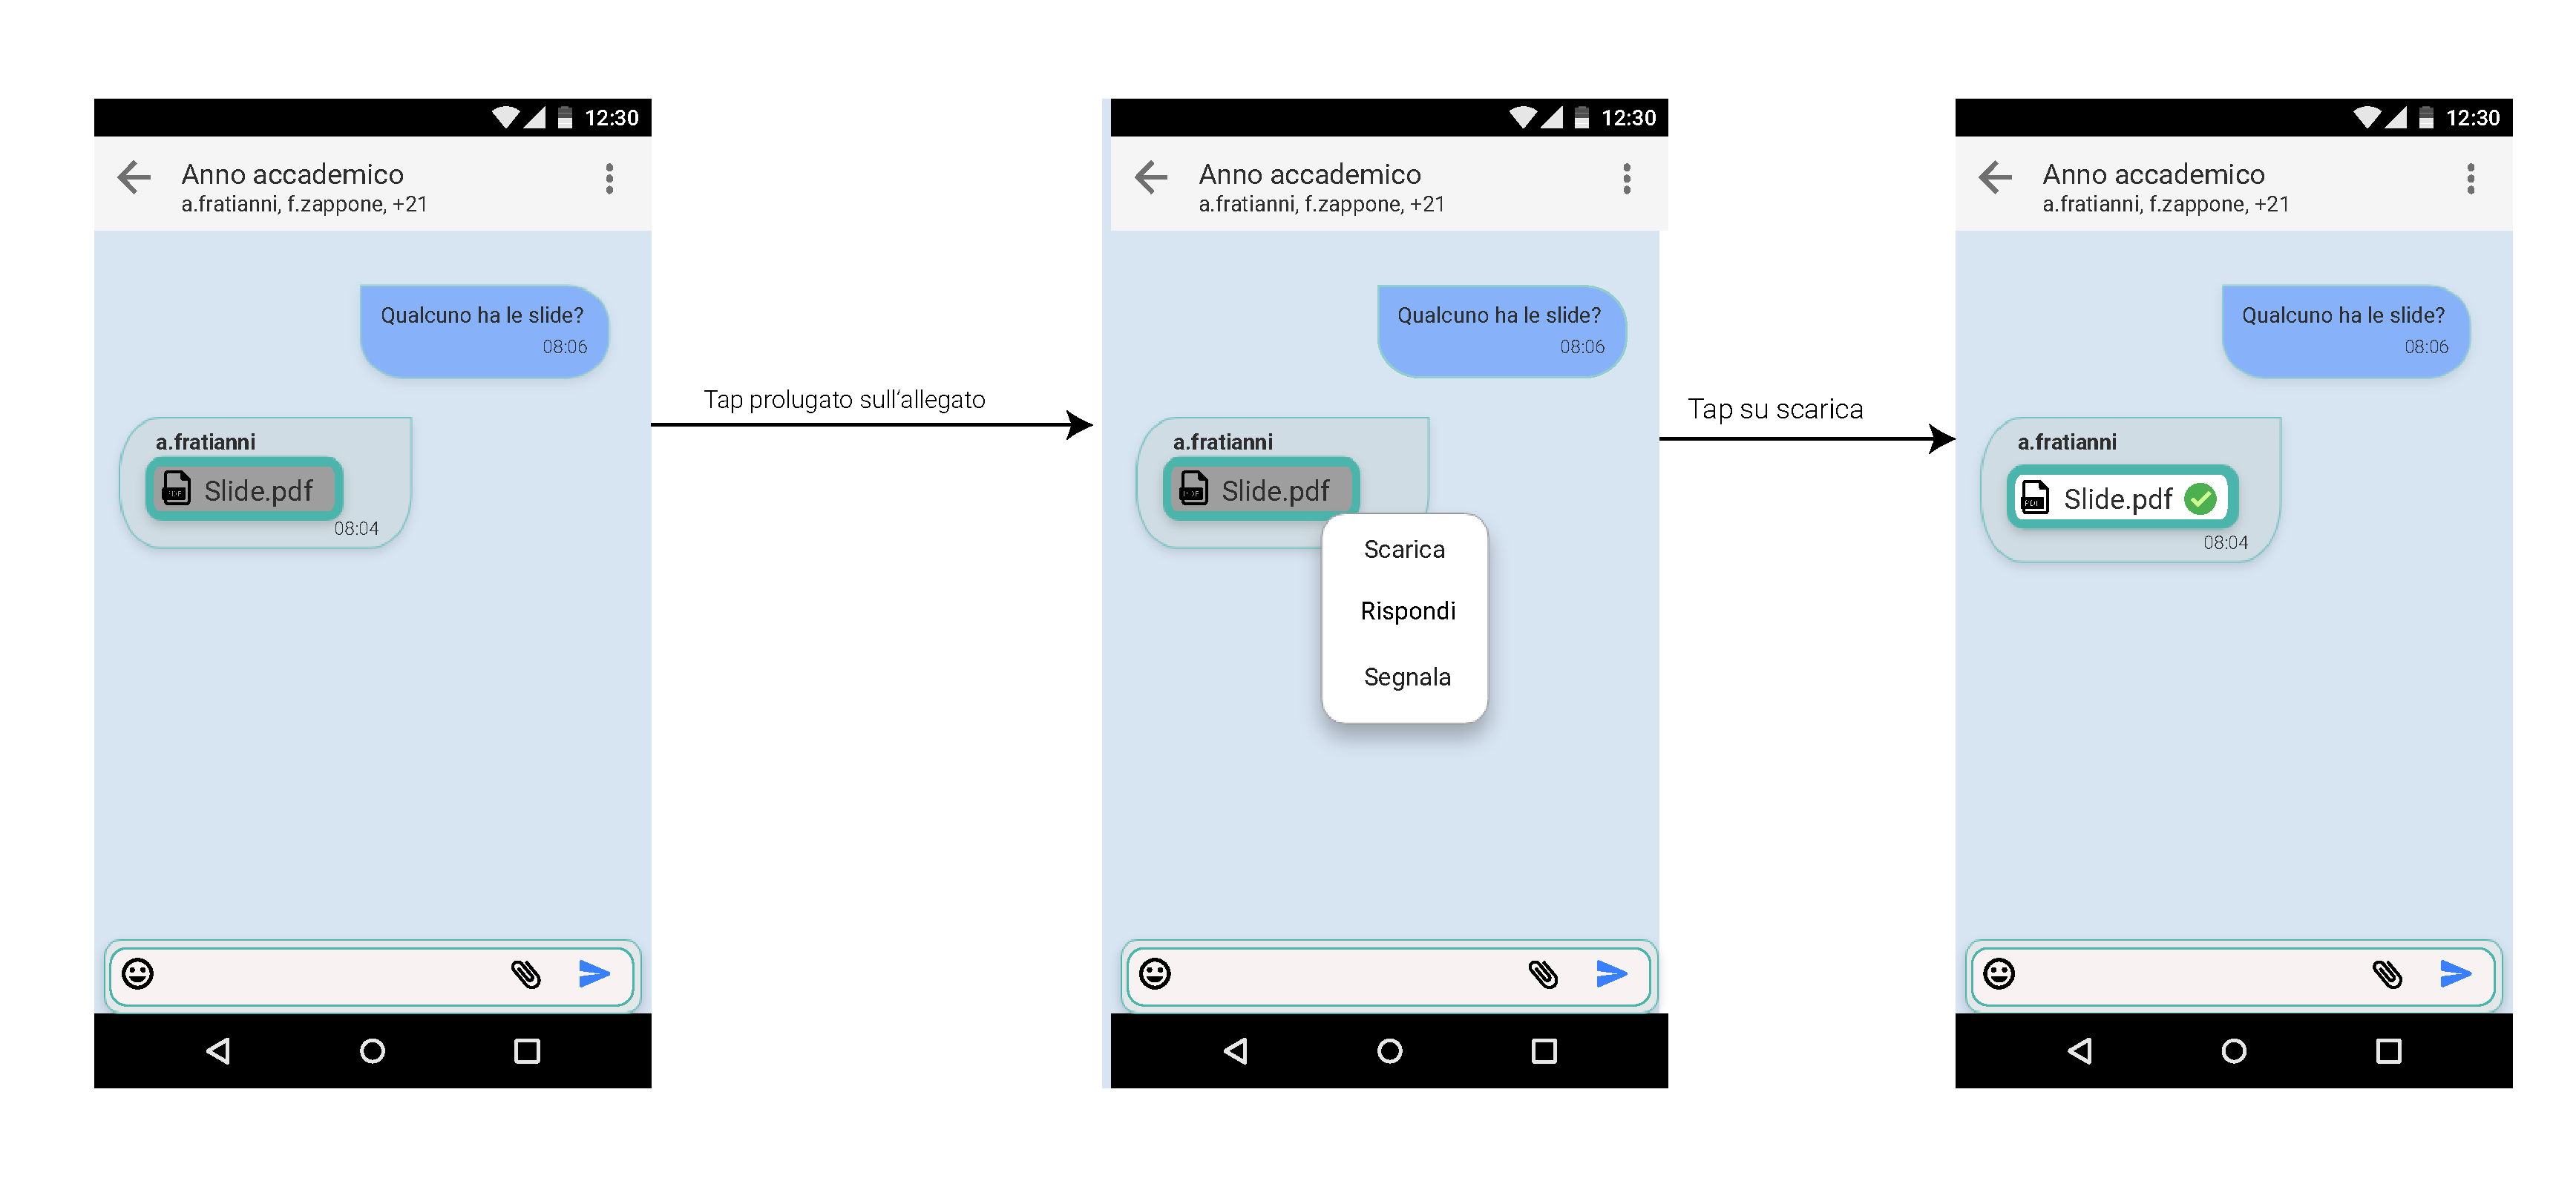
\includegraphics[width=0.9\textwidth]{imgs/gruppo6/activities/act_cus5_scarica_allegato.pdf}
	\caption{CUS5 - Scarica allegato}
	\label{fig:cus5}
\end{figure}

\begin{figure}
	\centering
	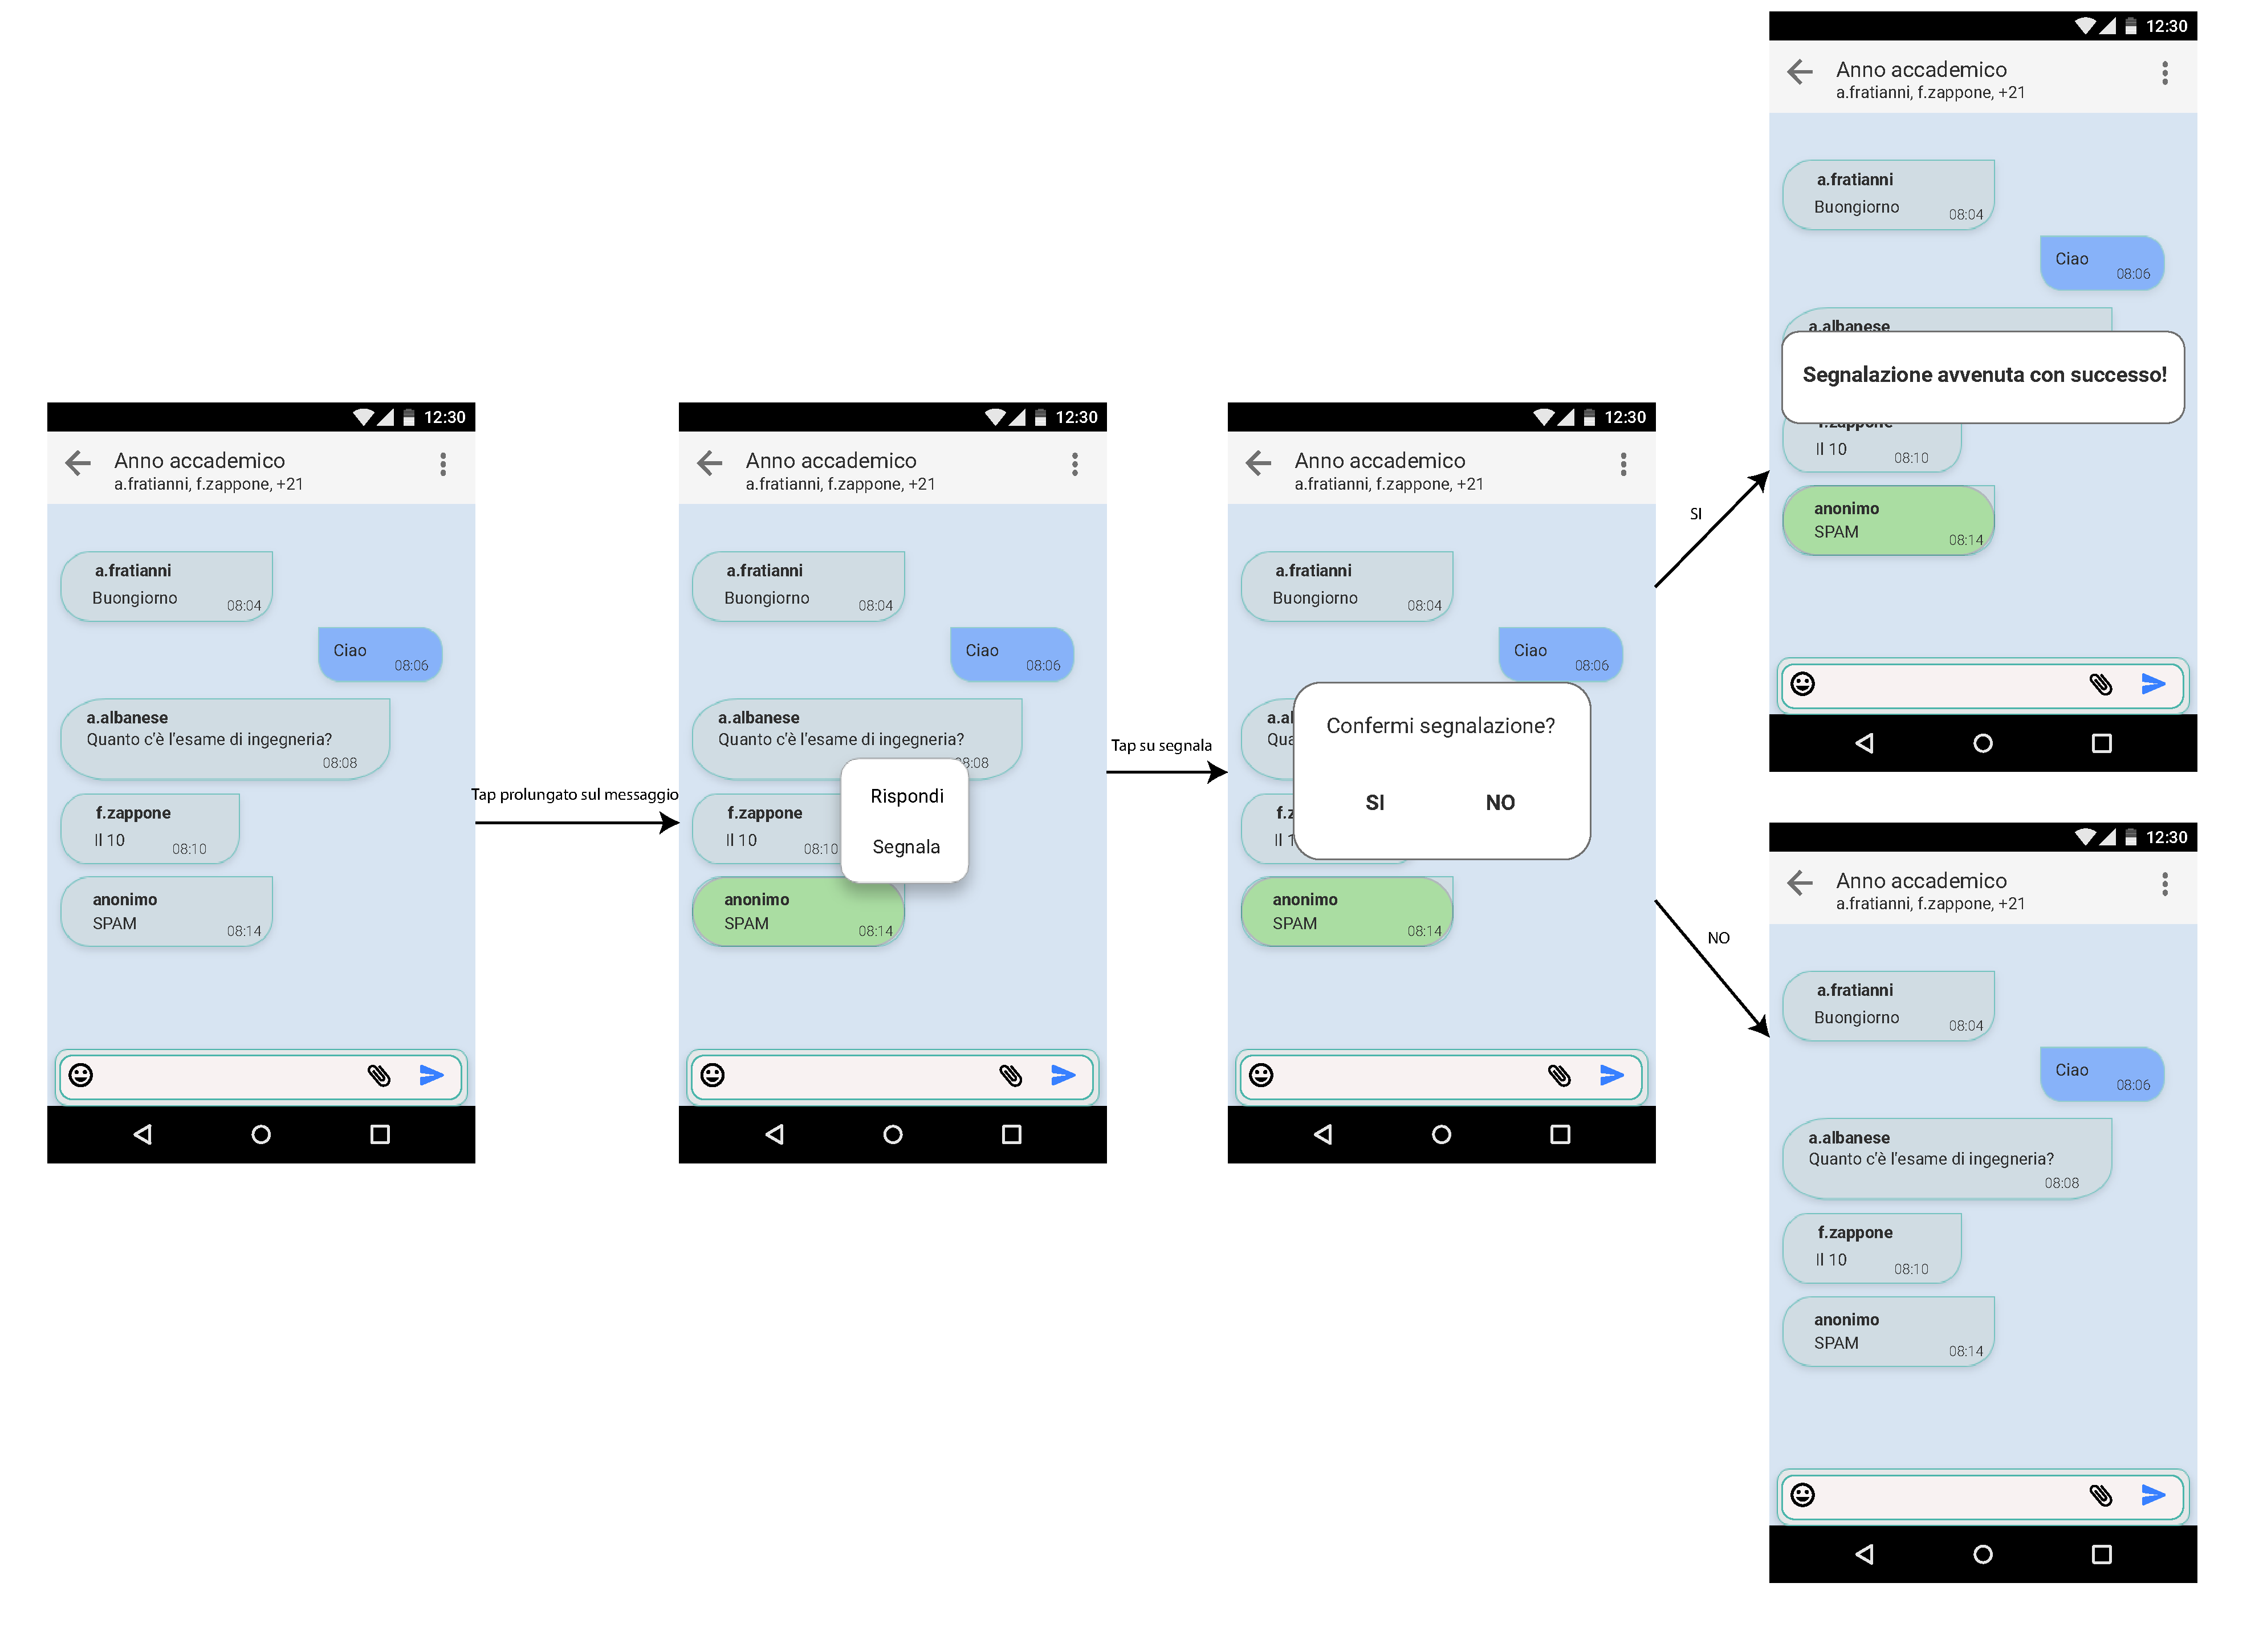
\includegraphics[width=0.9\textwidth]{imgs/gruppo6/activities/act_cus6_segnalazione_messaggio.pdf}
	\caption{CUS6 - Segnalazione messaggio}
	\label{fig:cus6}
\end{figure}

\begin{figure}
	\centering
	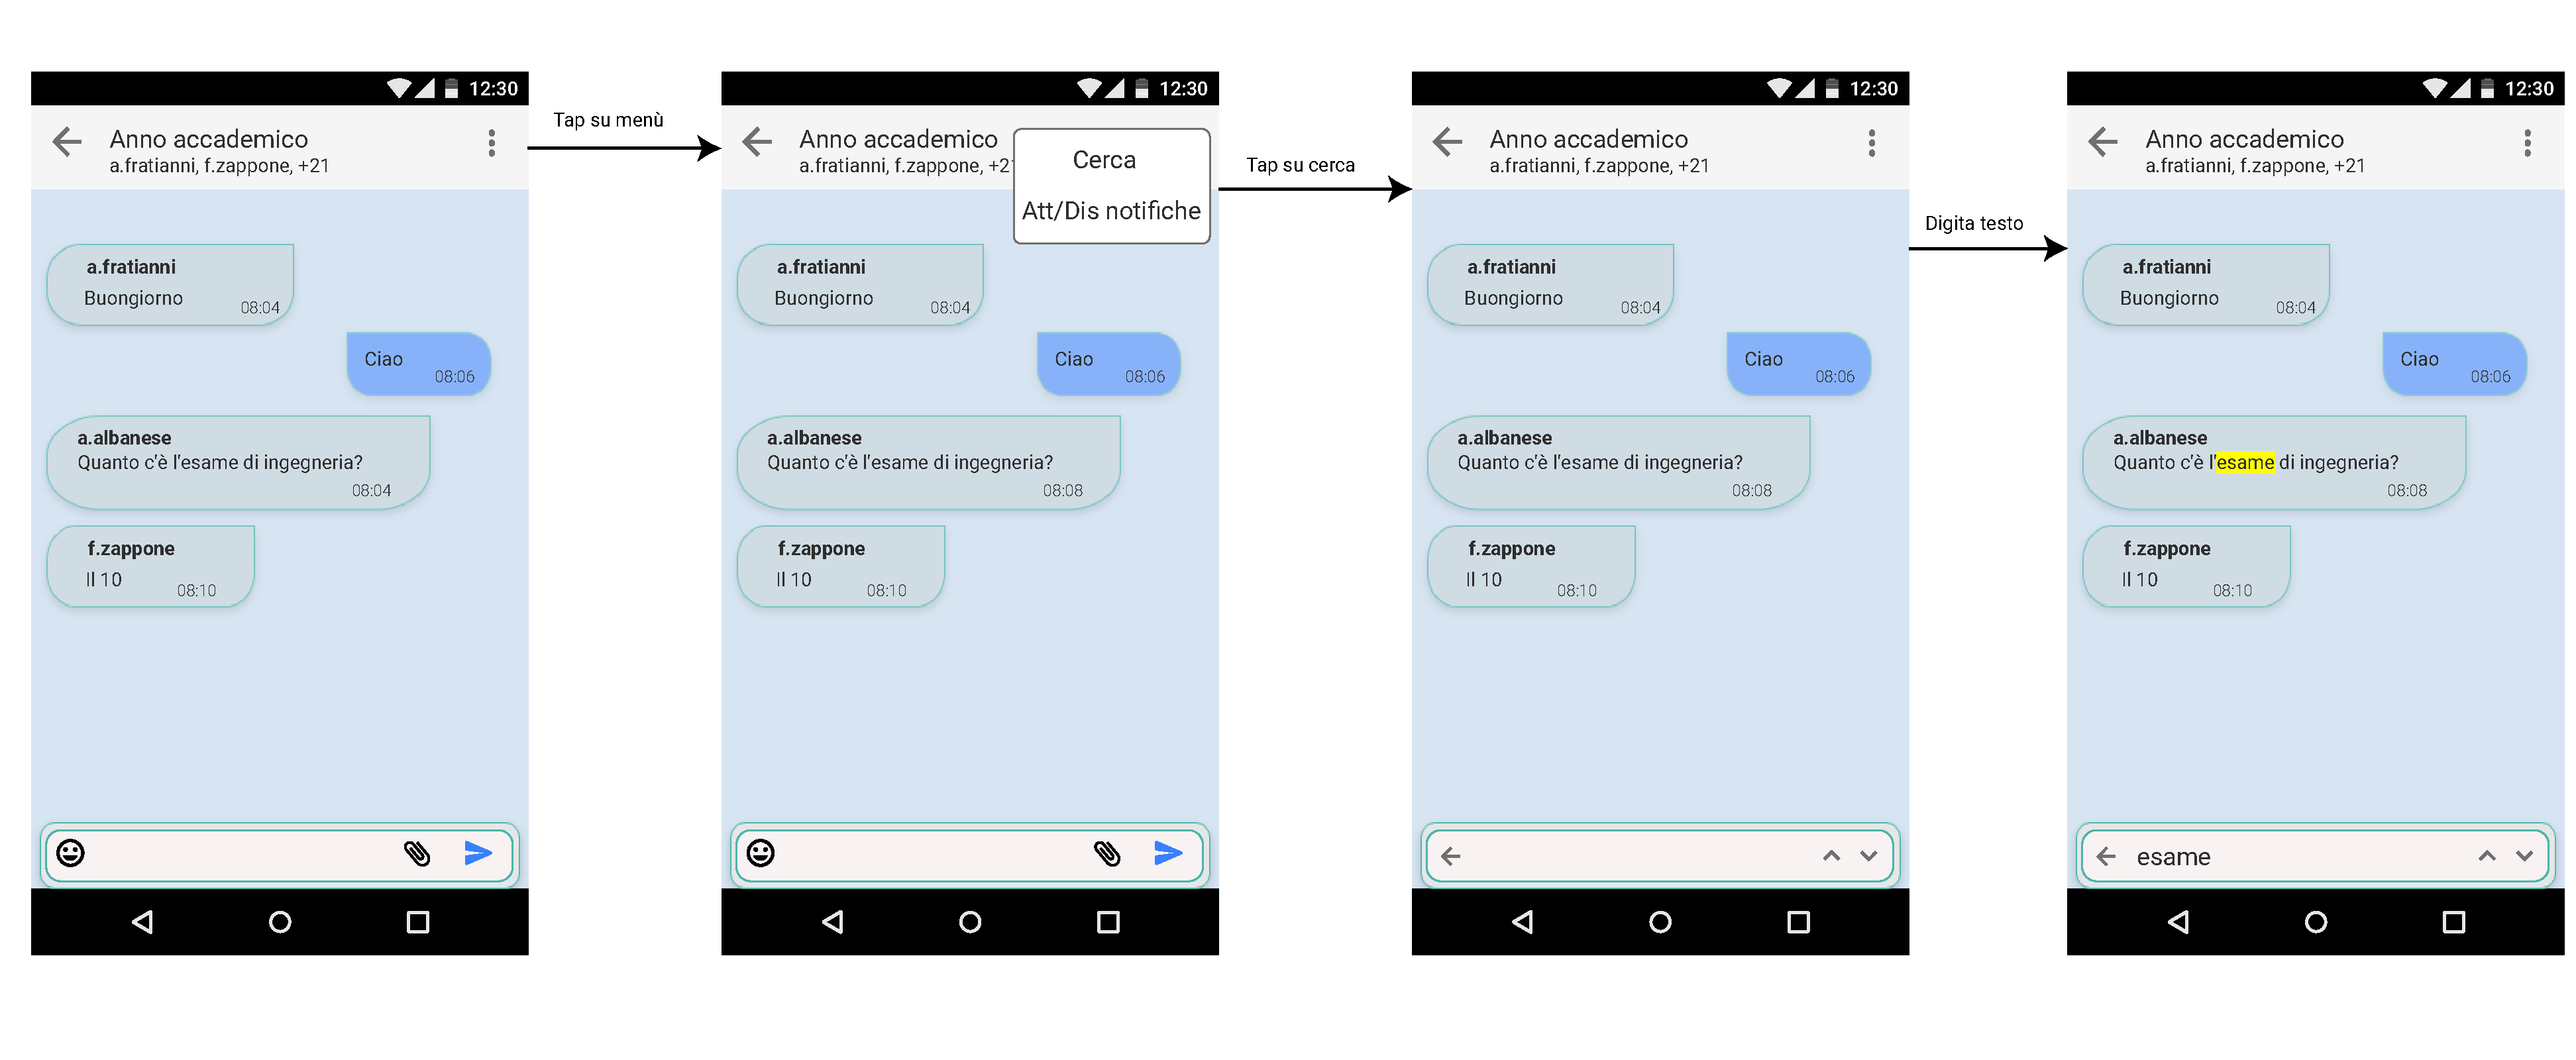
\includegraphics[width=0.9\textwidth]{imgs/gruppo6/activities/act_cus7_ricerca_testo_nella_chat.pdf}
	\caption{CUS7 - Ricerca testo nella chat}
	\label{fig:cus7}
\end{figure}

\begin{figure}
	\centering
	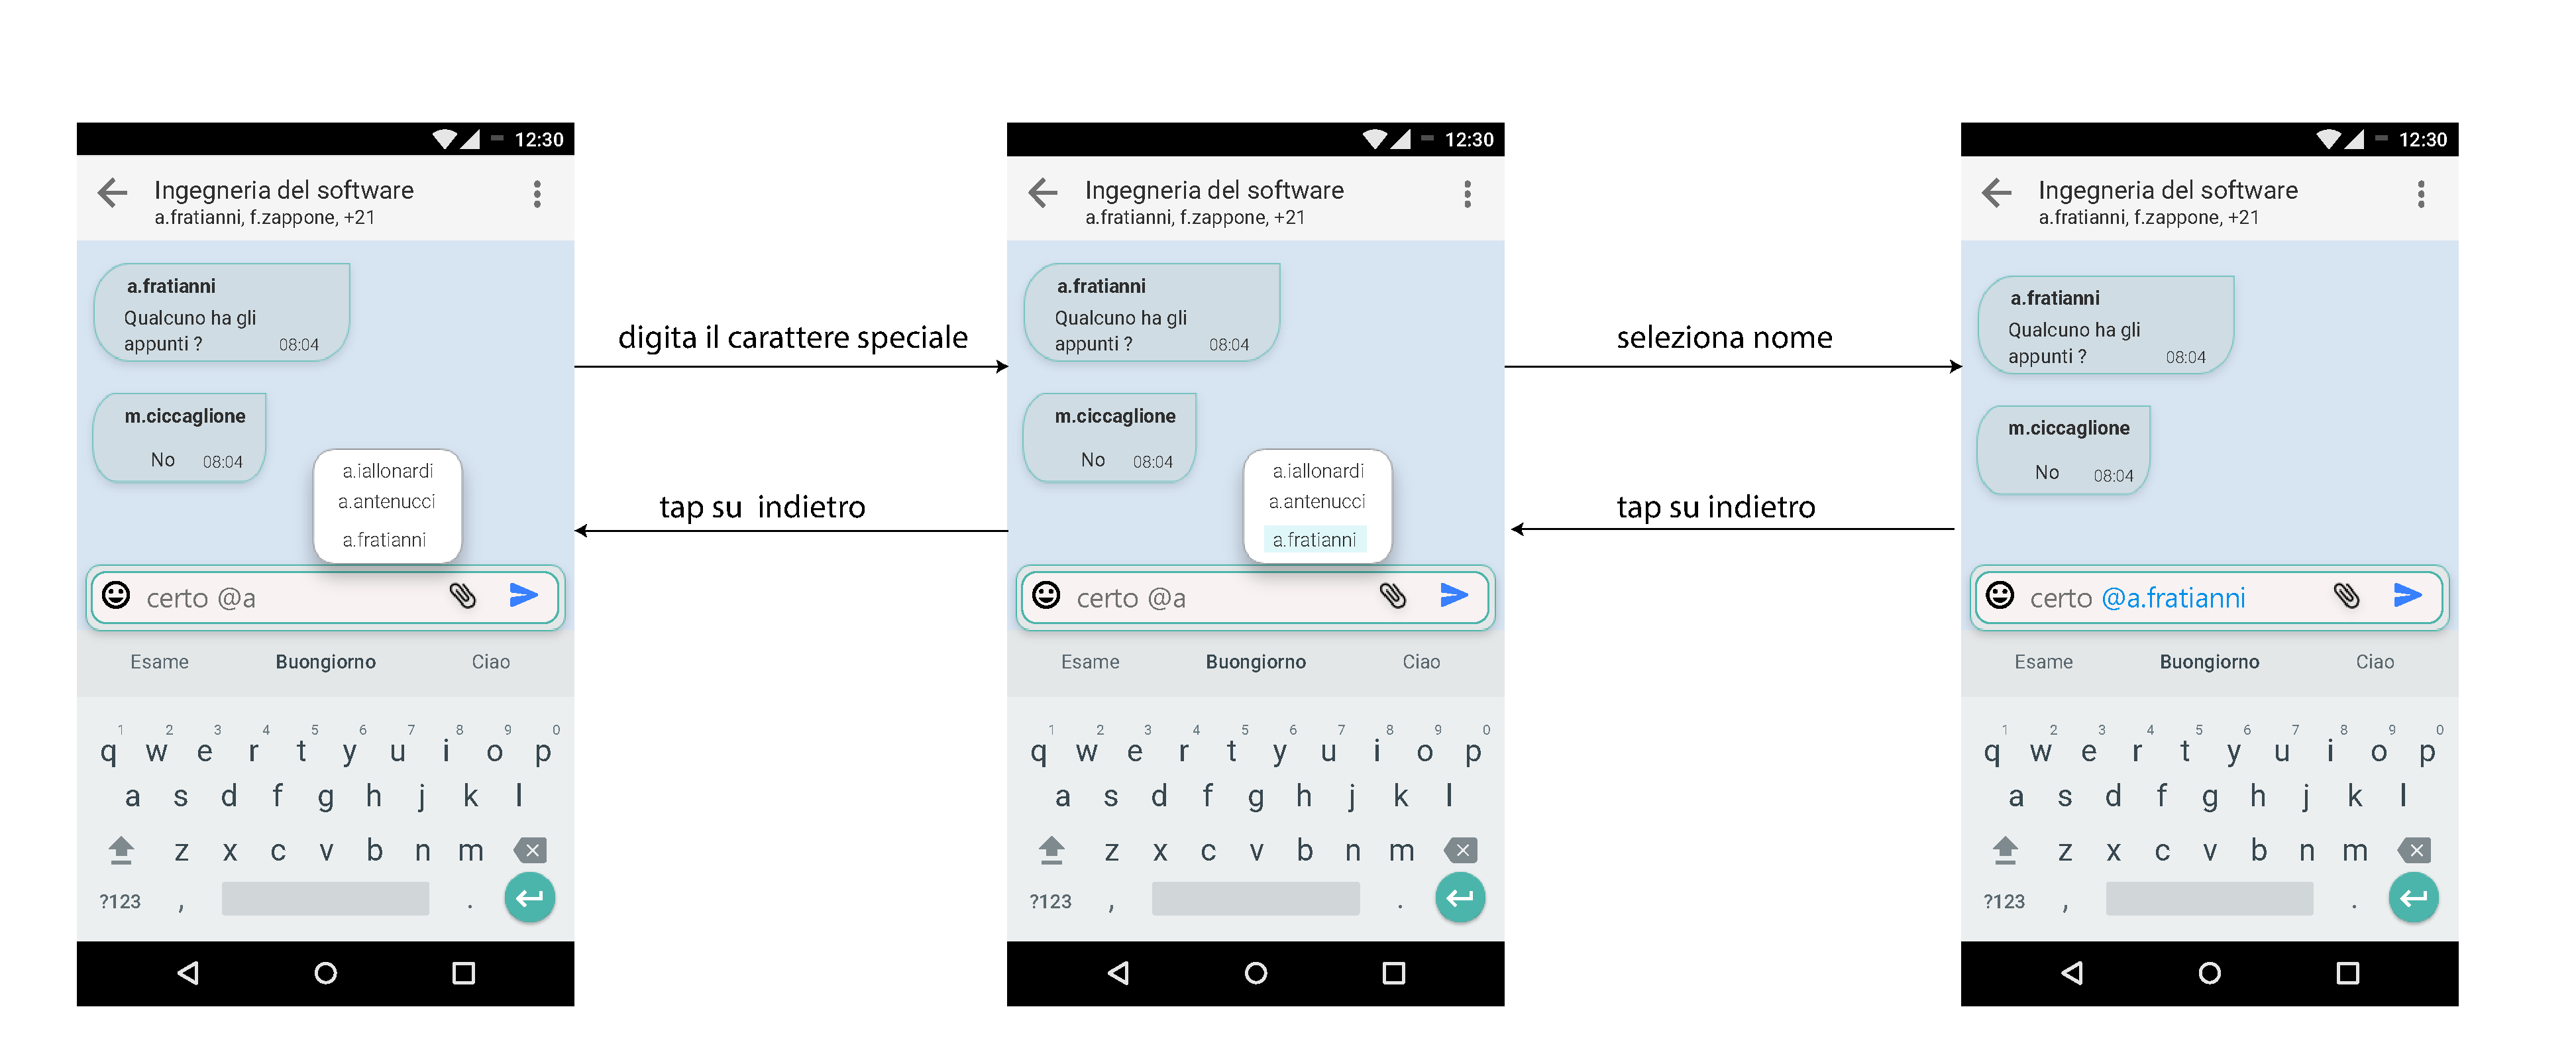
\includegraphics[width=0.9\textwidth]{imgs/gruppo6/activities/act_cus8_tag_membro_messaggio.pdf}
	\caption{CUS8 - Tag membro in messaggio}
	\label{fig:cus8}
\end{figure}

\begin{figure}
	\centering
	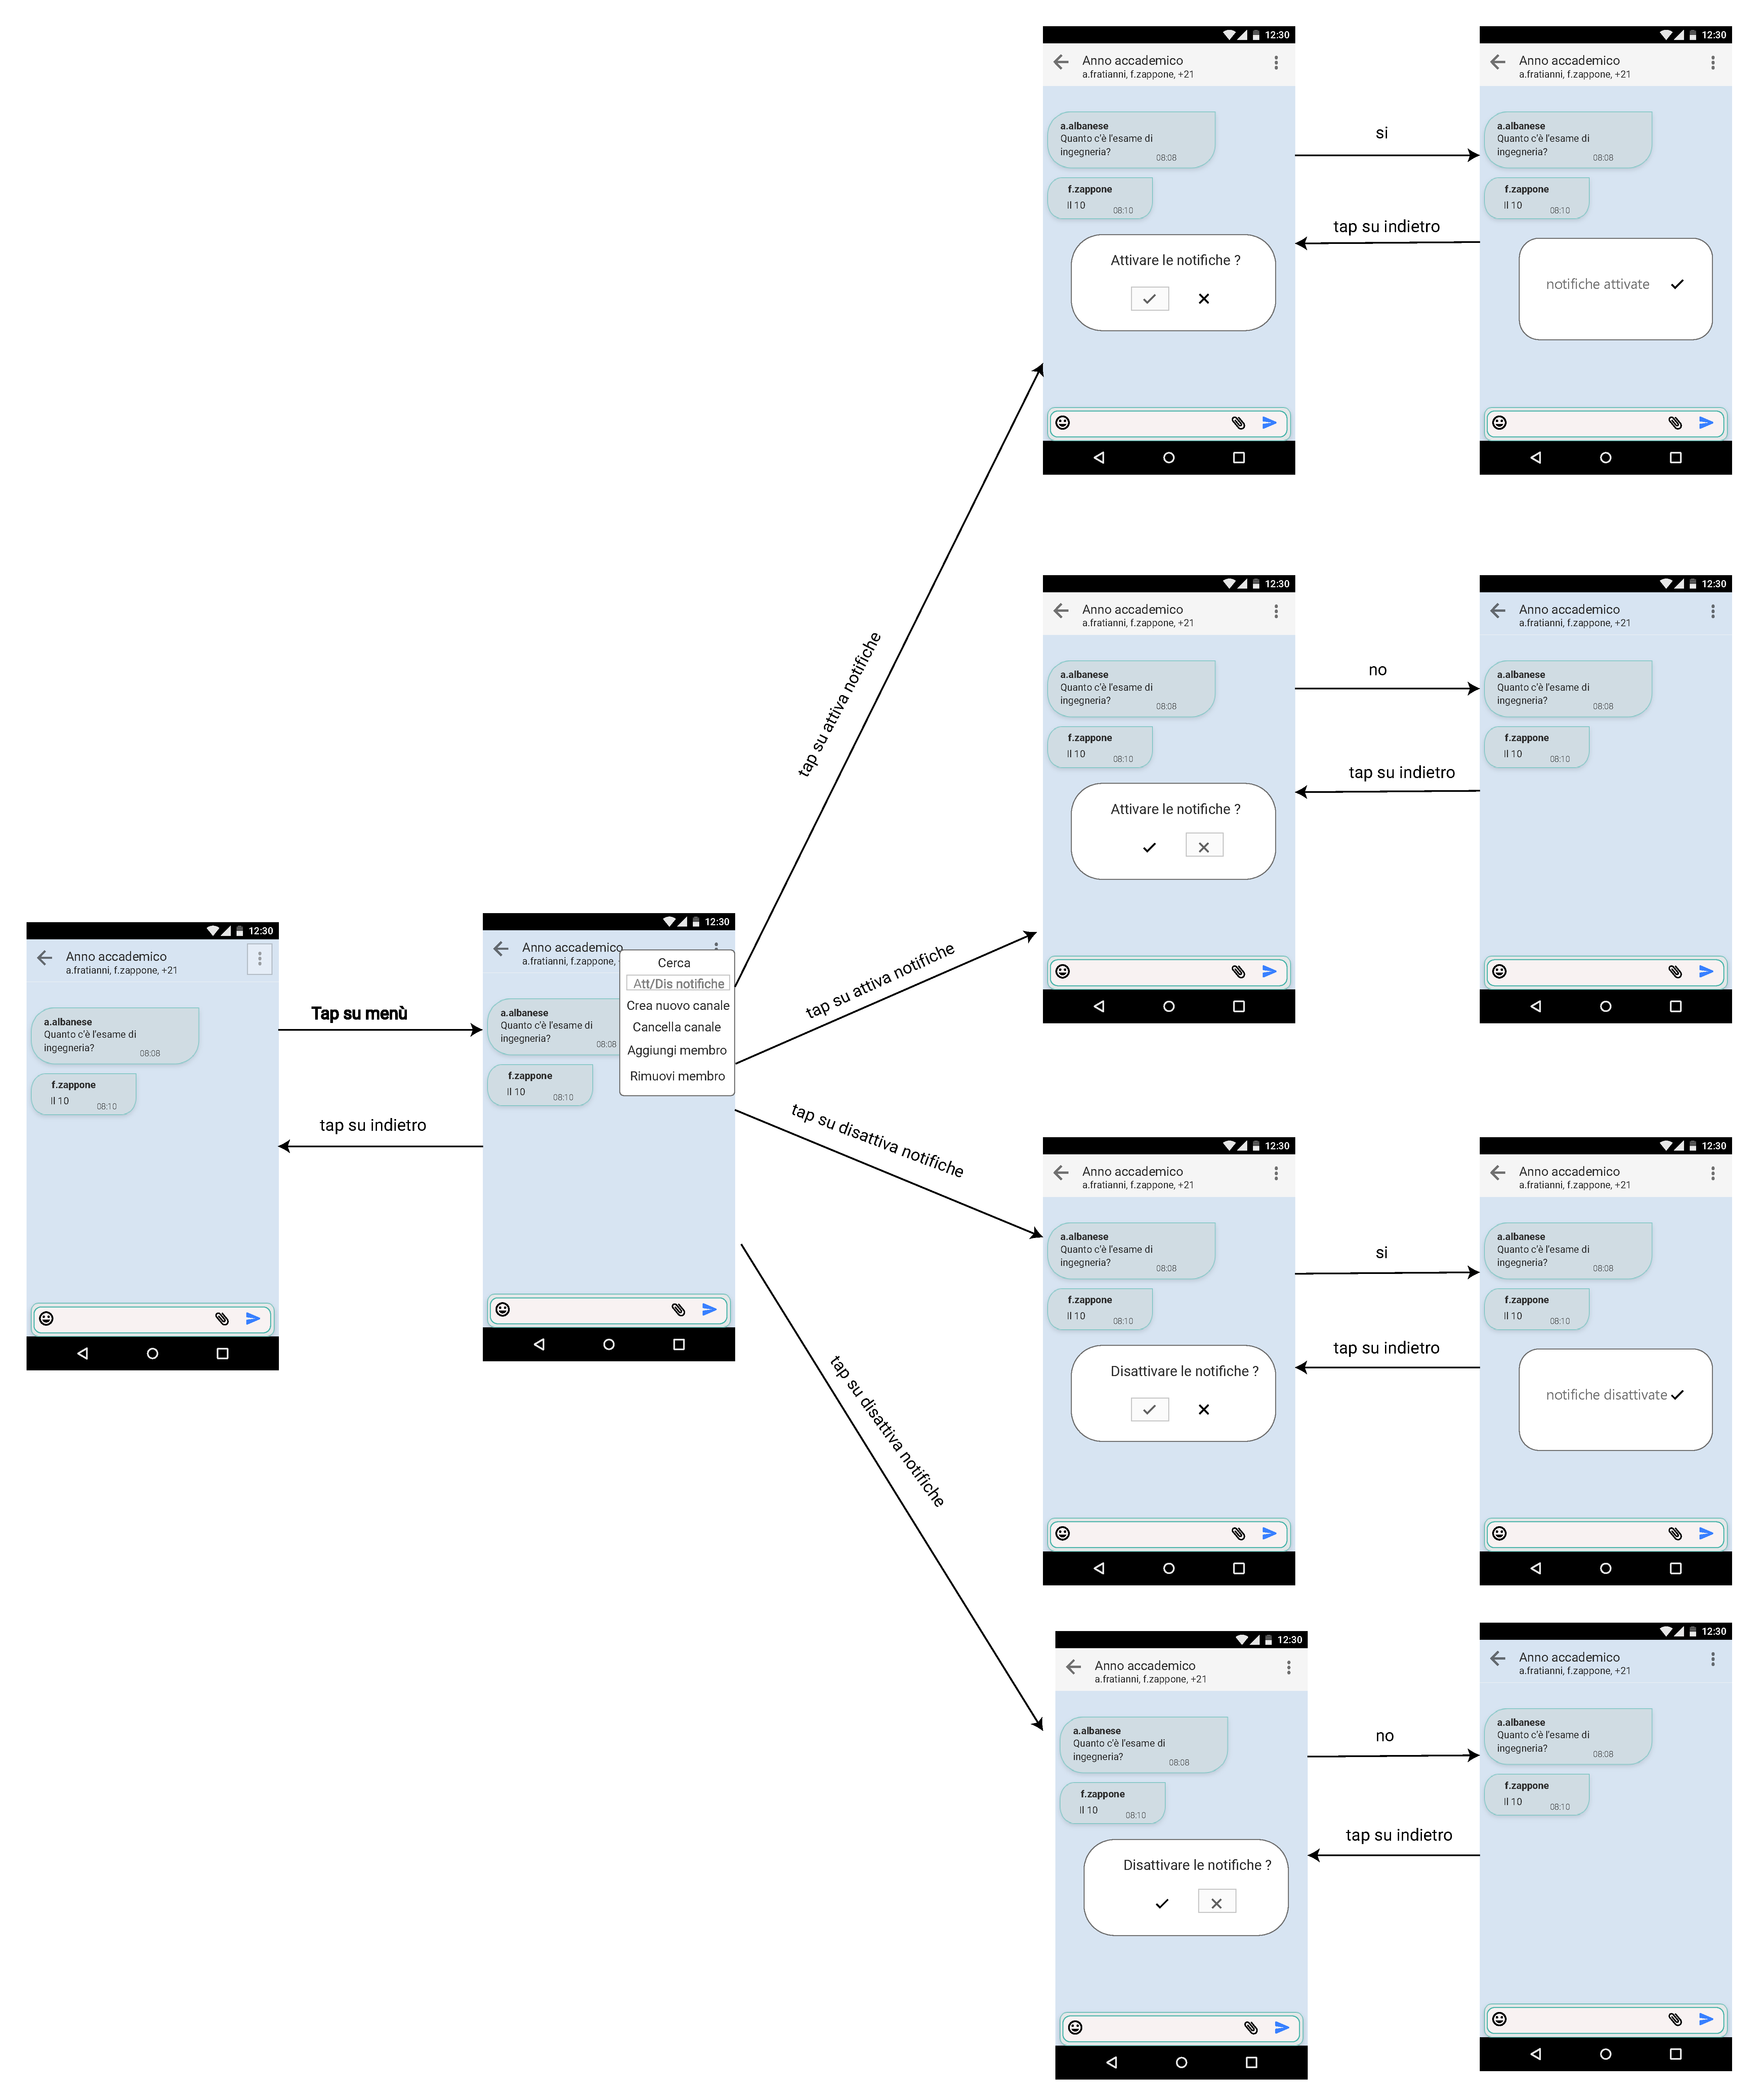
\includegraphics[width=0.9\textwidth]{imgs/gruppo6/activities/act_cus9_gestisci_notifiche_chat.pdf}
	\caption{CUS9 - Gestisci notifiche chat}
	\label{fig:cus9}
\end{figure}

\begin{figure}
	\centering
	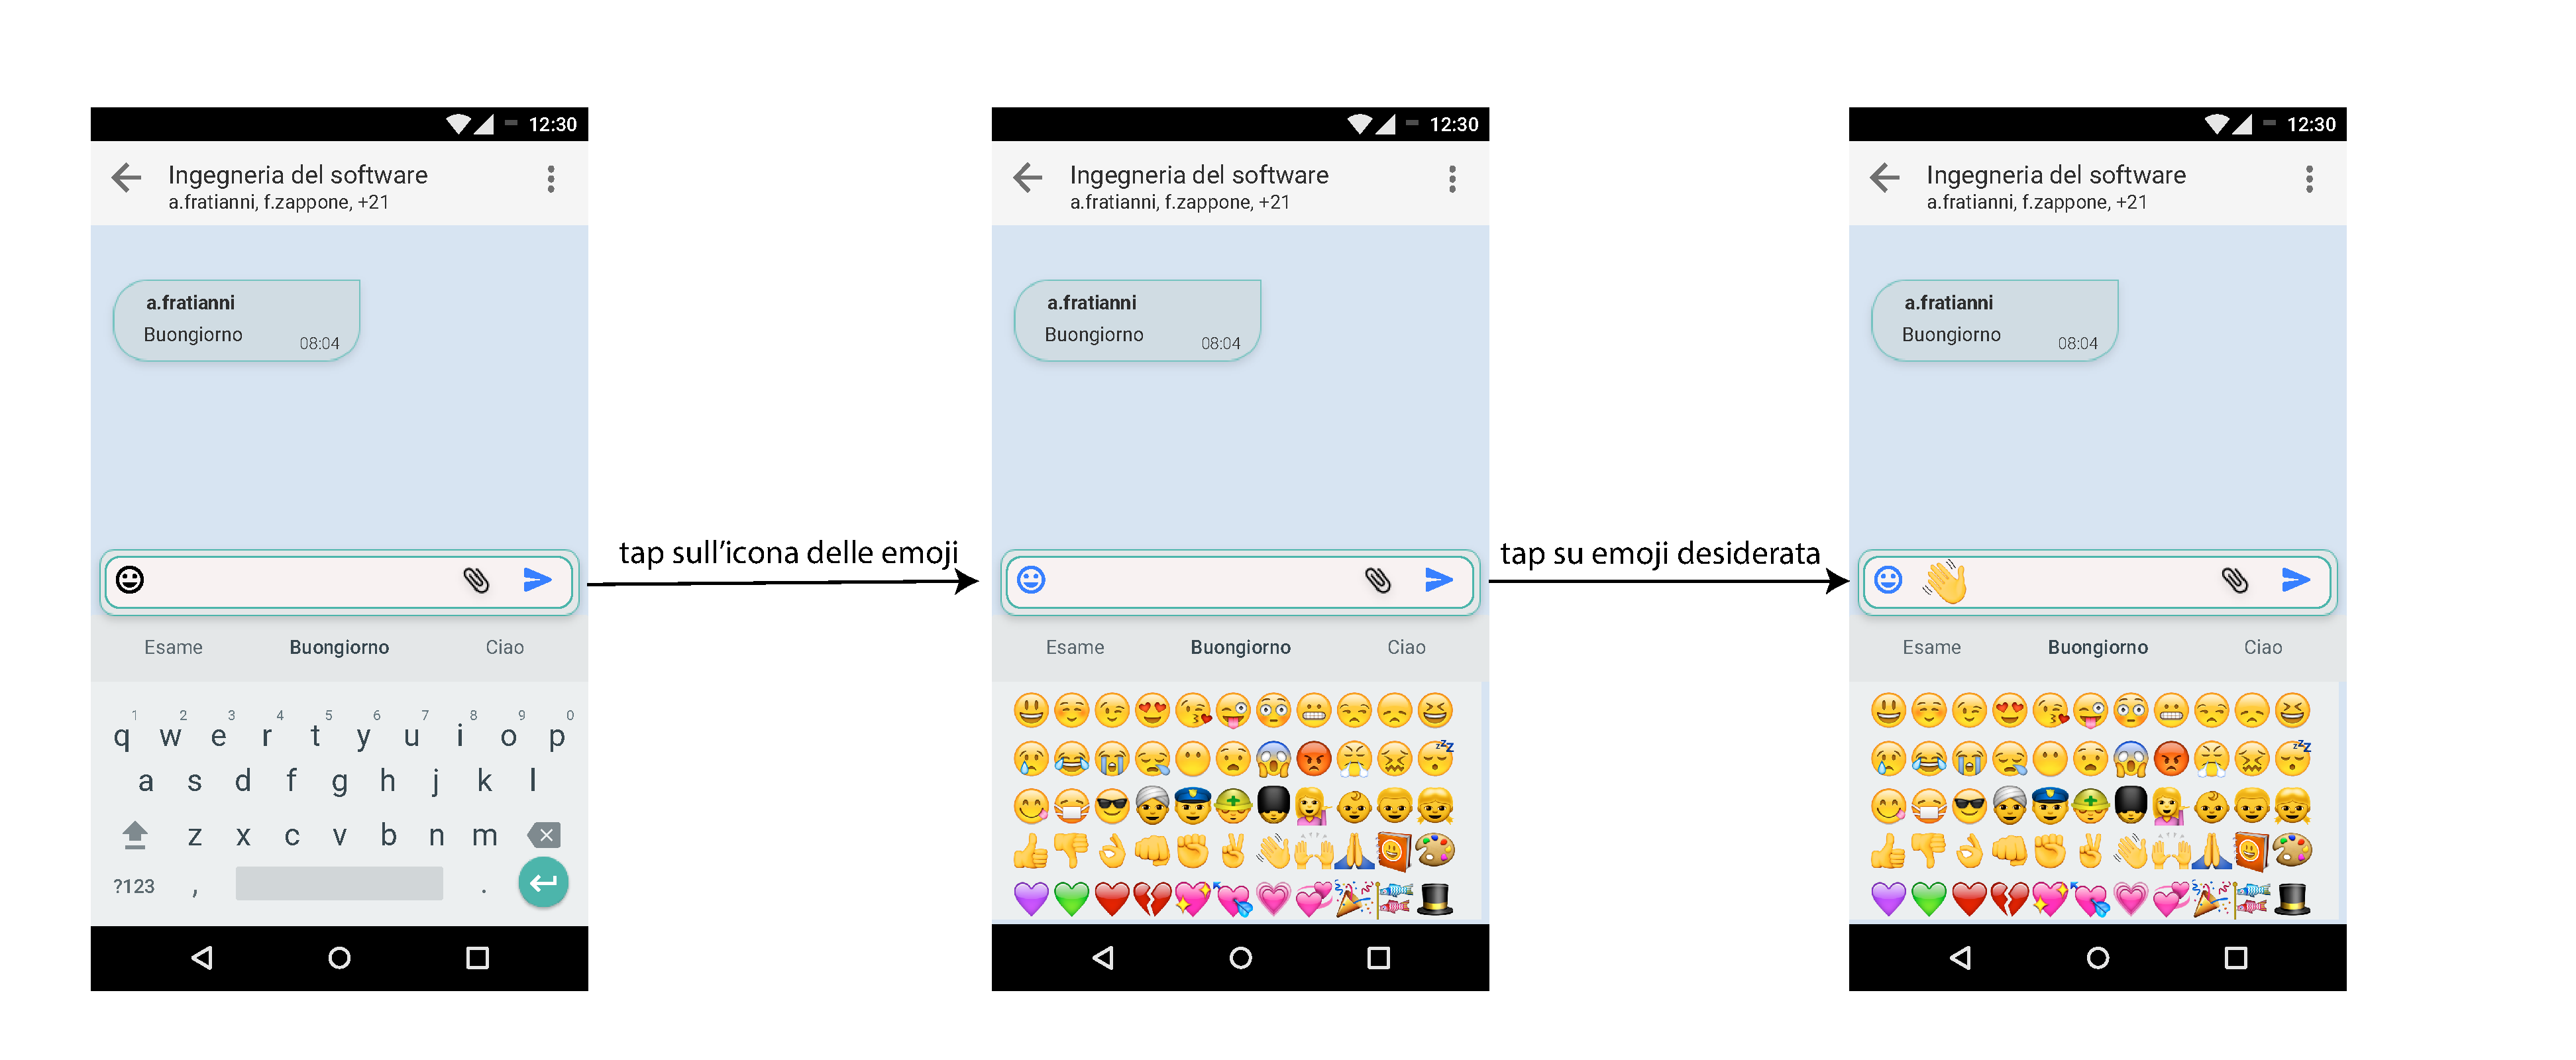
\includegraphics[width=0.9\textwidth]{imgs/gruppo6/activities/act_cus10_seleziona_emoji.pdf}
	\caption{CUS10 - Selezione emoji}
	\label{fig:cus10}
\end{figure}

\begin{figure}
	\centering
	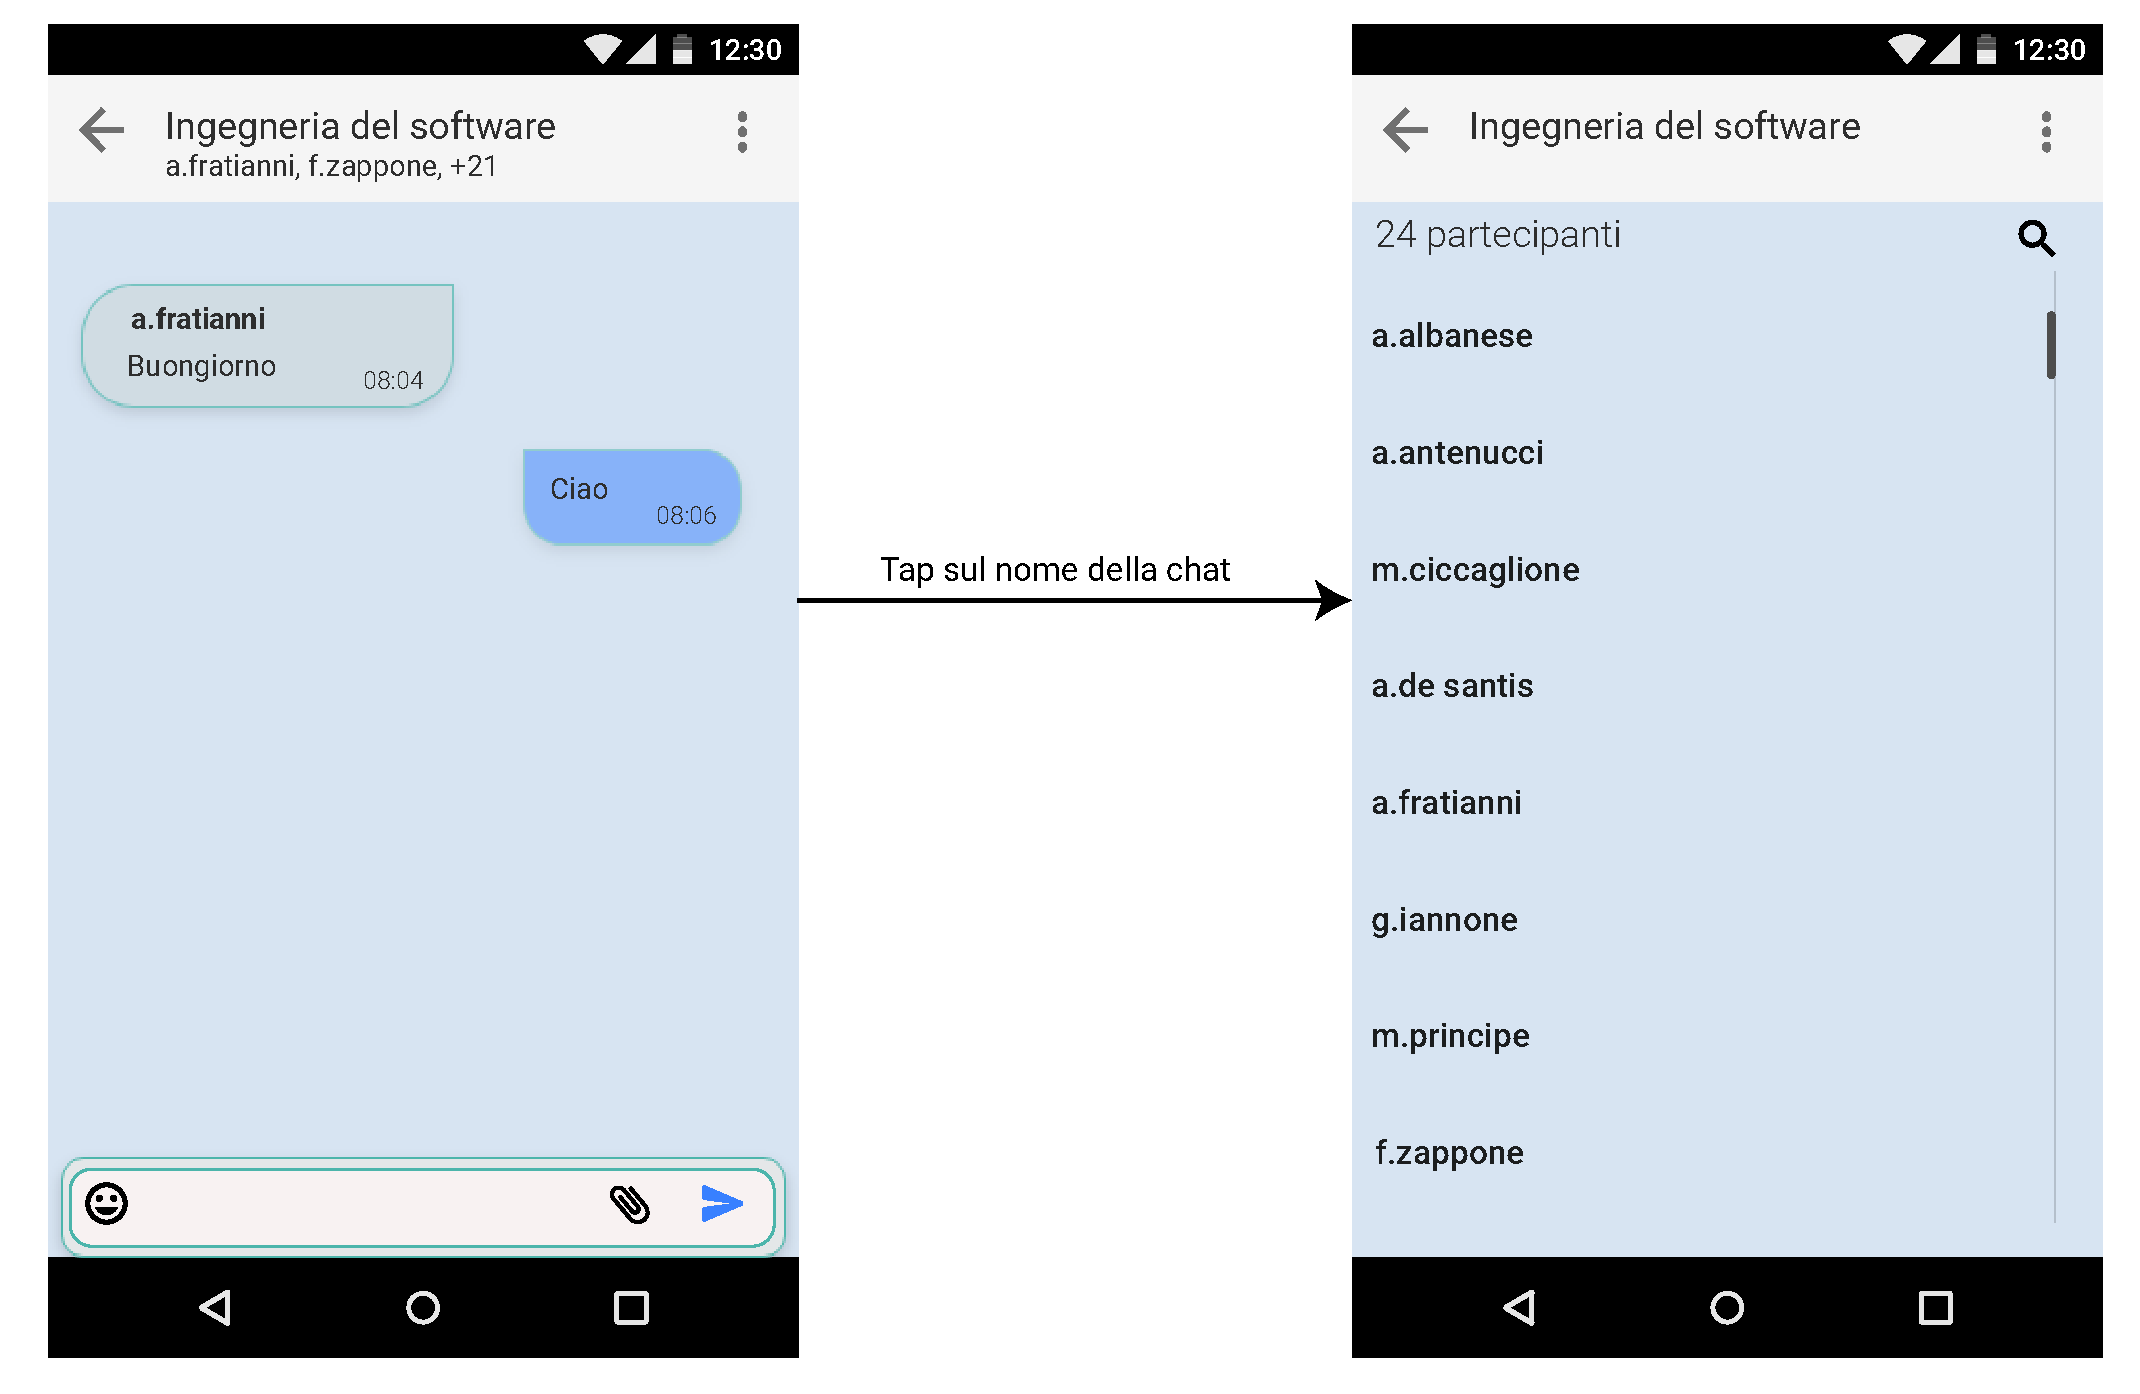
\includegraphics[width=0.9\textwidth]{imgs/gruppo6/activities/act_cus11_elenco_membri.pdf}
	\caption{CUS11 - Visualizza elenco membri chat}
	\label{fig:cus11}
\end{figure}
%%% END activities chat studenti %%%

%%% START activities chat docenti %%%
\pagebreak
\begin{figure}
\subsection{Activities relative alla chat dell'App Docenti}
	\centering
	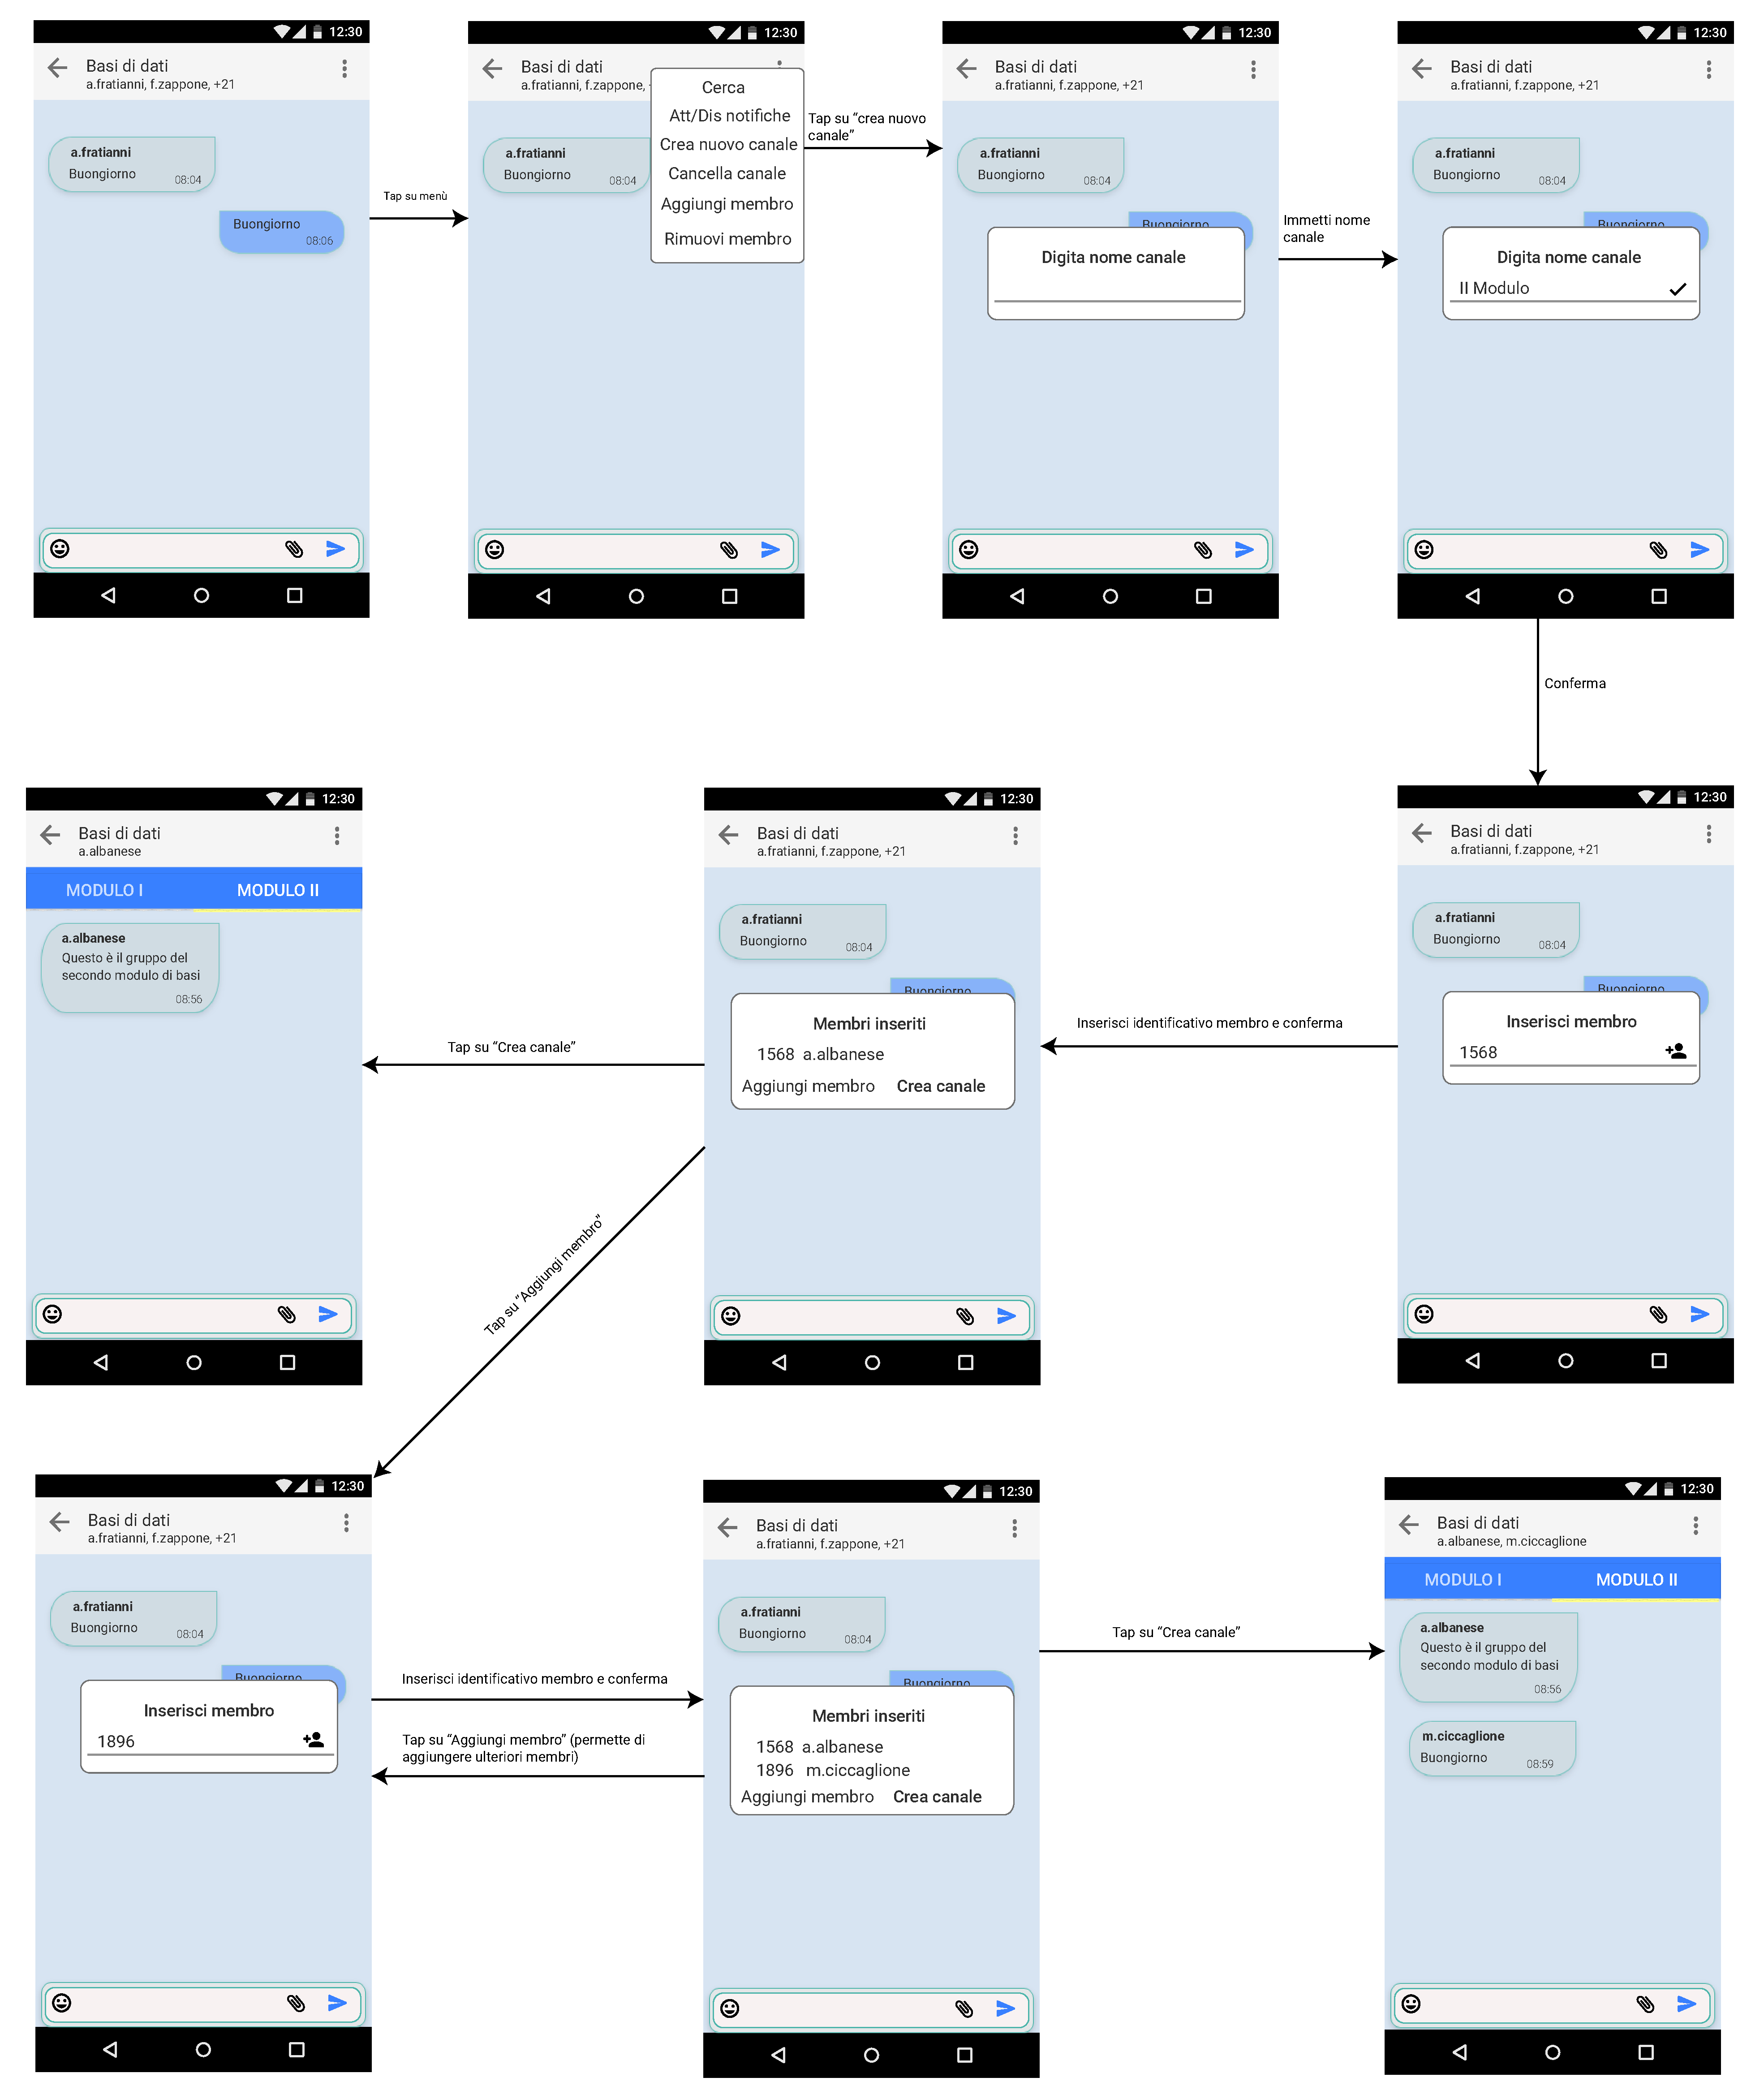
\includegraphics[width=0.9\textwidth]{imgs/gruppo6/activities/act_cud1_creazione_canale.pdf}
	\caption{CUD1 - Creazione canale}
	\label{fig:cud1}
\end{figure}

\begin{figure}
	\centering
	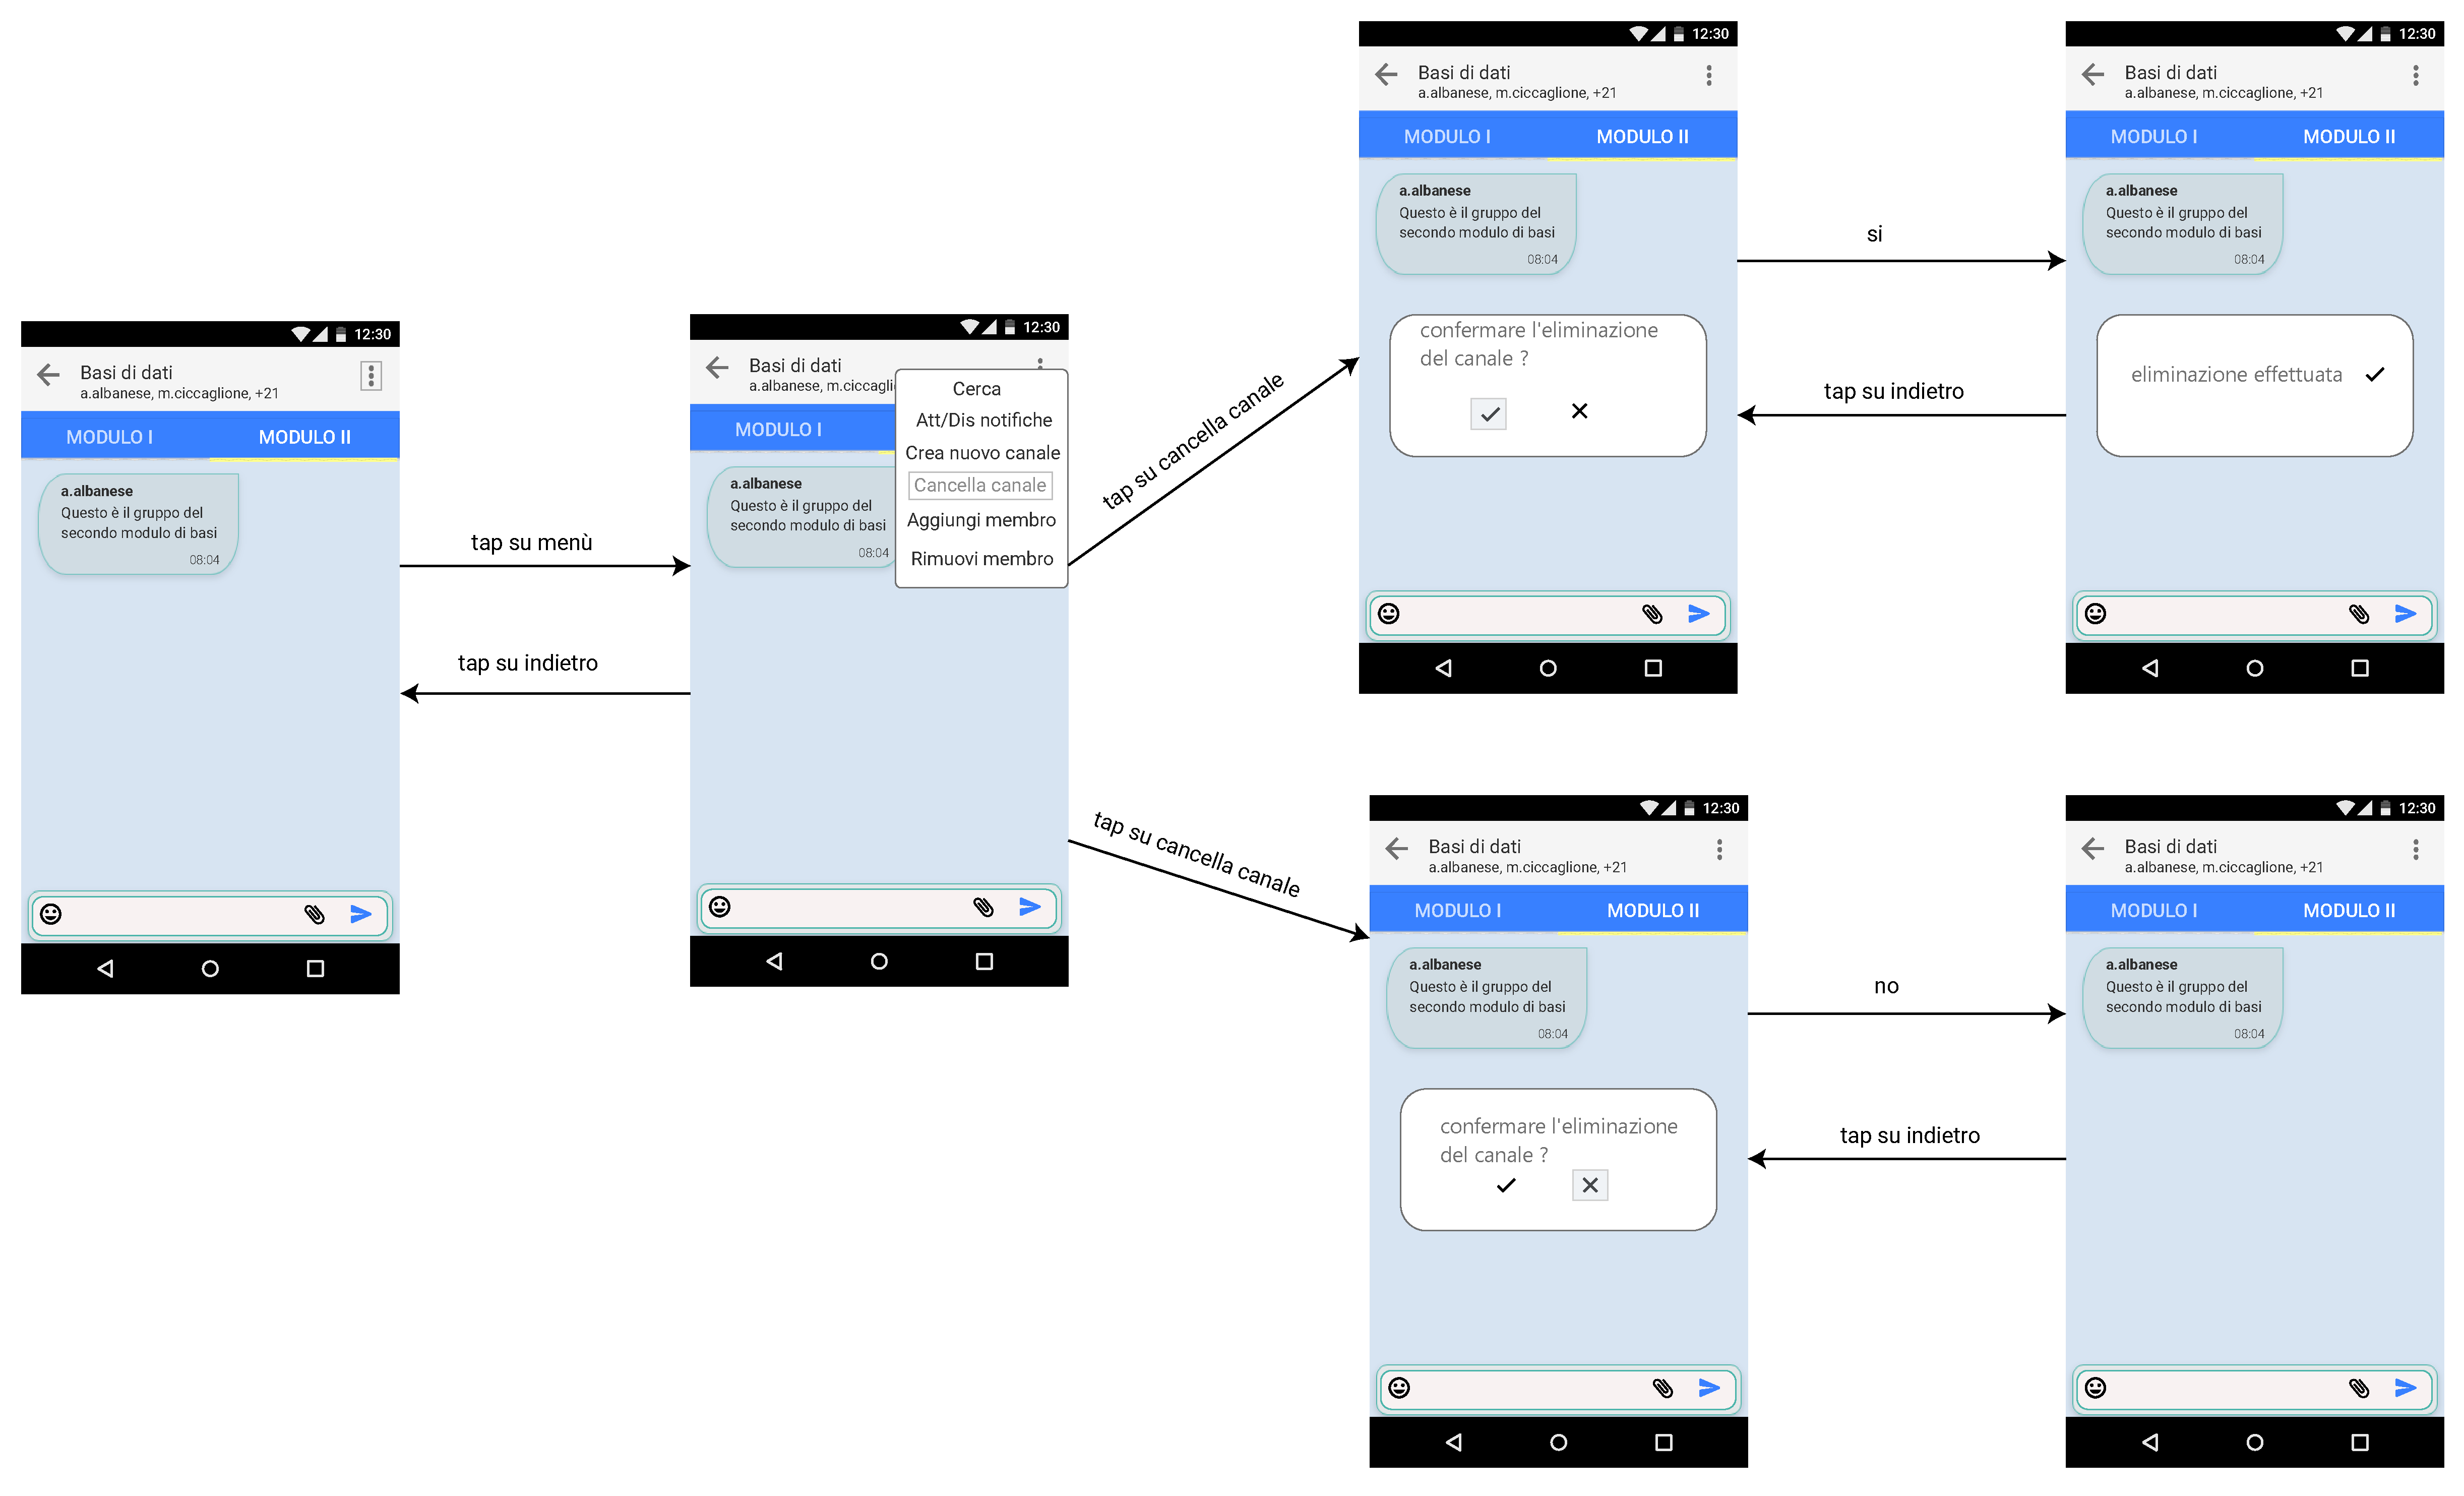
\includegraphics[width=0.9\textwidth]{imgs/gruppo6/activities/act_cud2_cancella_canale.pdf}
	\caption{CUD2 - Cancellazione canale}
	\label{fig:cud2}
\end{figure}

\begin{figure}
	\centering
	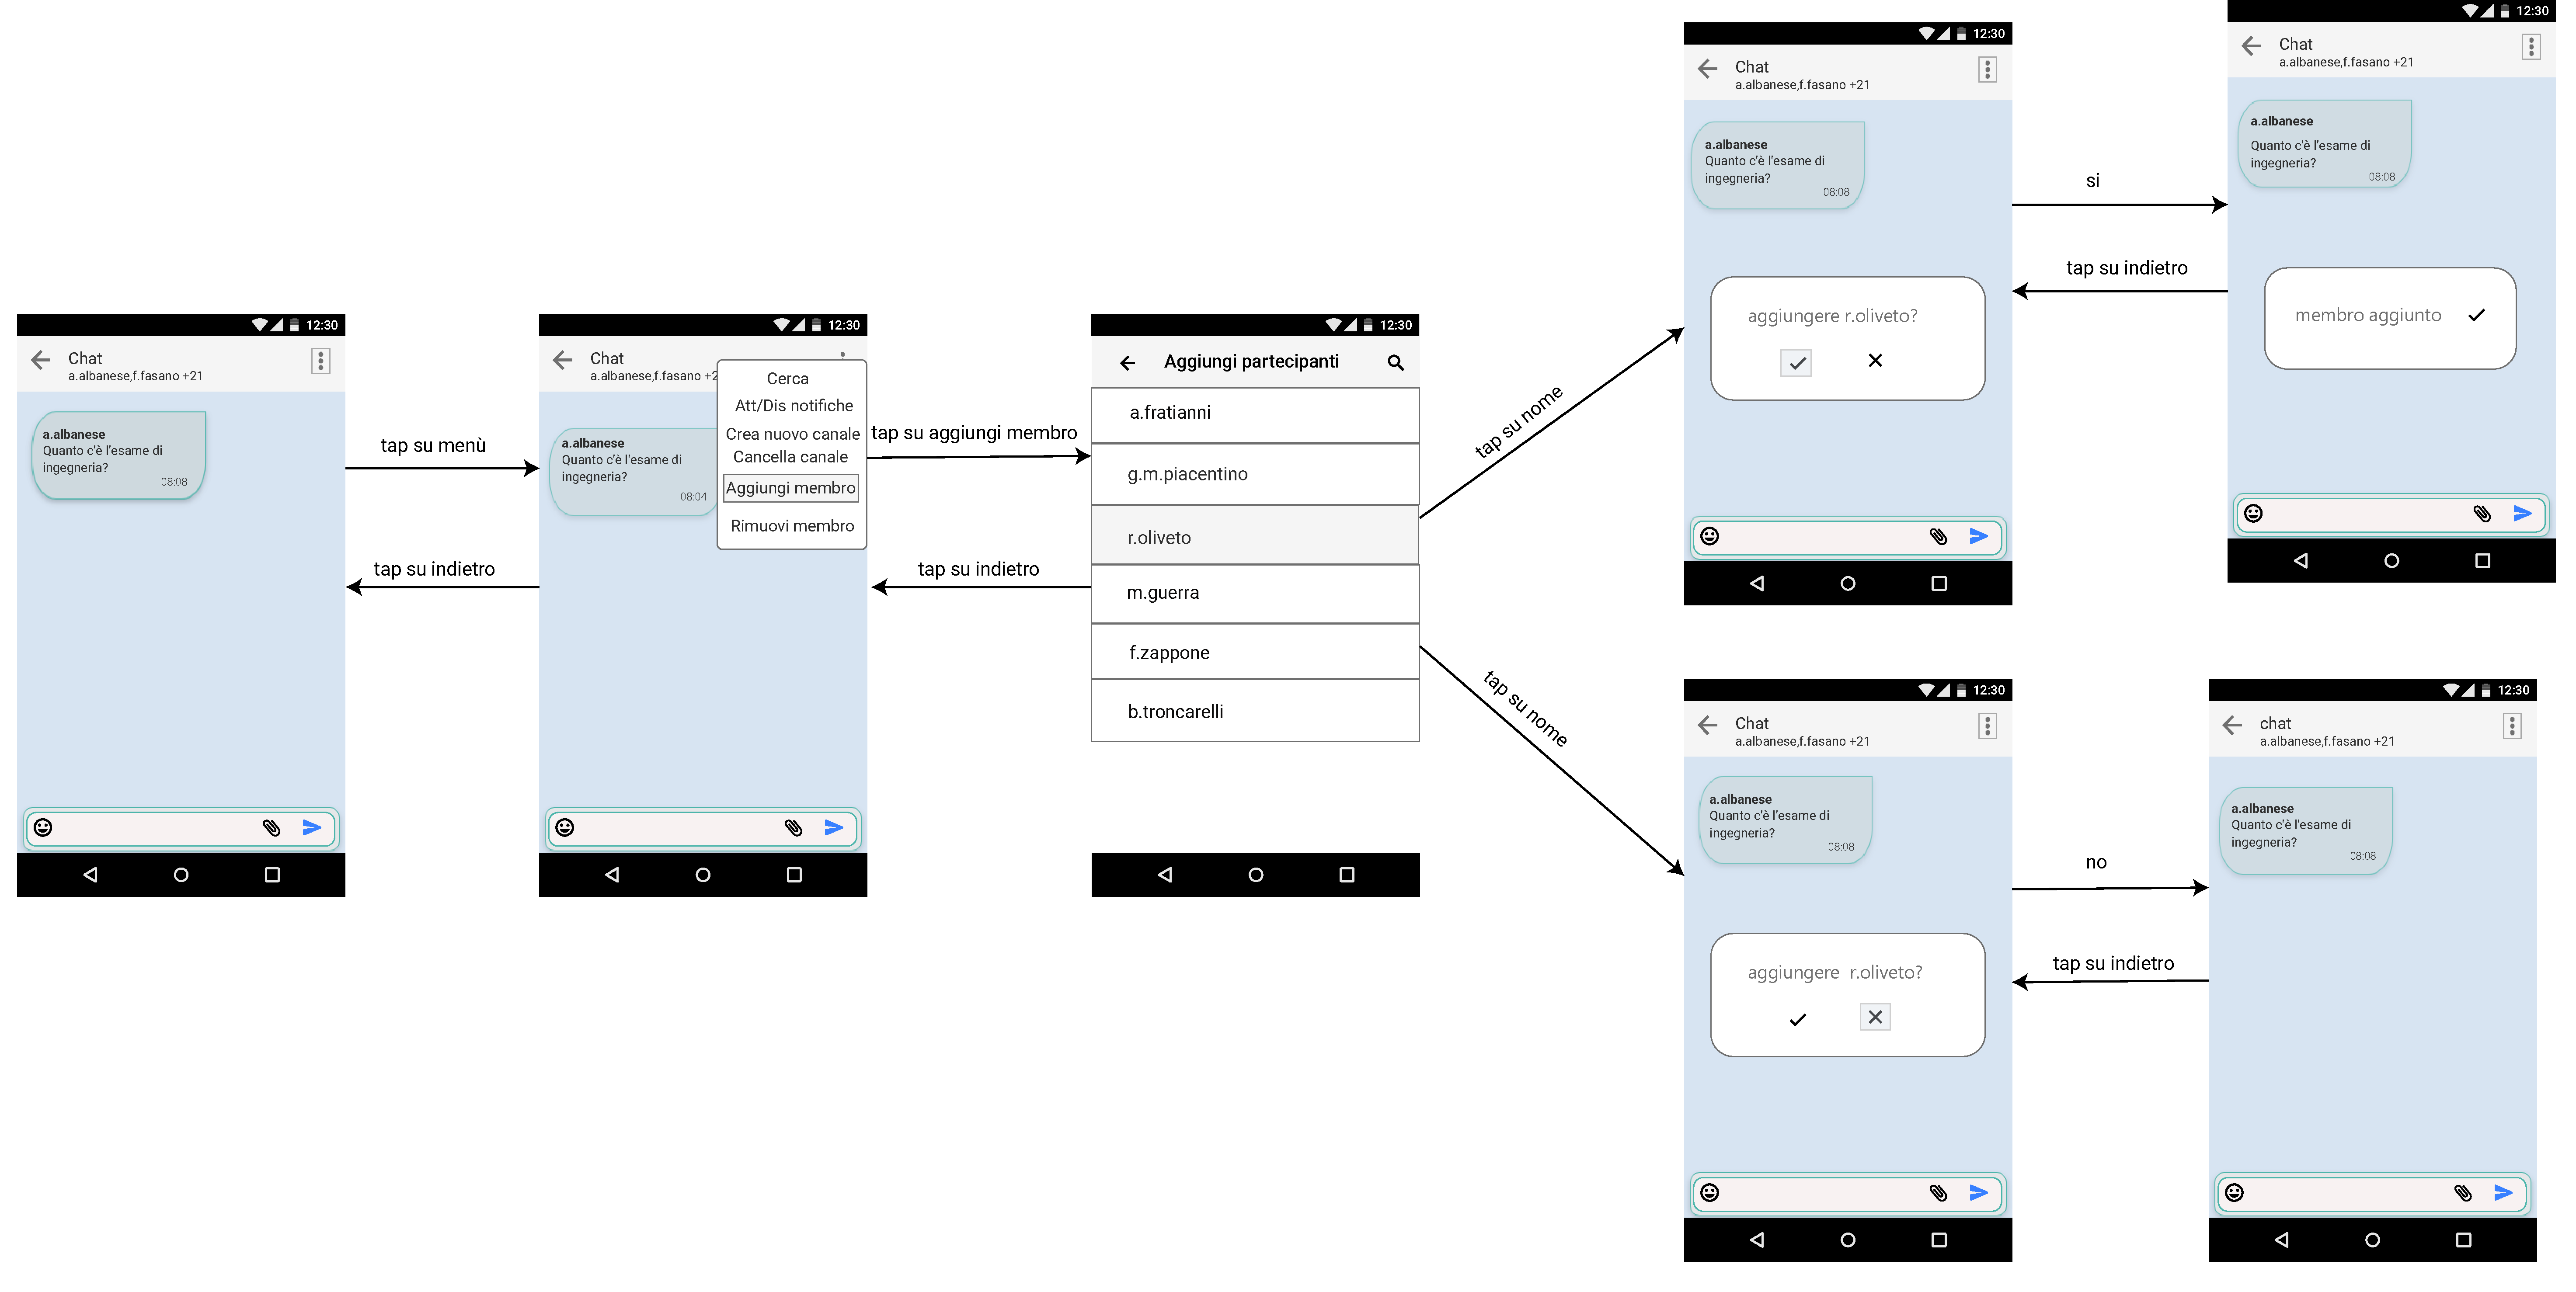
\includegraphics[width=0.9\textwidth]{imgs/gruppo6/activities/act_cud3_aggiungi_membro_chat.pdf}
	\caption{CUD3 - Aggiungi membro ad un canale}
	\label{fig:cud3}
\end{figure}

\begin{figure}
	\centering
	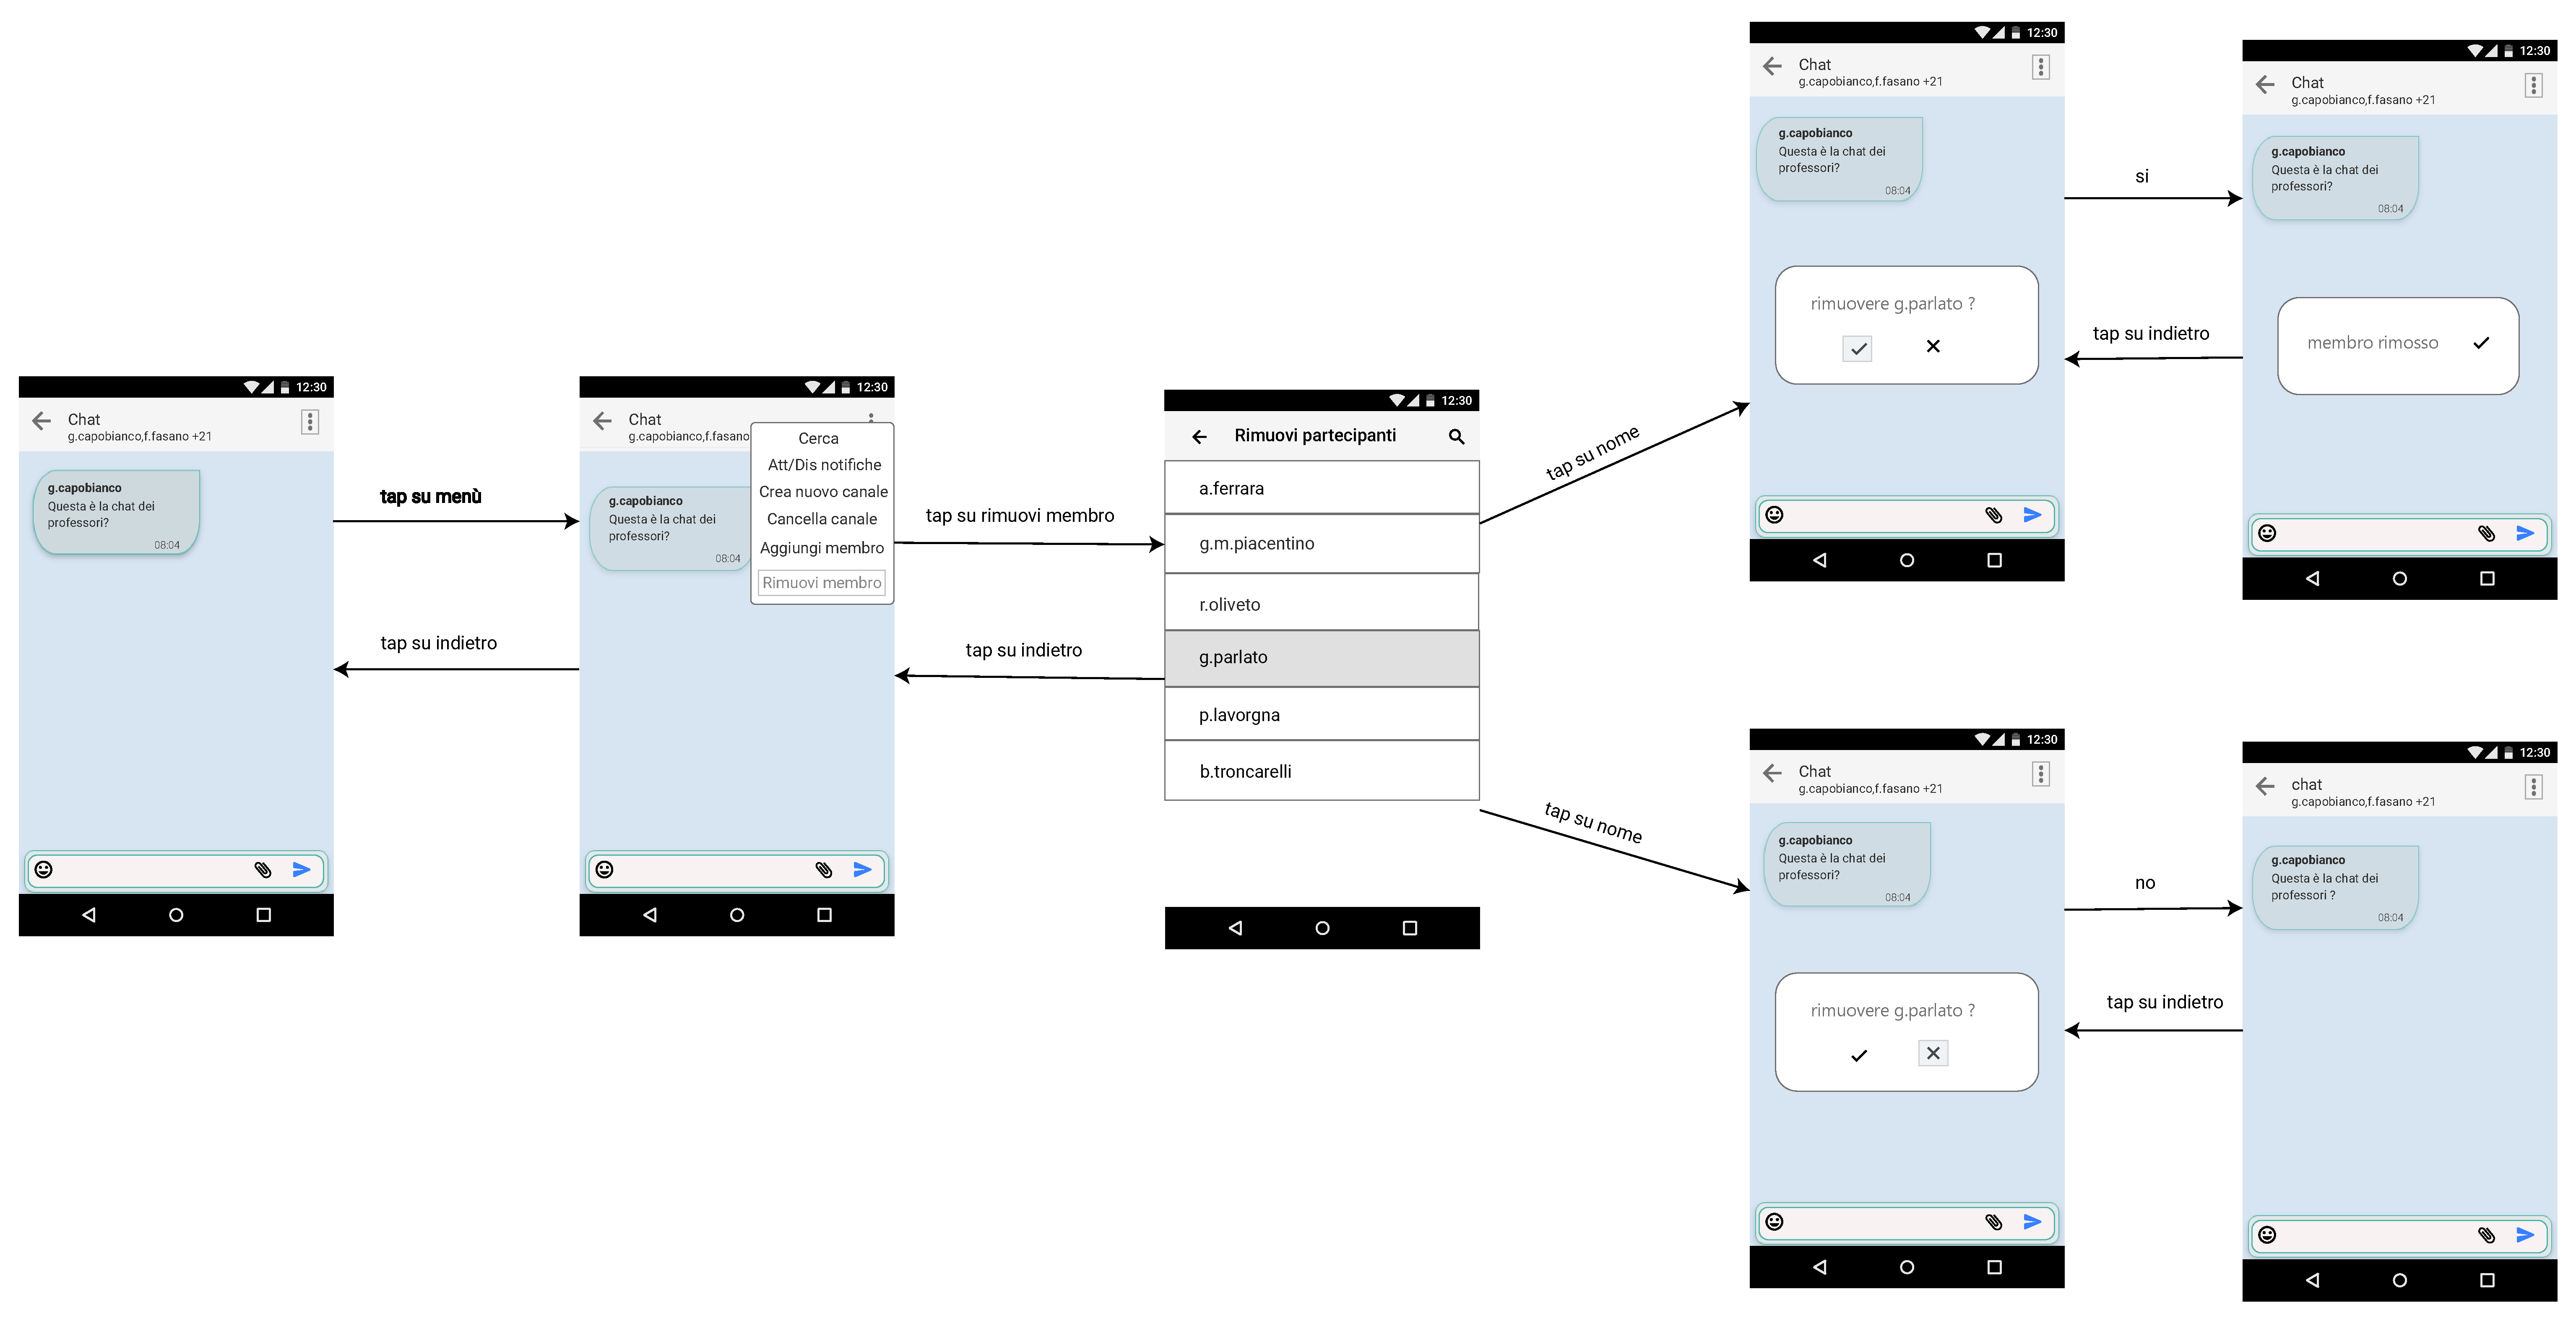
\includegraphics[width=0.9\textwidth]{imgs/gruppo6/activities/act_cud4_rimuovi_membro_da_canale.pdf}
	\caption{CUD4 - Rimuovi membro da un canale}
	\label{fig:cud4}
\end{figure}

\begin{figure}
	\centering
	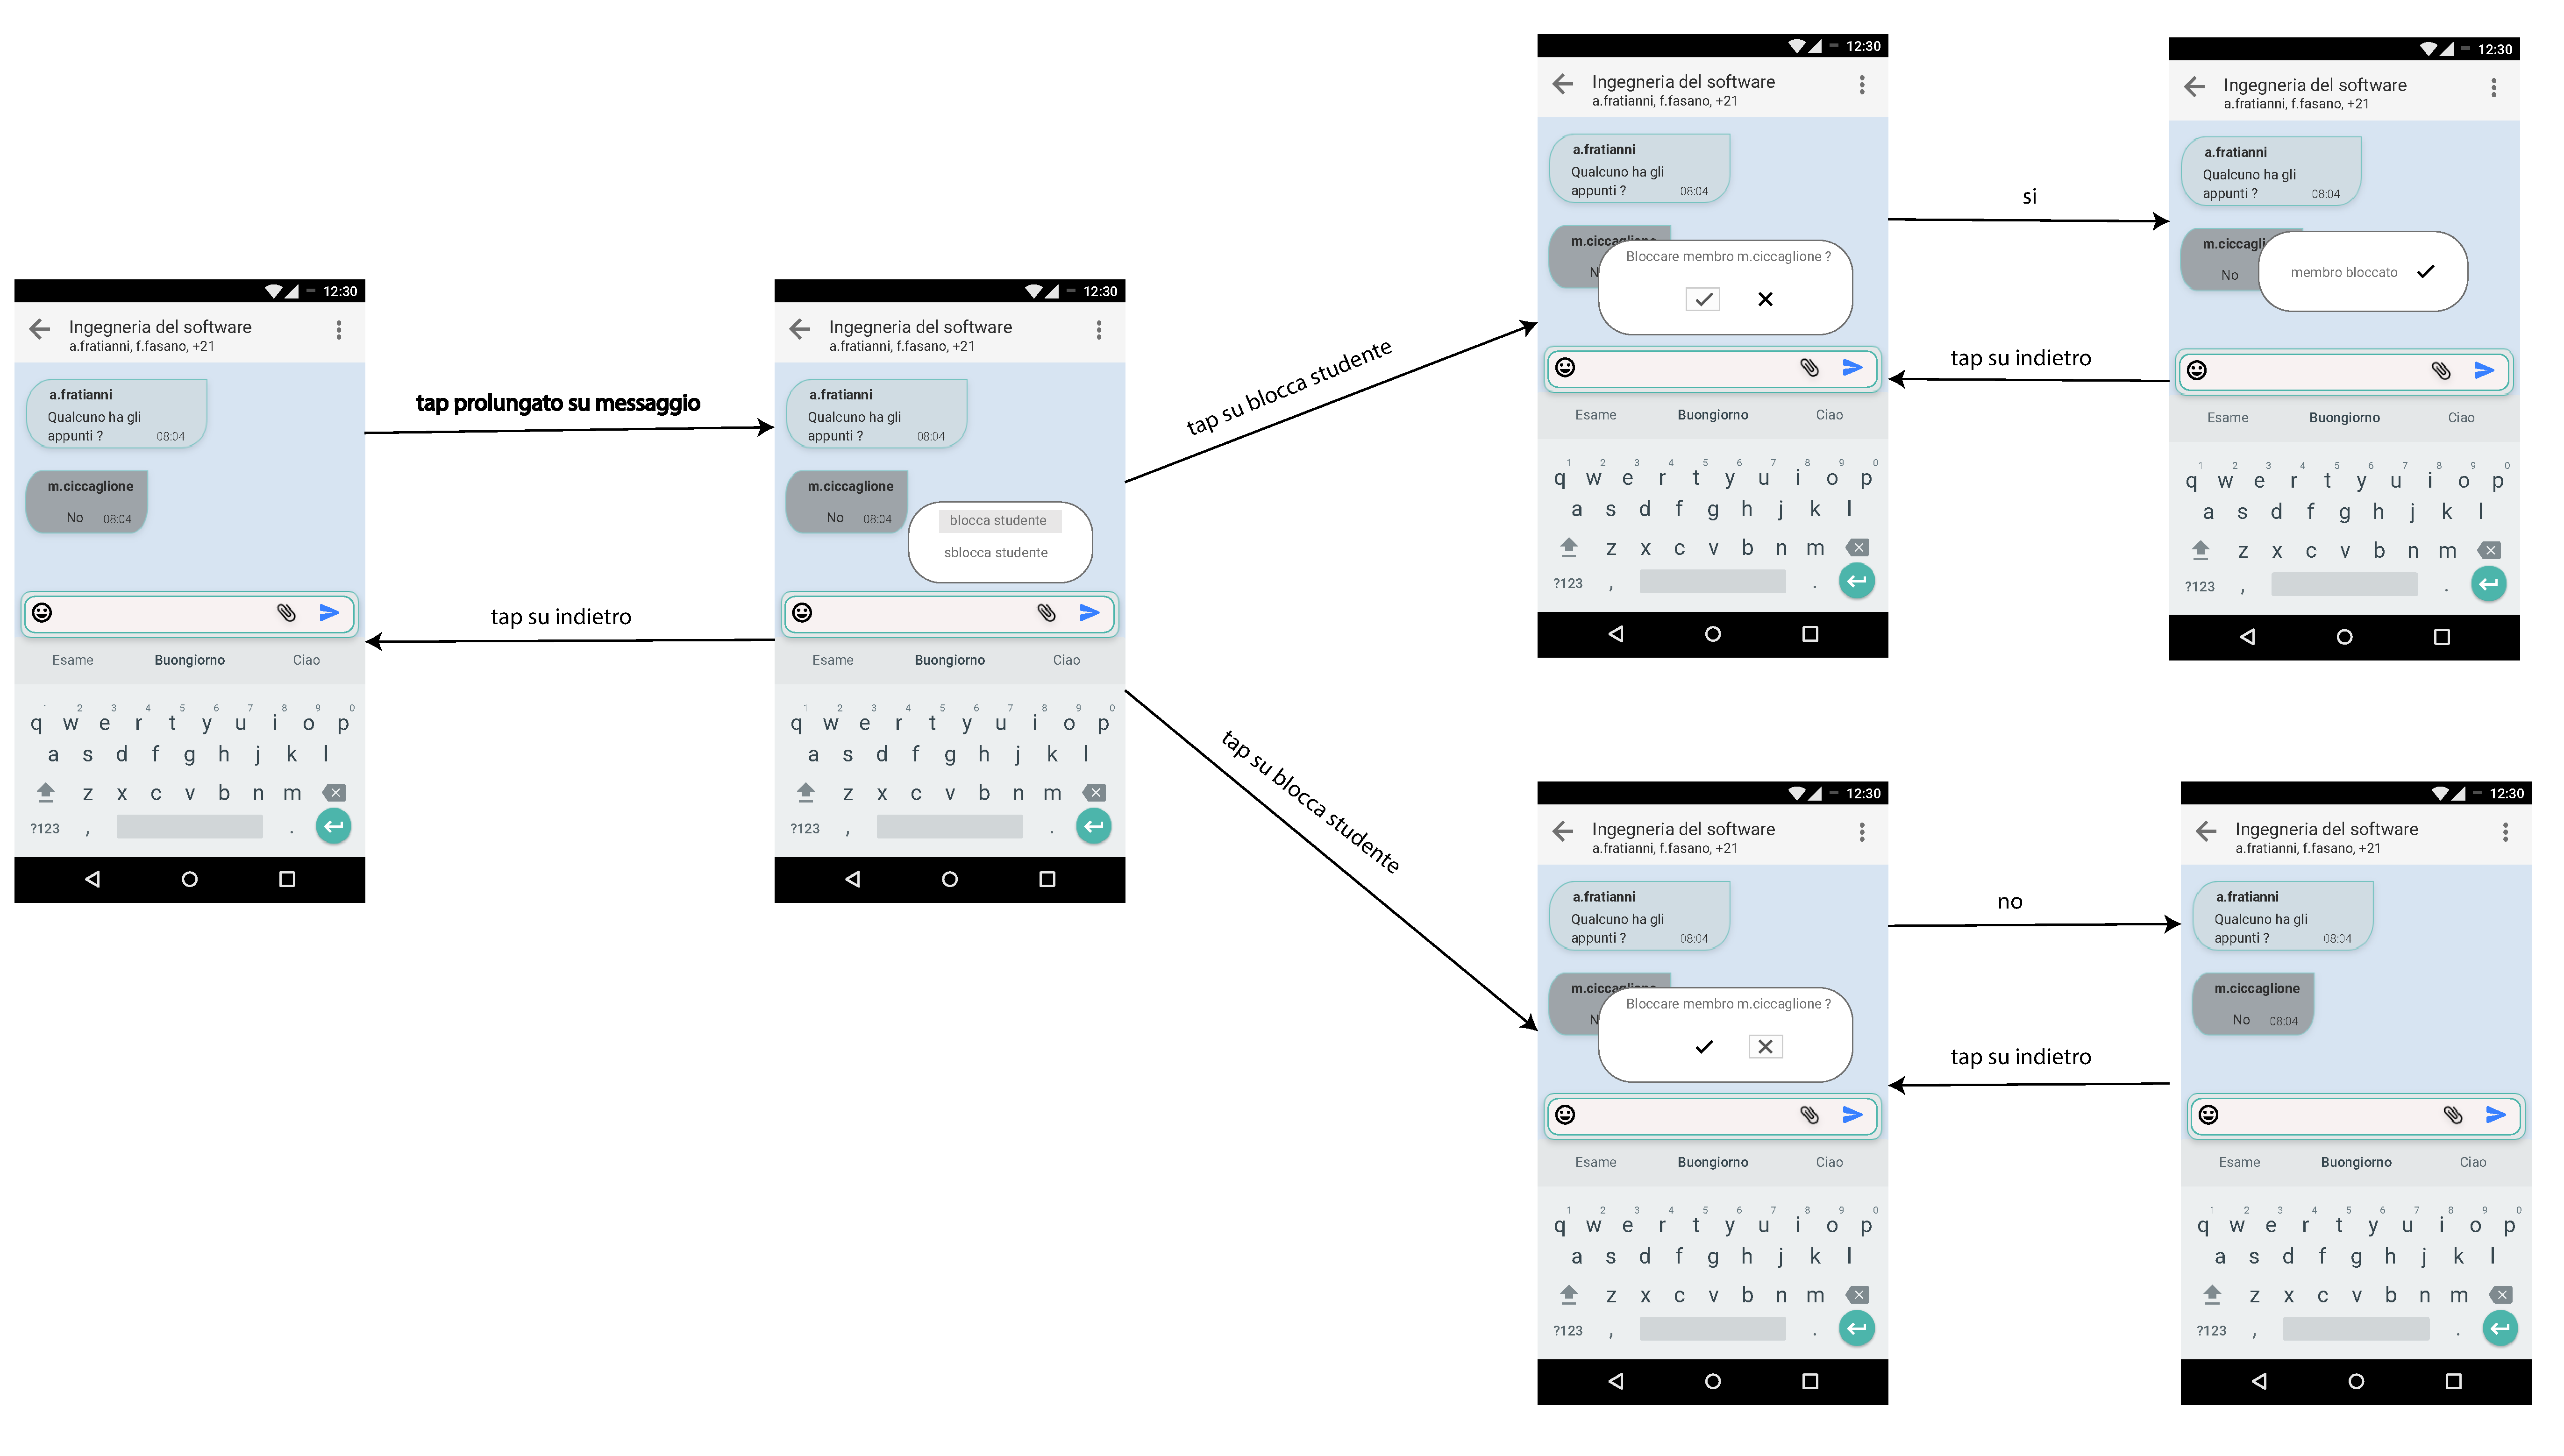
\includegraphics[width=0.9\textwidth]{imgs/gruppo6/activities/act_cud5_blocca_studente.pdf}
	\caption{CUD5 - Blocca Studente}
	\label{fig:cud5}
\end{figure}

\begin{figure}
	\centering
	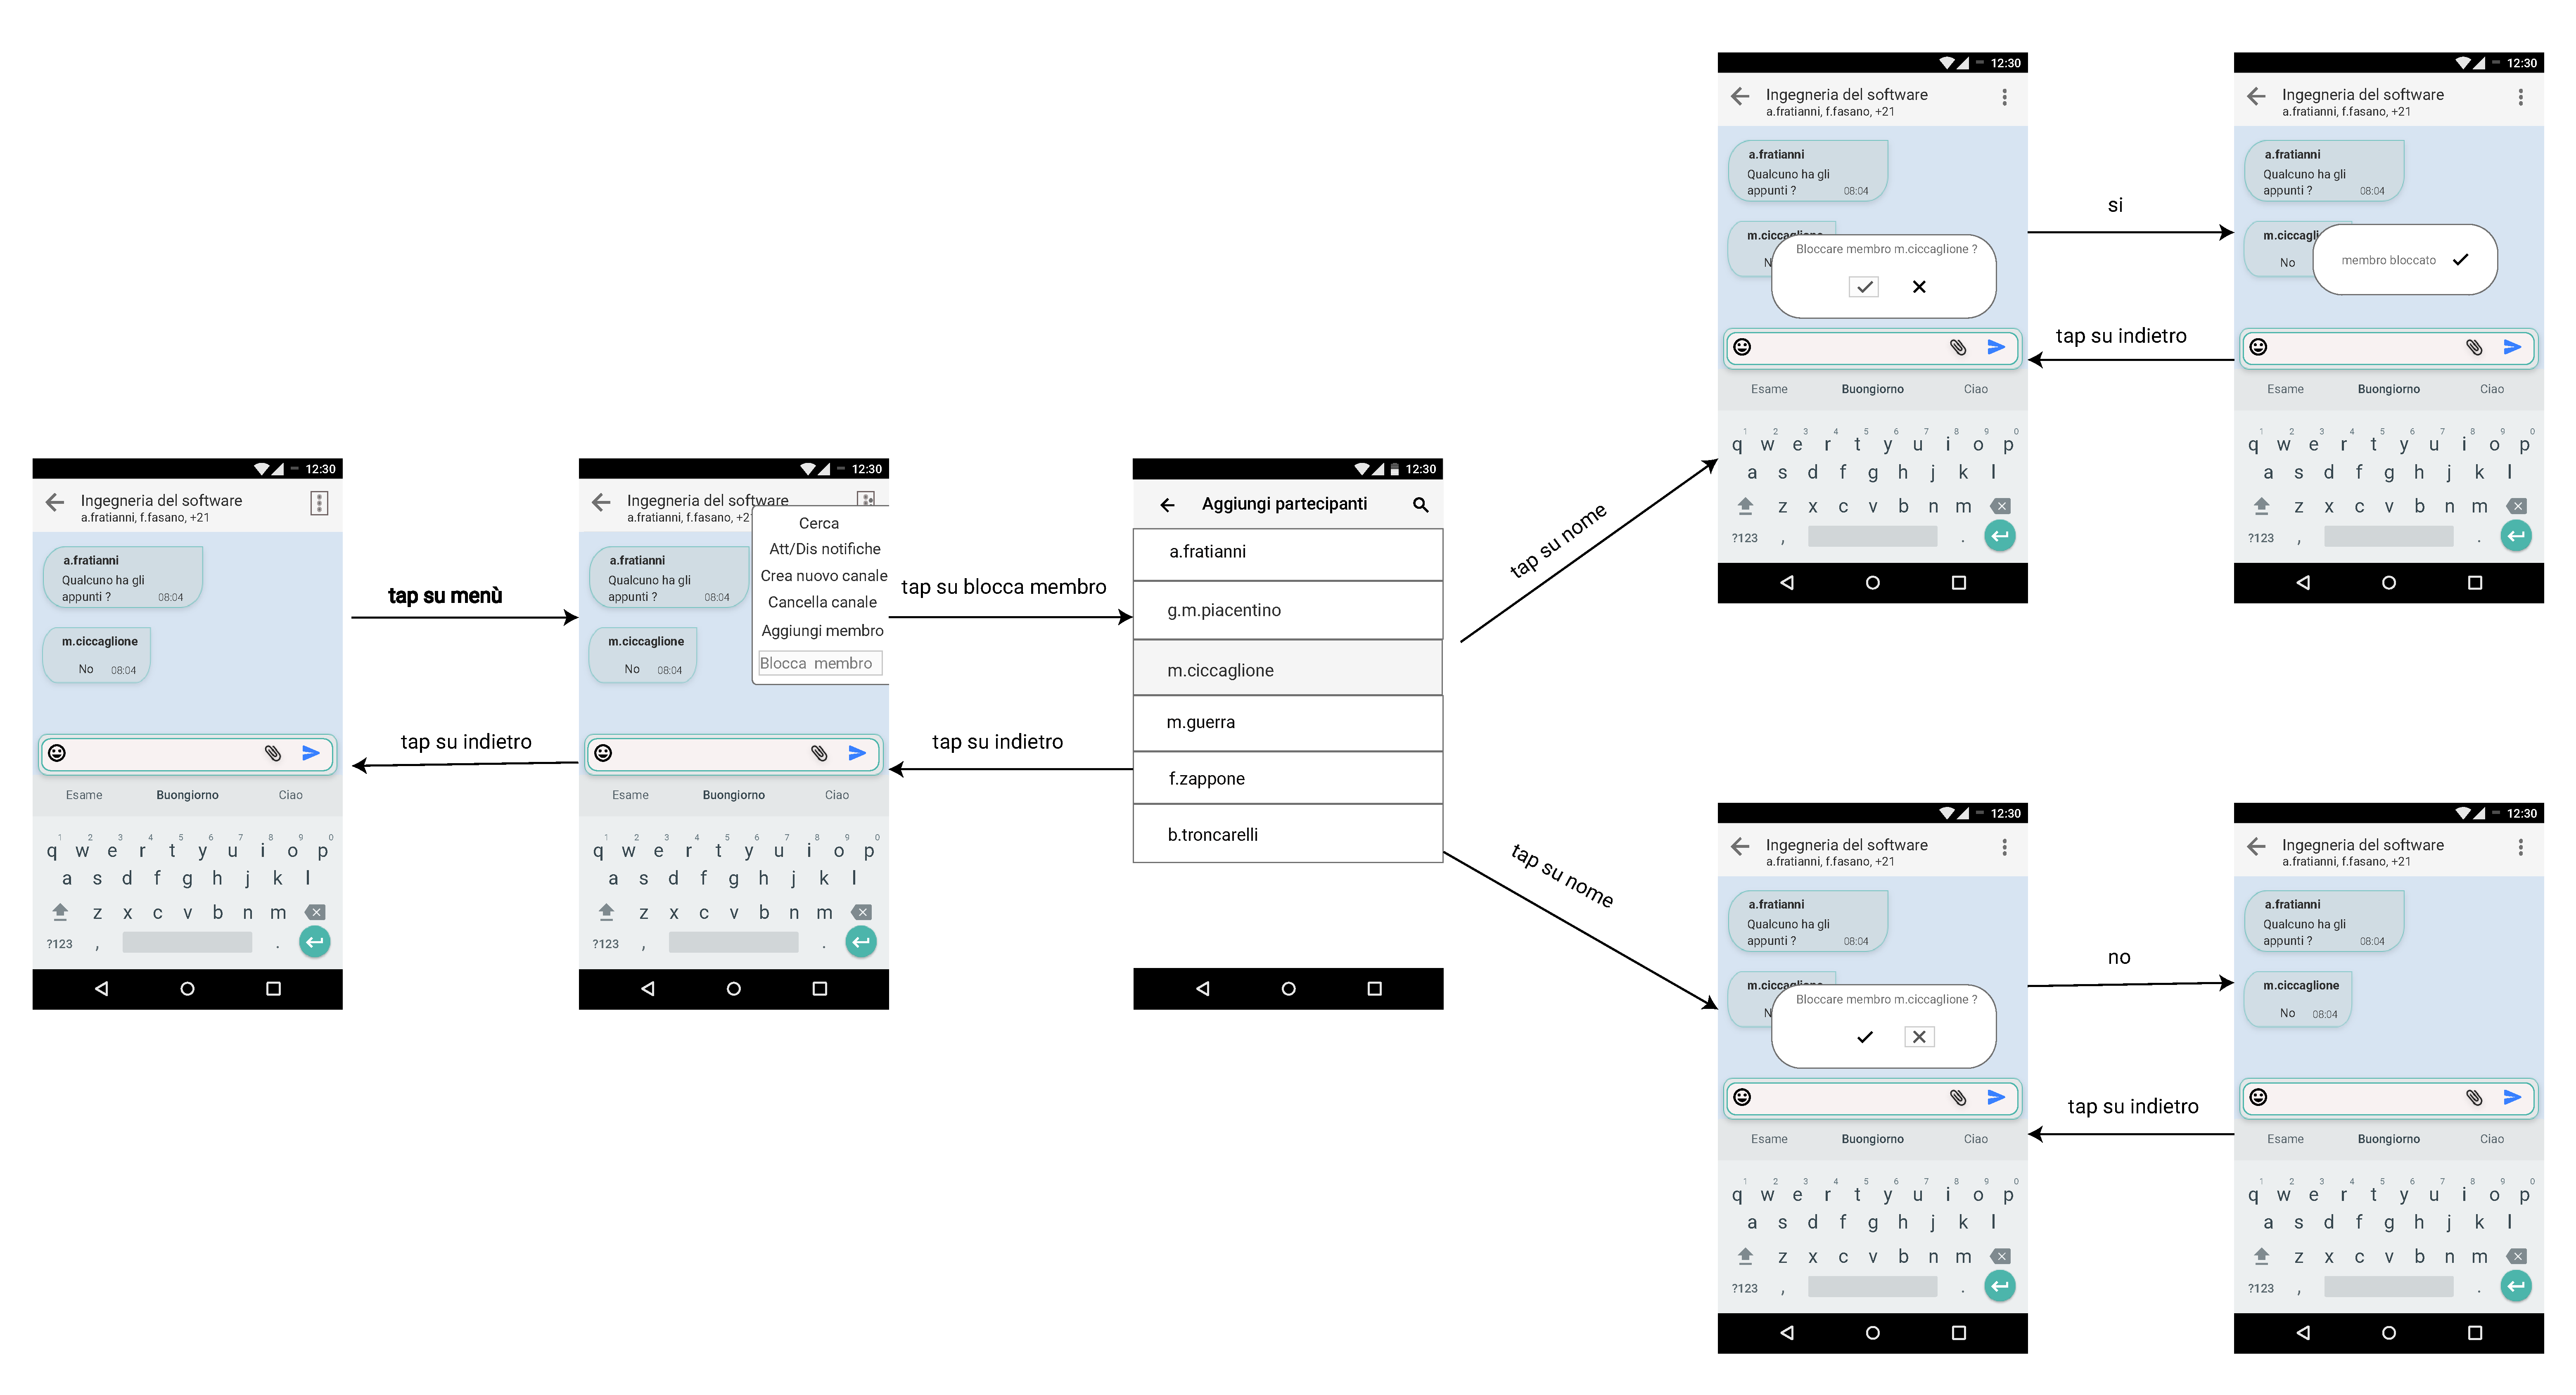
\includegraphics[width=0.9\textwidth]{imgs/gruppo6/activities/act_cud5_blocca_studente2.pdf}
	\caption{CUD5 - Blocca Studente (es. 2}
	\label{fig:cud5-2}
\end{figure}

\begin{figure}
	\centering
	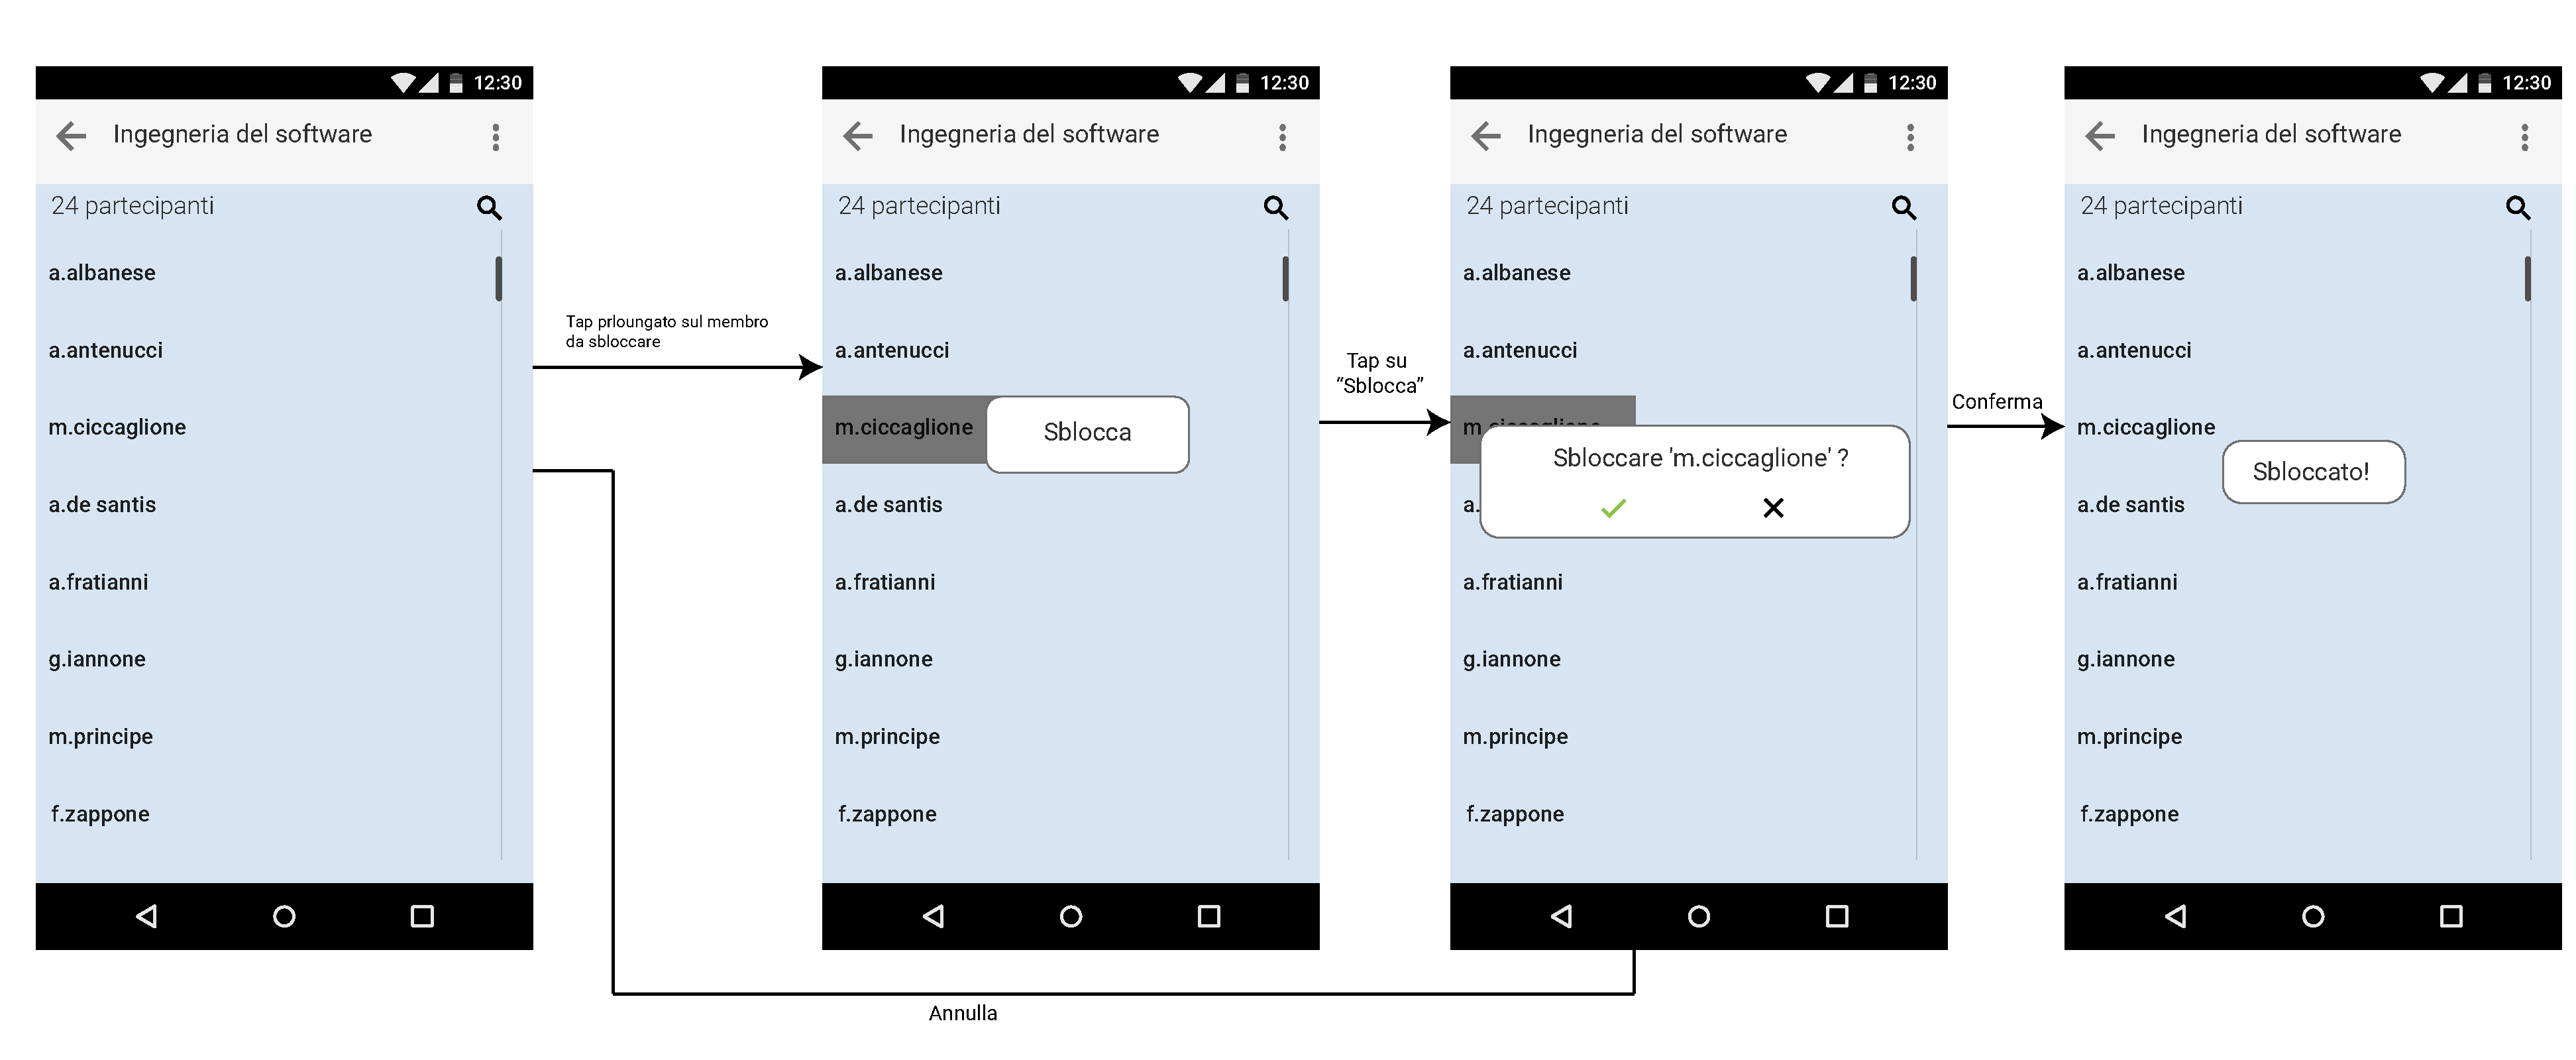
\includegraphics[width=0.9\textwidth]{imgs/gruppo6/activities/act_cud6_sblocca_da_elenco.pdf}
	\caption{CUD6 - Sblocca Studente (da elenco)}
	\label{fig:cud6}
\end{figure}

\begin{figure}
	\centering
	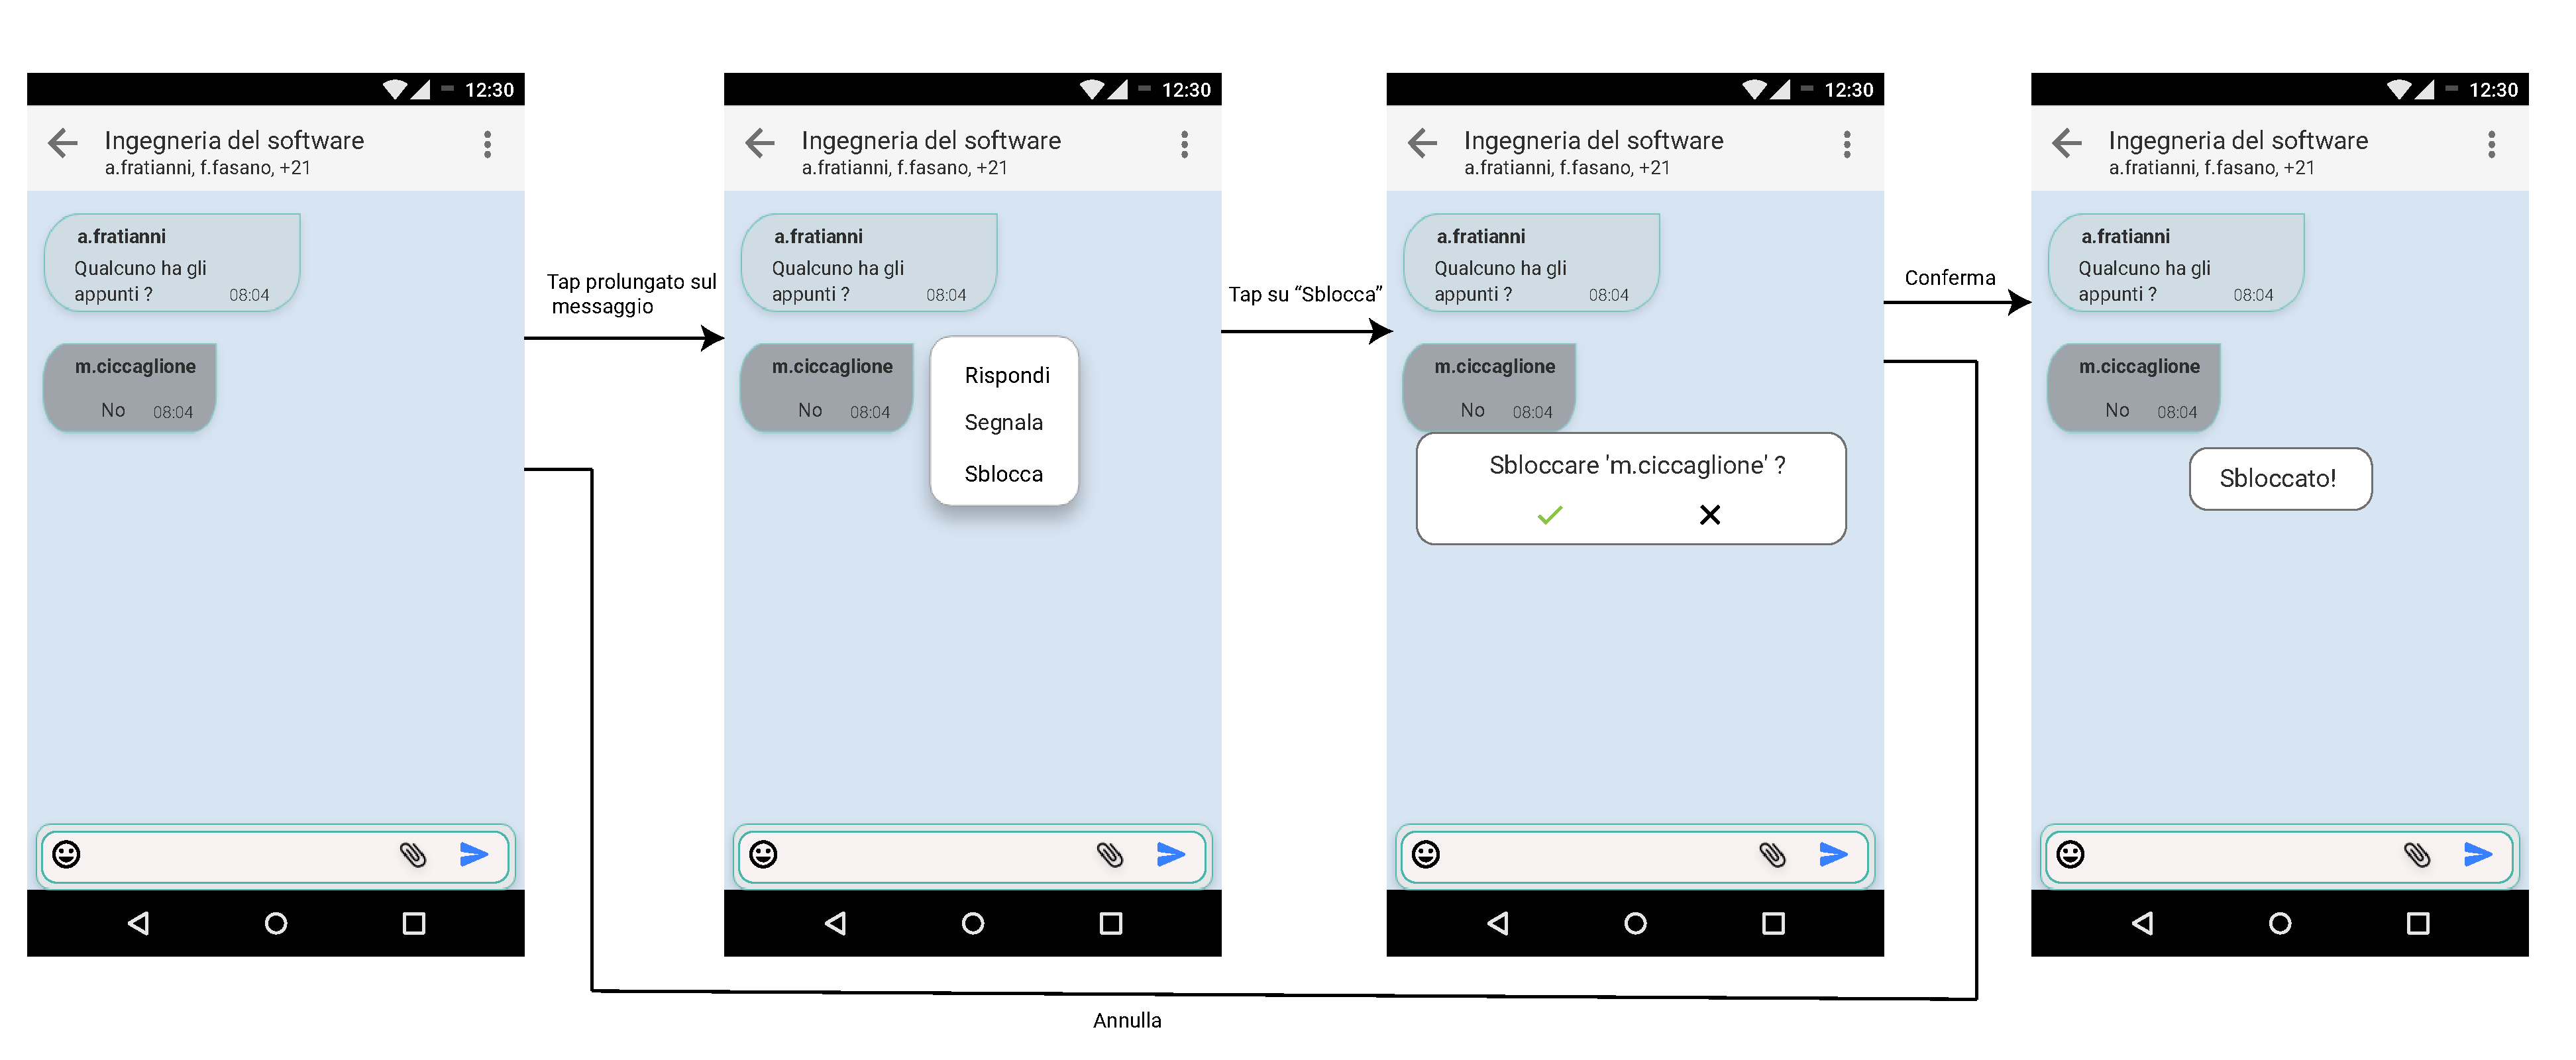
\includegraphics[width=0.9\textwidth]{imgs/gruppo6/activities/act_cud6_sblocca_da_messaggio.pdf}
	\caption{CUD6 - Sblocca Studente (da messaggio)}
	\label{fig:cud6}
\end{figure}
%%% END activities chat docenti %%%

%%% START activities chat pannello %%%
\pagebreak
\begin{figure}
\subsection{Activities relative al pannello di amministrazione}
	\centering
	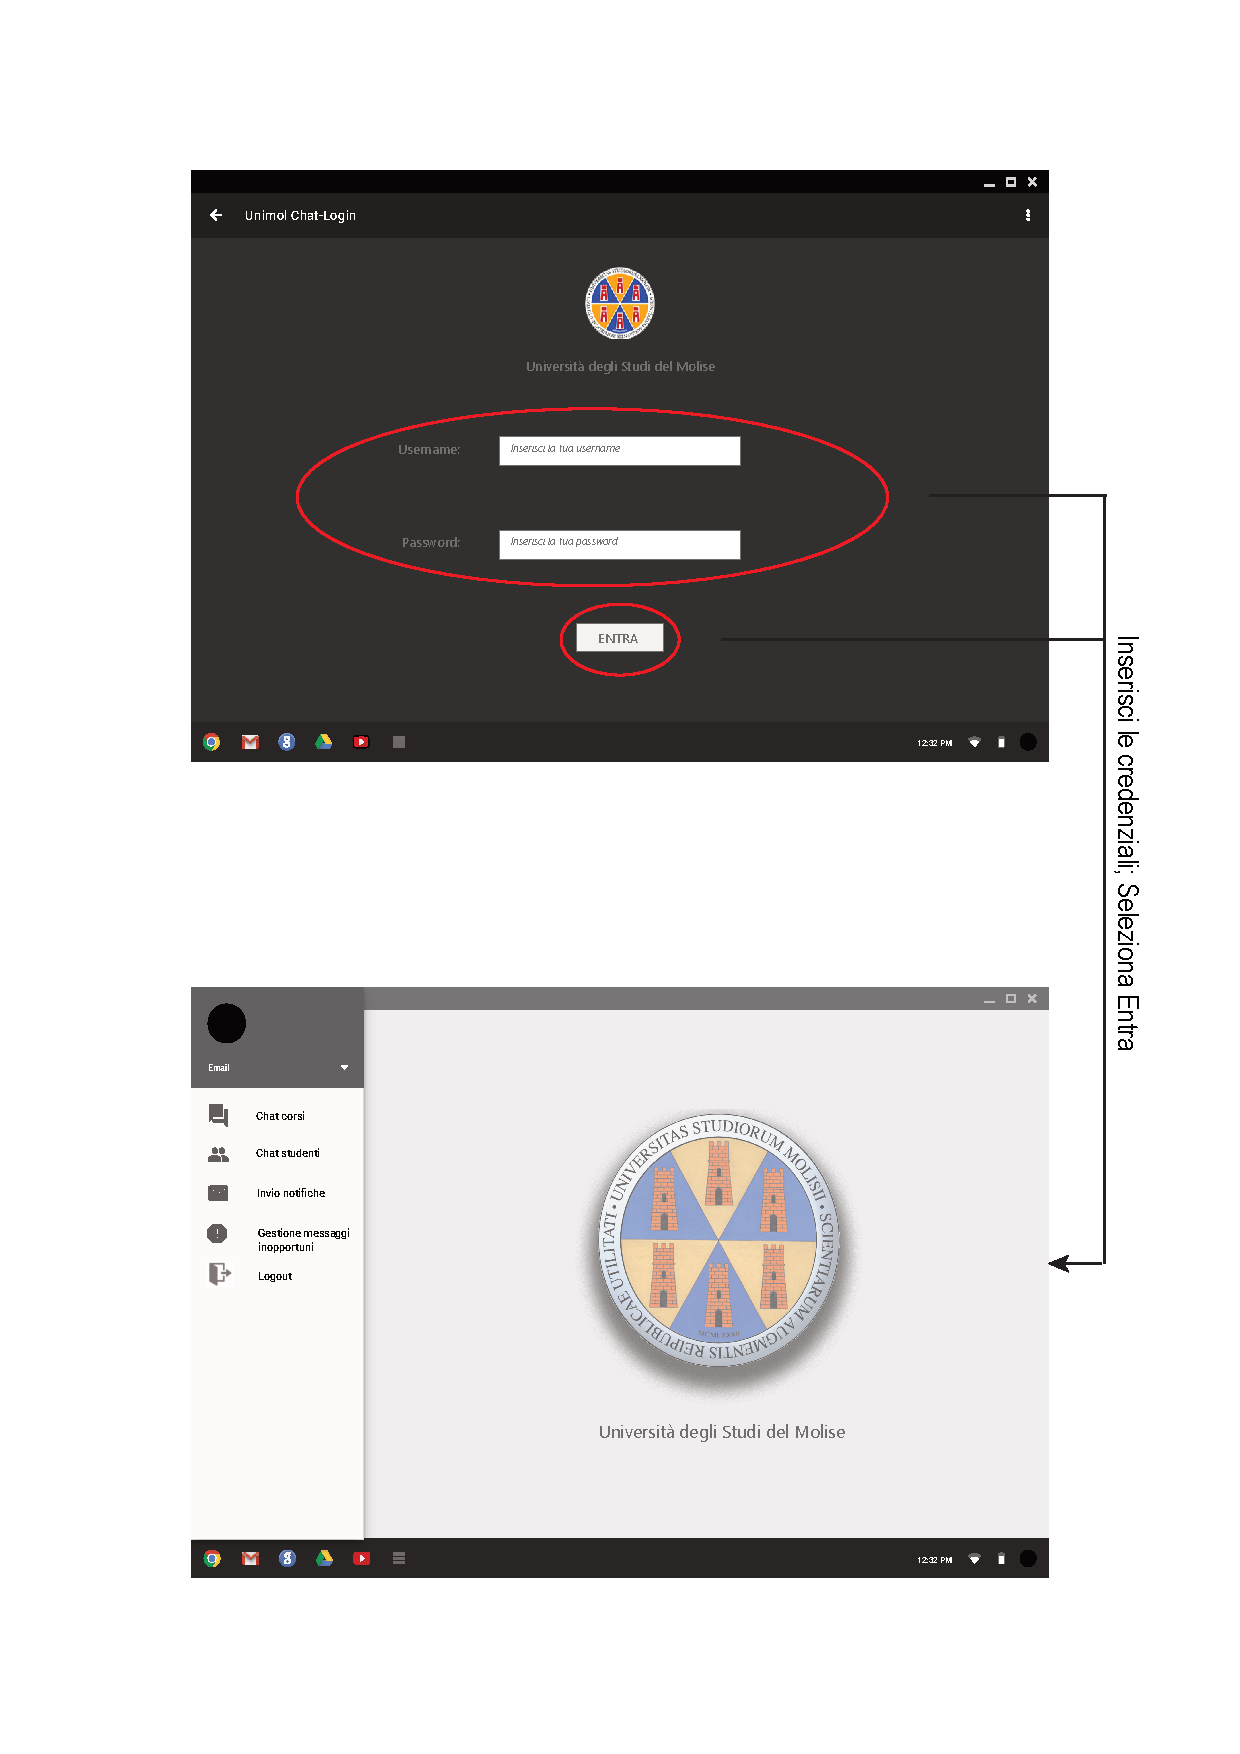
\includegraphics[width=0.9\textwidth]{imgs/gruppo6/activities/act_cup1_login.pdf}
	\caption{CUP1 - Login}
	\label{fig:cup1}
\end{figure}

\begin{figure}
	\centering
	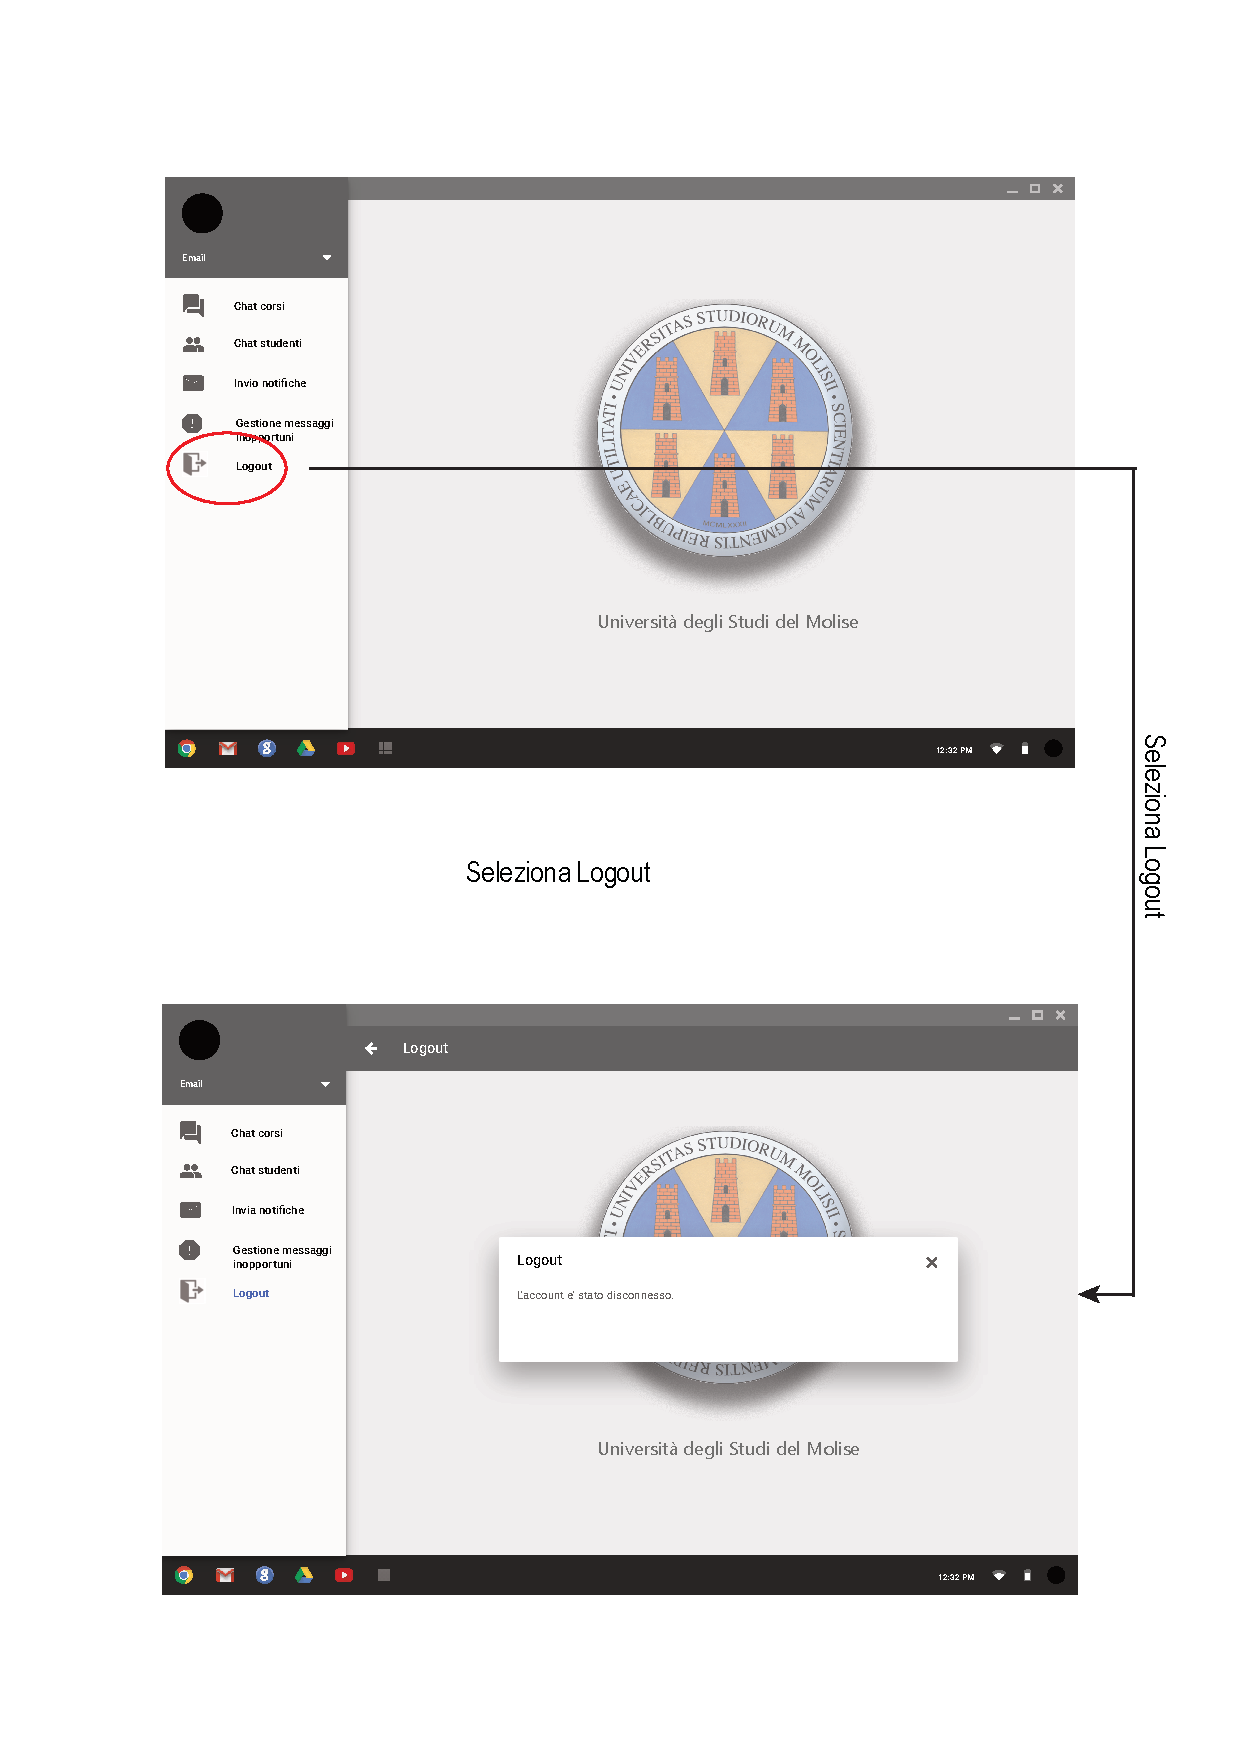
\includegraphics[width=0.9\textwidth]{imgs/gruppo6/activities/act_cup2_logout.pdf}
	\caption{CUP2 - Logout}
	\label{fig:cup2}
\end{figure}

\begin{figure}
	\centering
	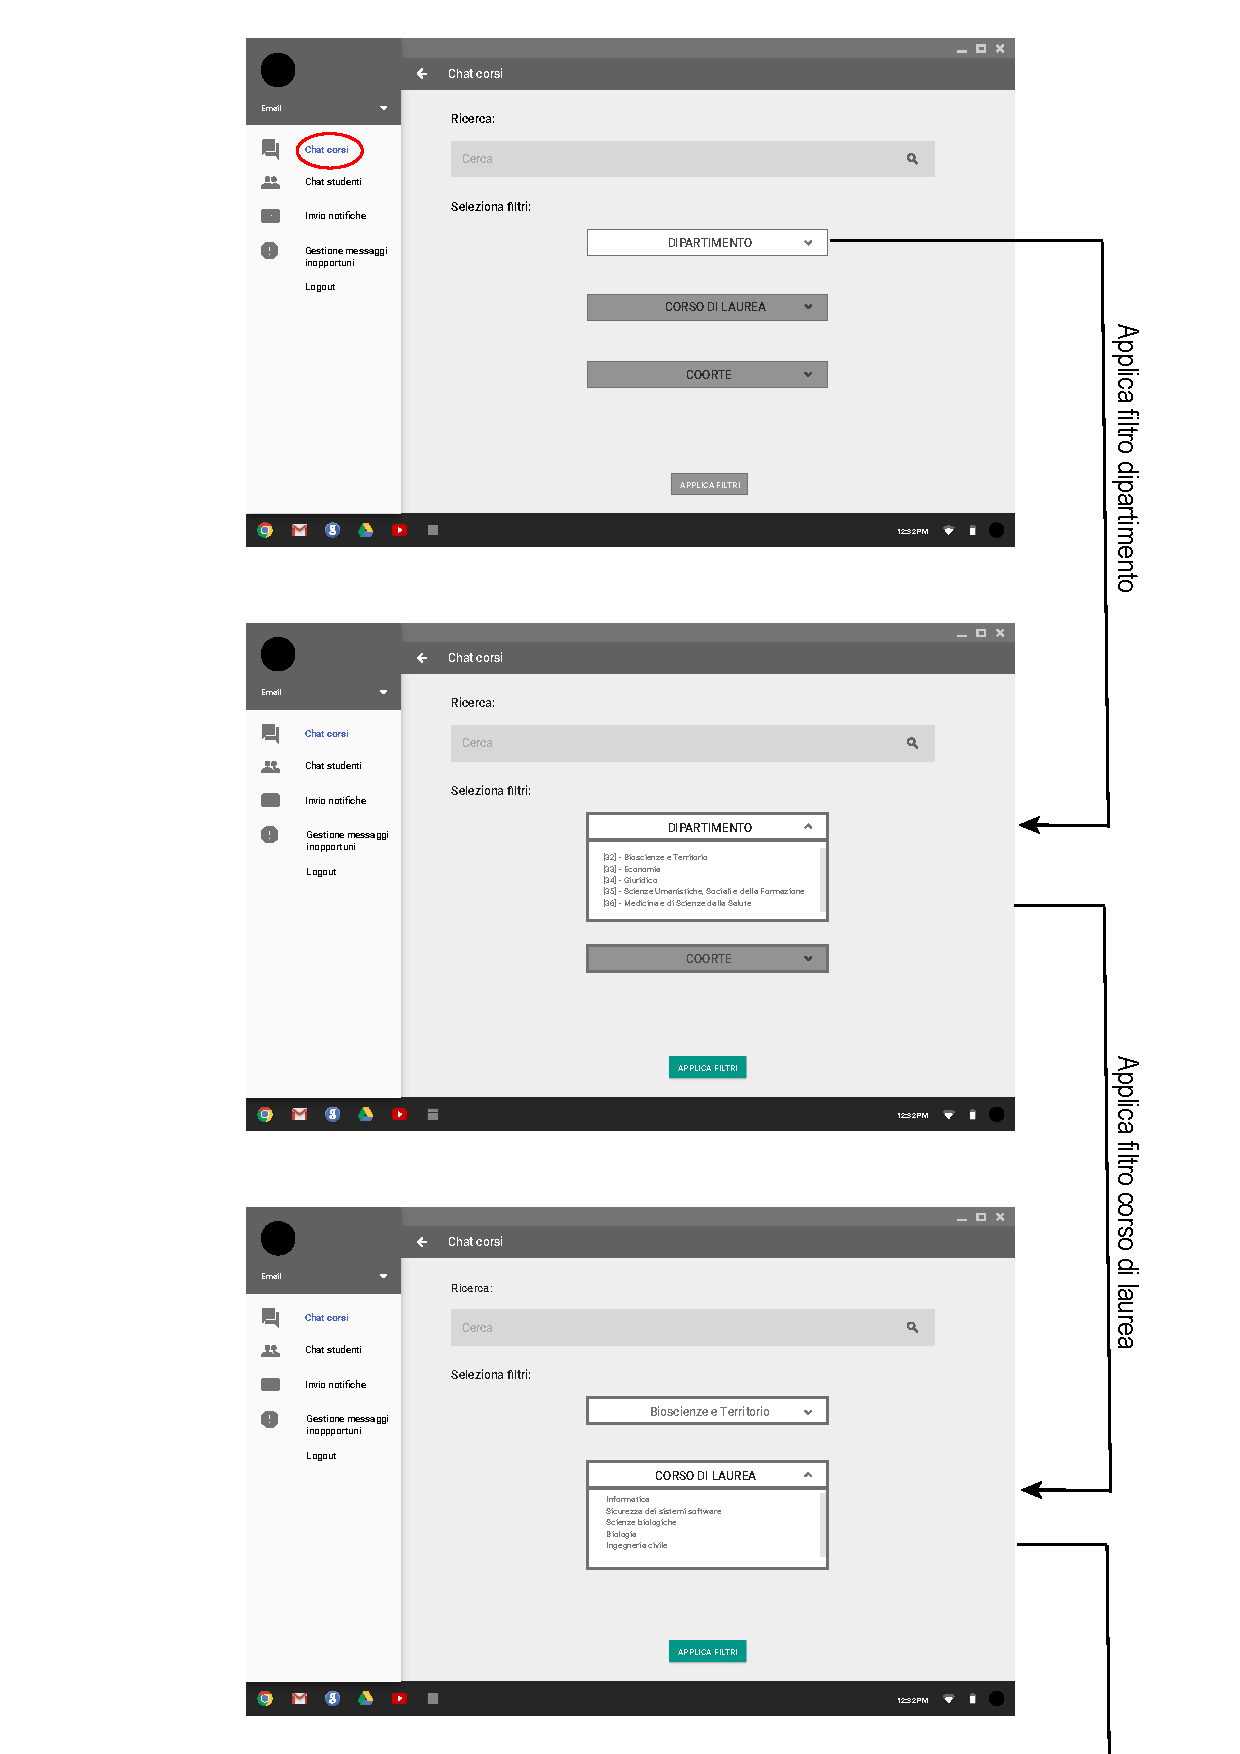
\includegraphics[width=0.9\textwidth]{imgs/gruppo6/activities/act_cup3_filtro_chat_corsi1.pdf}
	\caption{CUP3 - Ricerca chat (filtri chat corsi - pt.1)}
	\label{fig:cup3}
\end{figure}

\begin{figure}
	\centering
	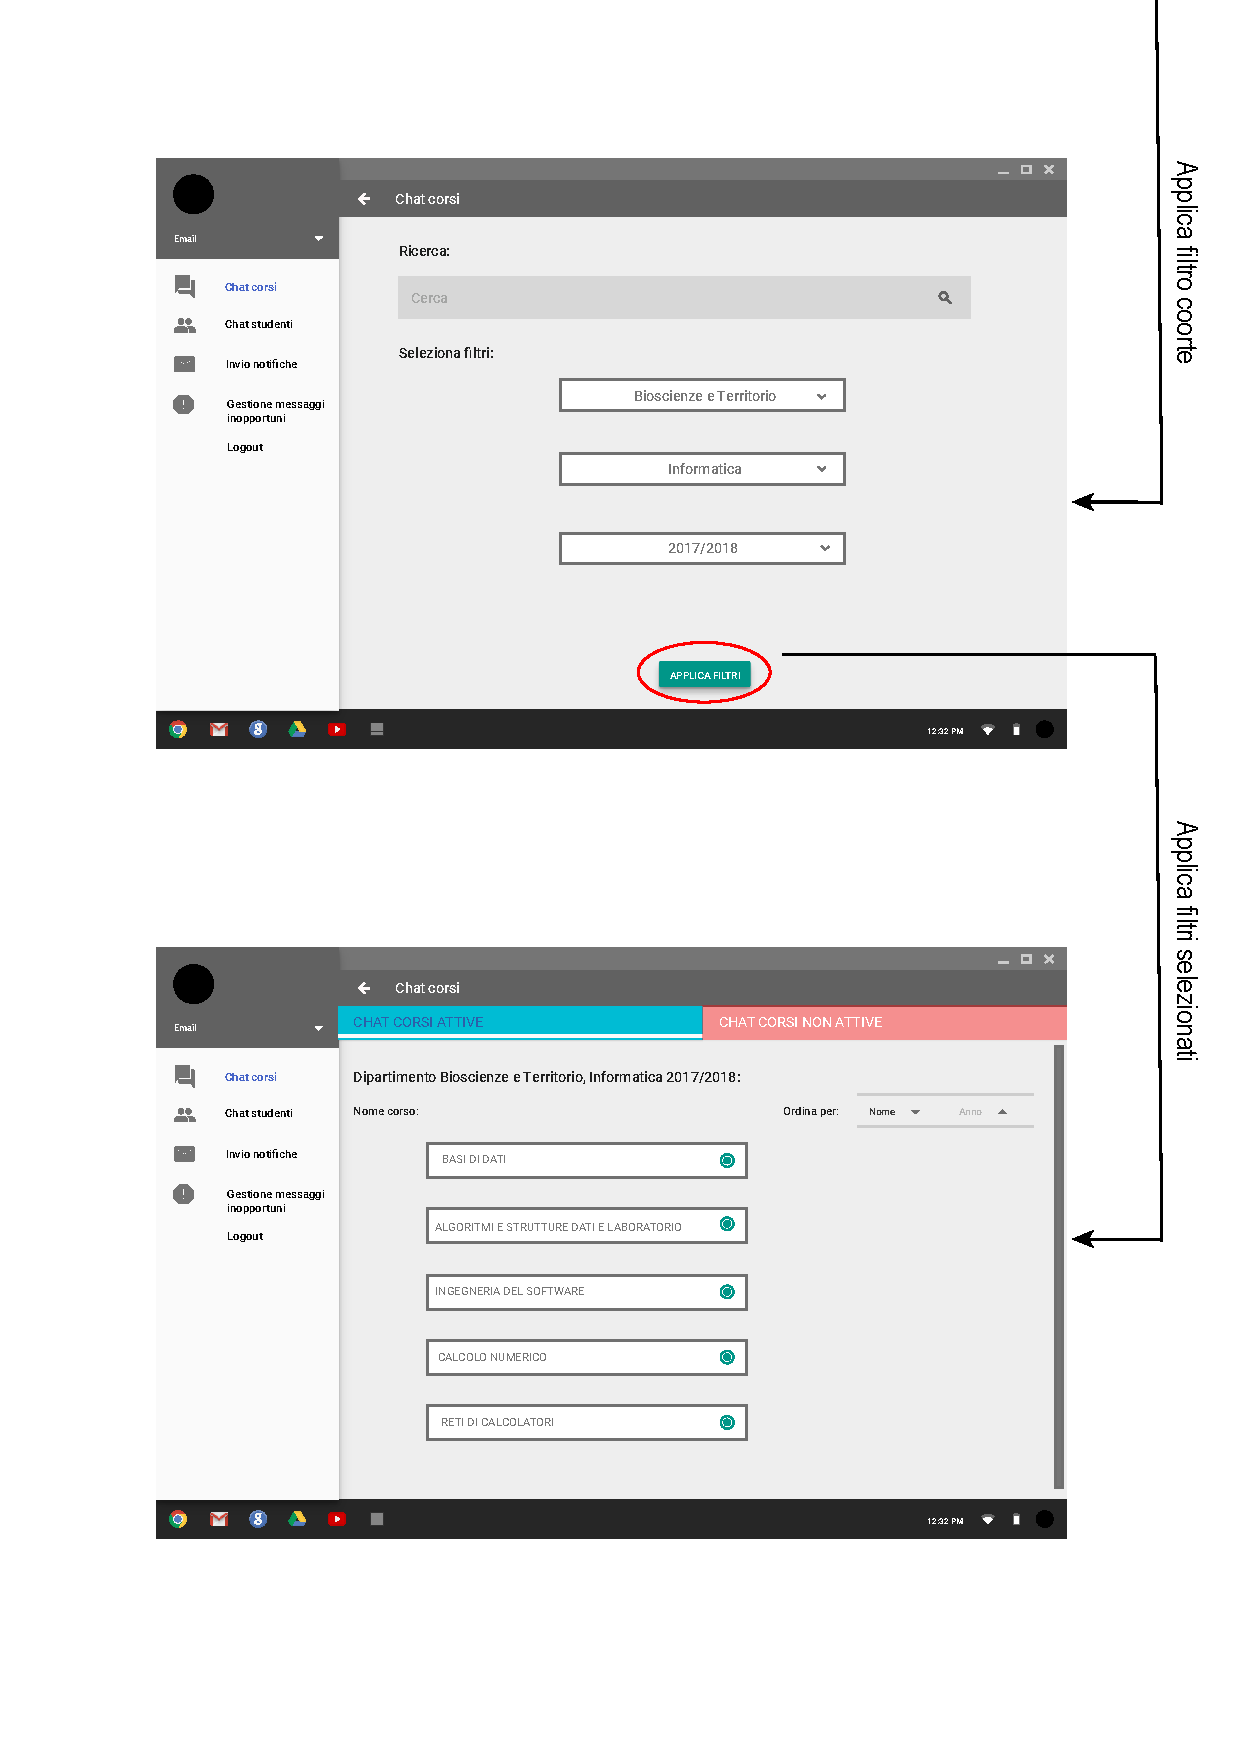
\includegraphics[width=0.9\textwidth]{imgs/gruppo6/activities/act_cup3_filtro_chat_corsi2.pdf}
	\caption{CUP3 - Ricerca chat (filtri chat corsi - pt.2)}
	\label{fig:cup3-2}
\end{figure}

\begin{figure}
	\centering
	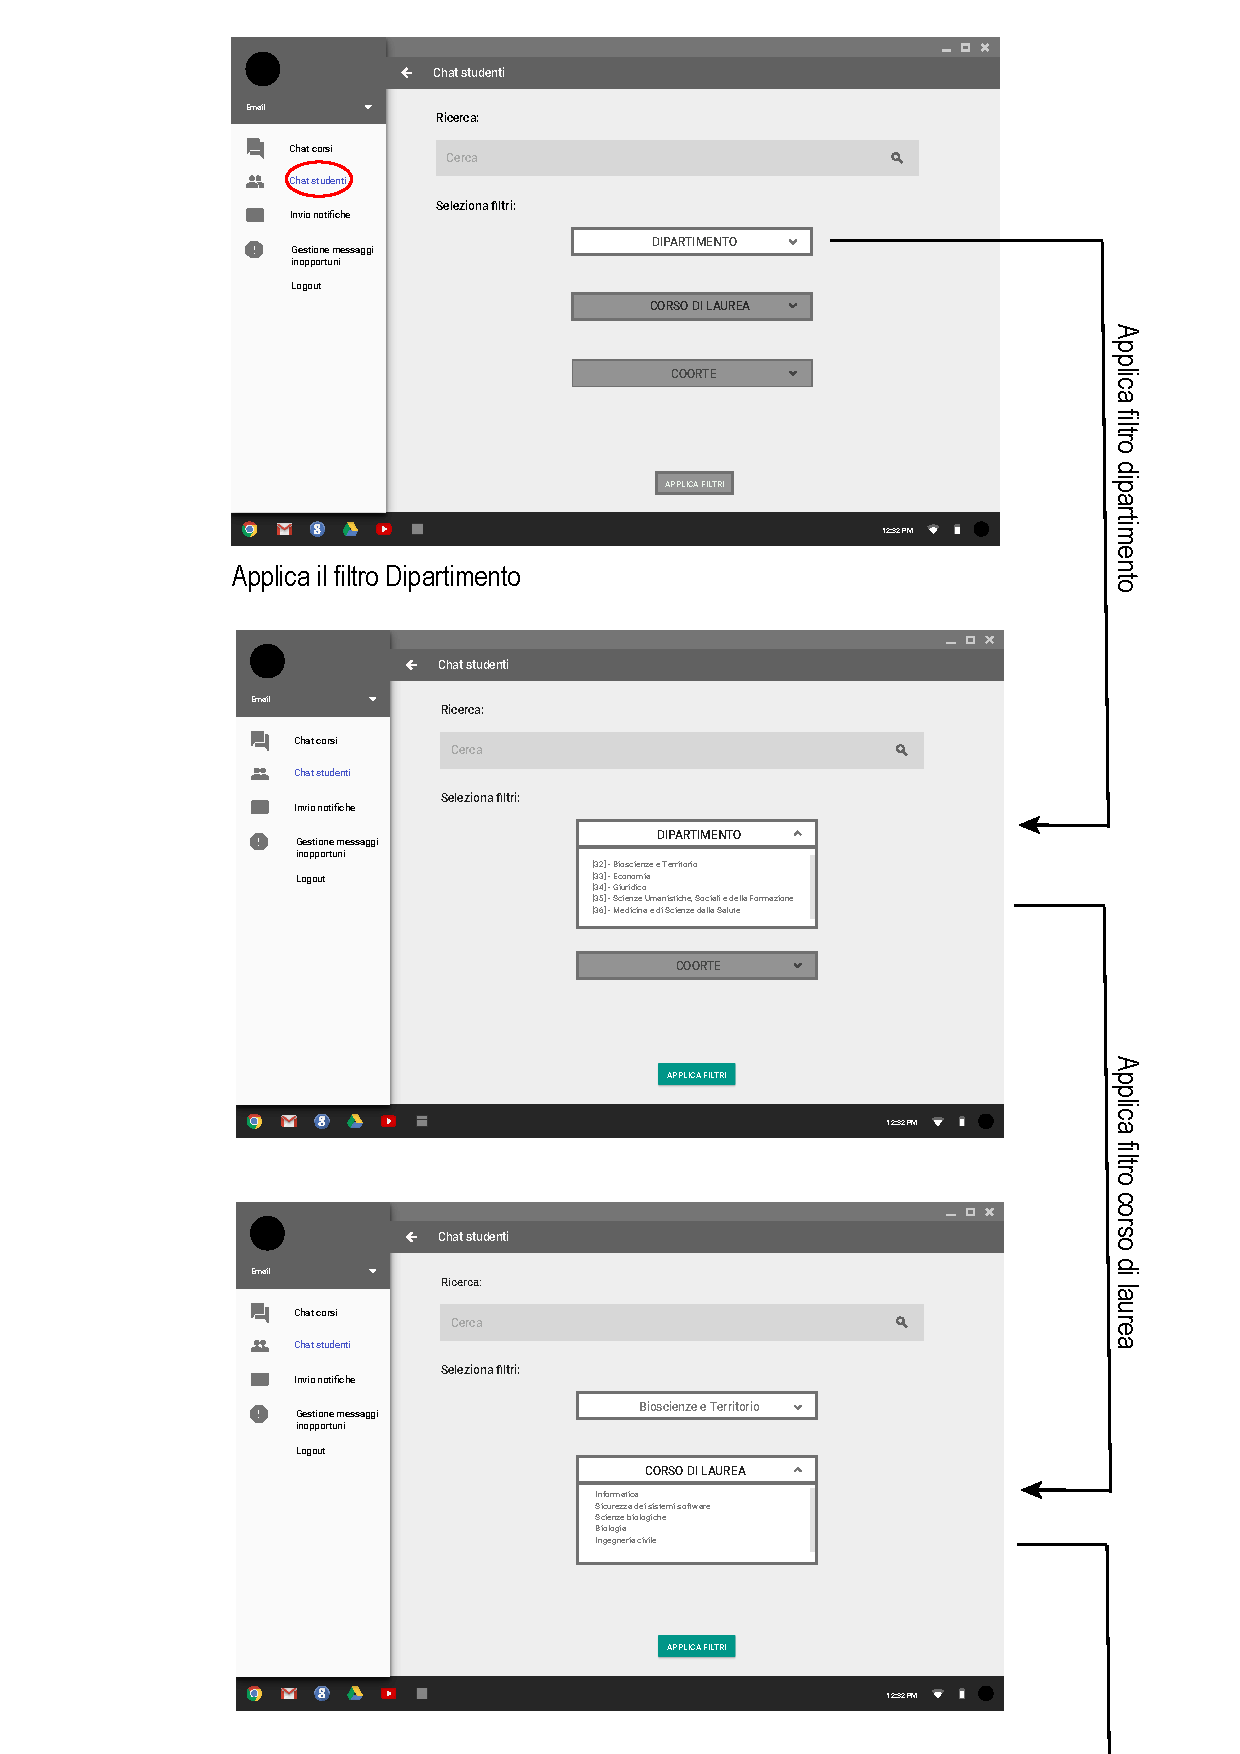
\includegraphics[width=0.9\textwidth]{imgs/gruppo6/activities/act_cup3_filtro_chat_studenti1.pdf}
	\caption{CUP3 - Ricerca chat (filtri chat studenti - pt.1)}
	\label{fig:cup3-3}
\end{figure}

\begin{figure}
	\centering
	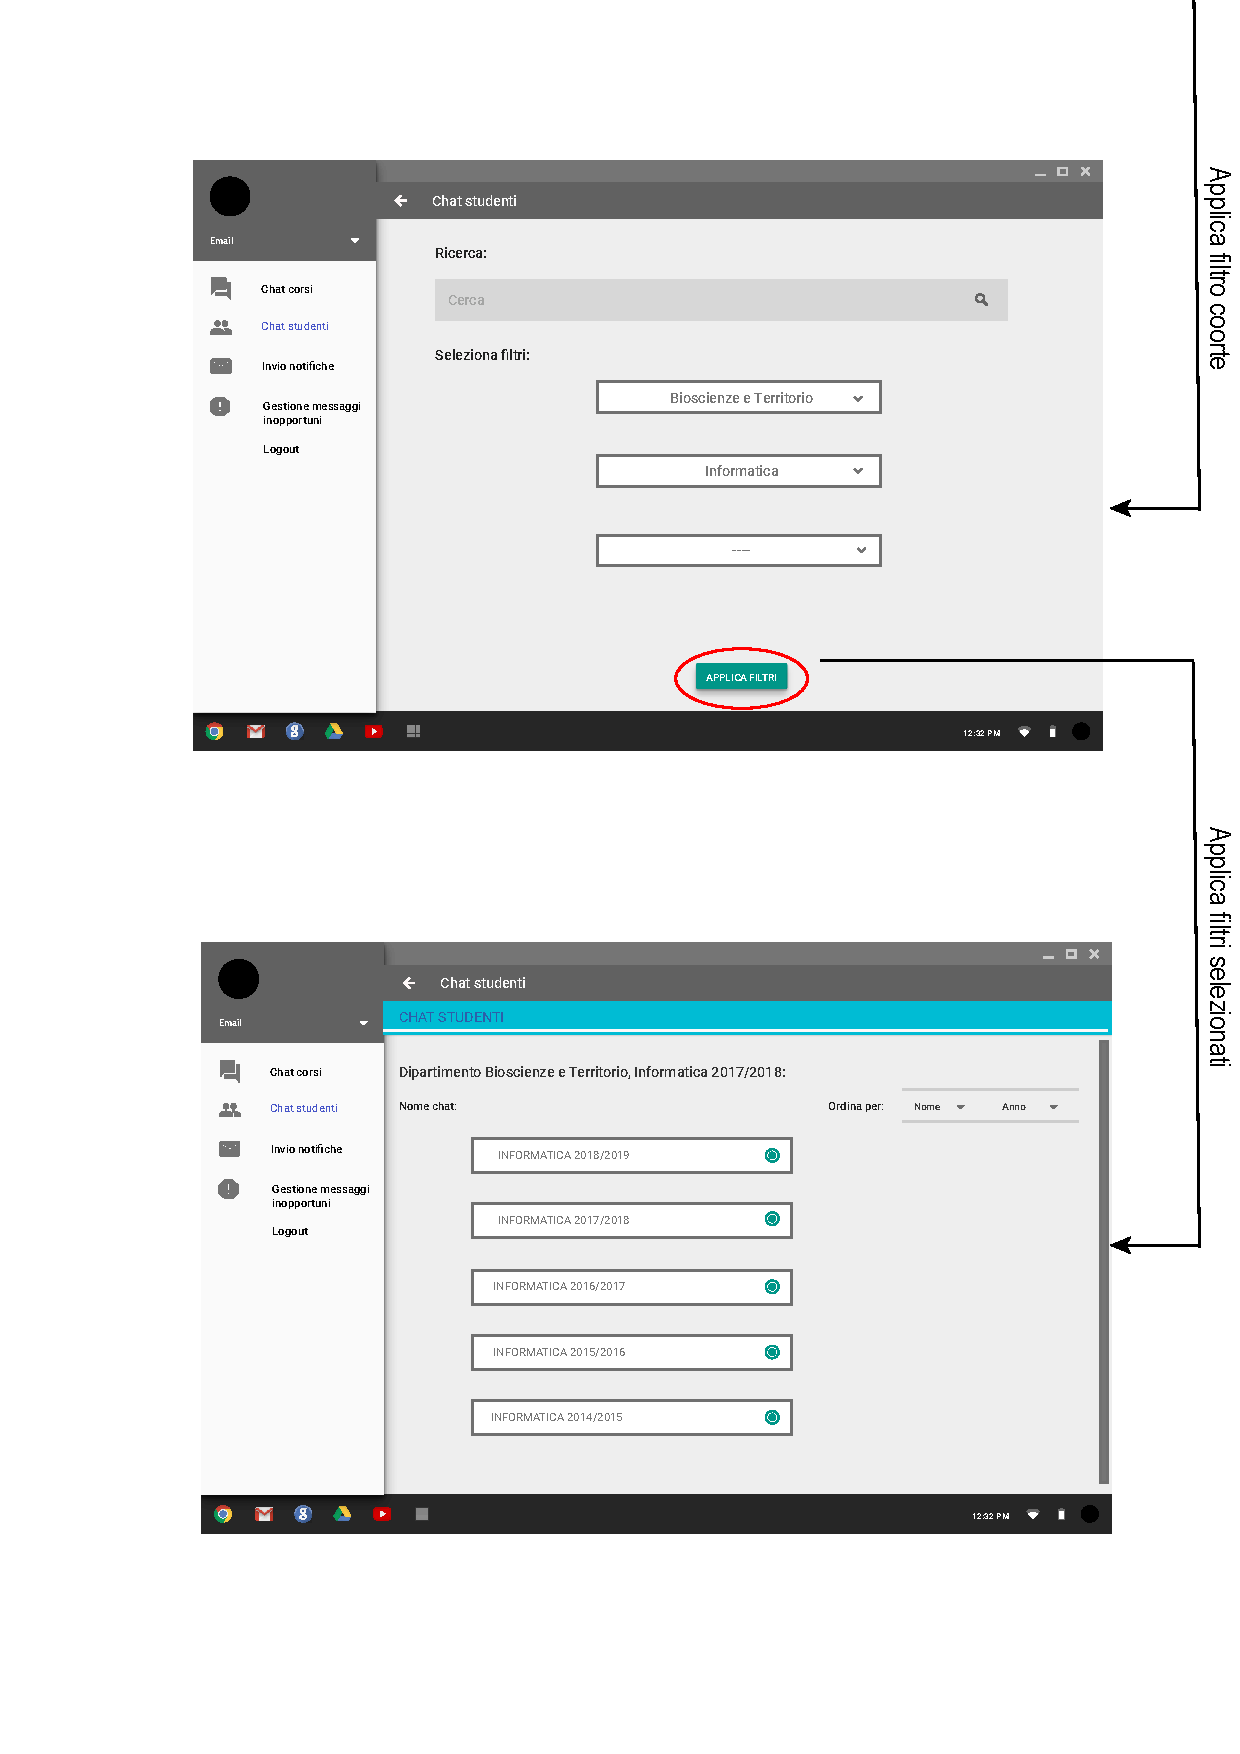
\includegraphics[width=0.9\textwidth]{imgs/gruppo6/activities/act_cup3_filtro_chat_studenti2.pdf}
	\caption{CUP3 - Ricerca chat (filtri chat studenti - pt.2)}
	\label{fig:cup3-4}
\end{figure}

\begin{figure}
	\centering
	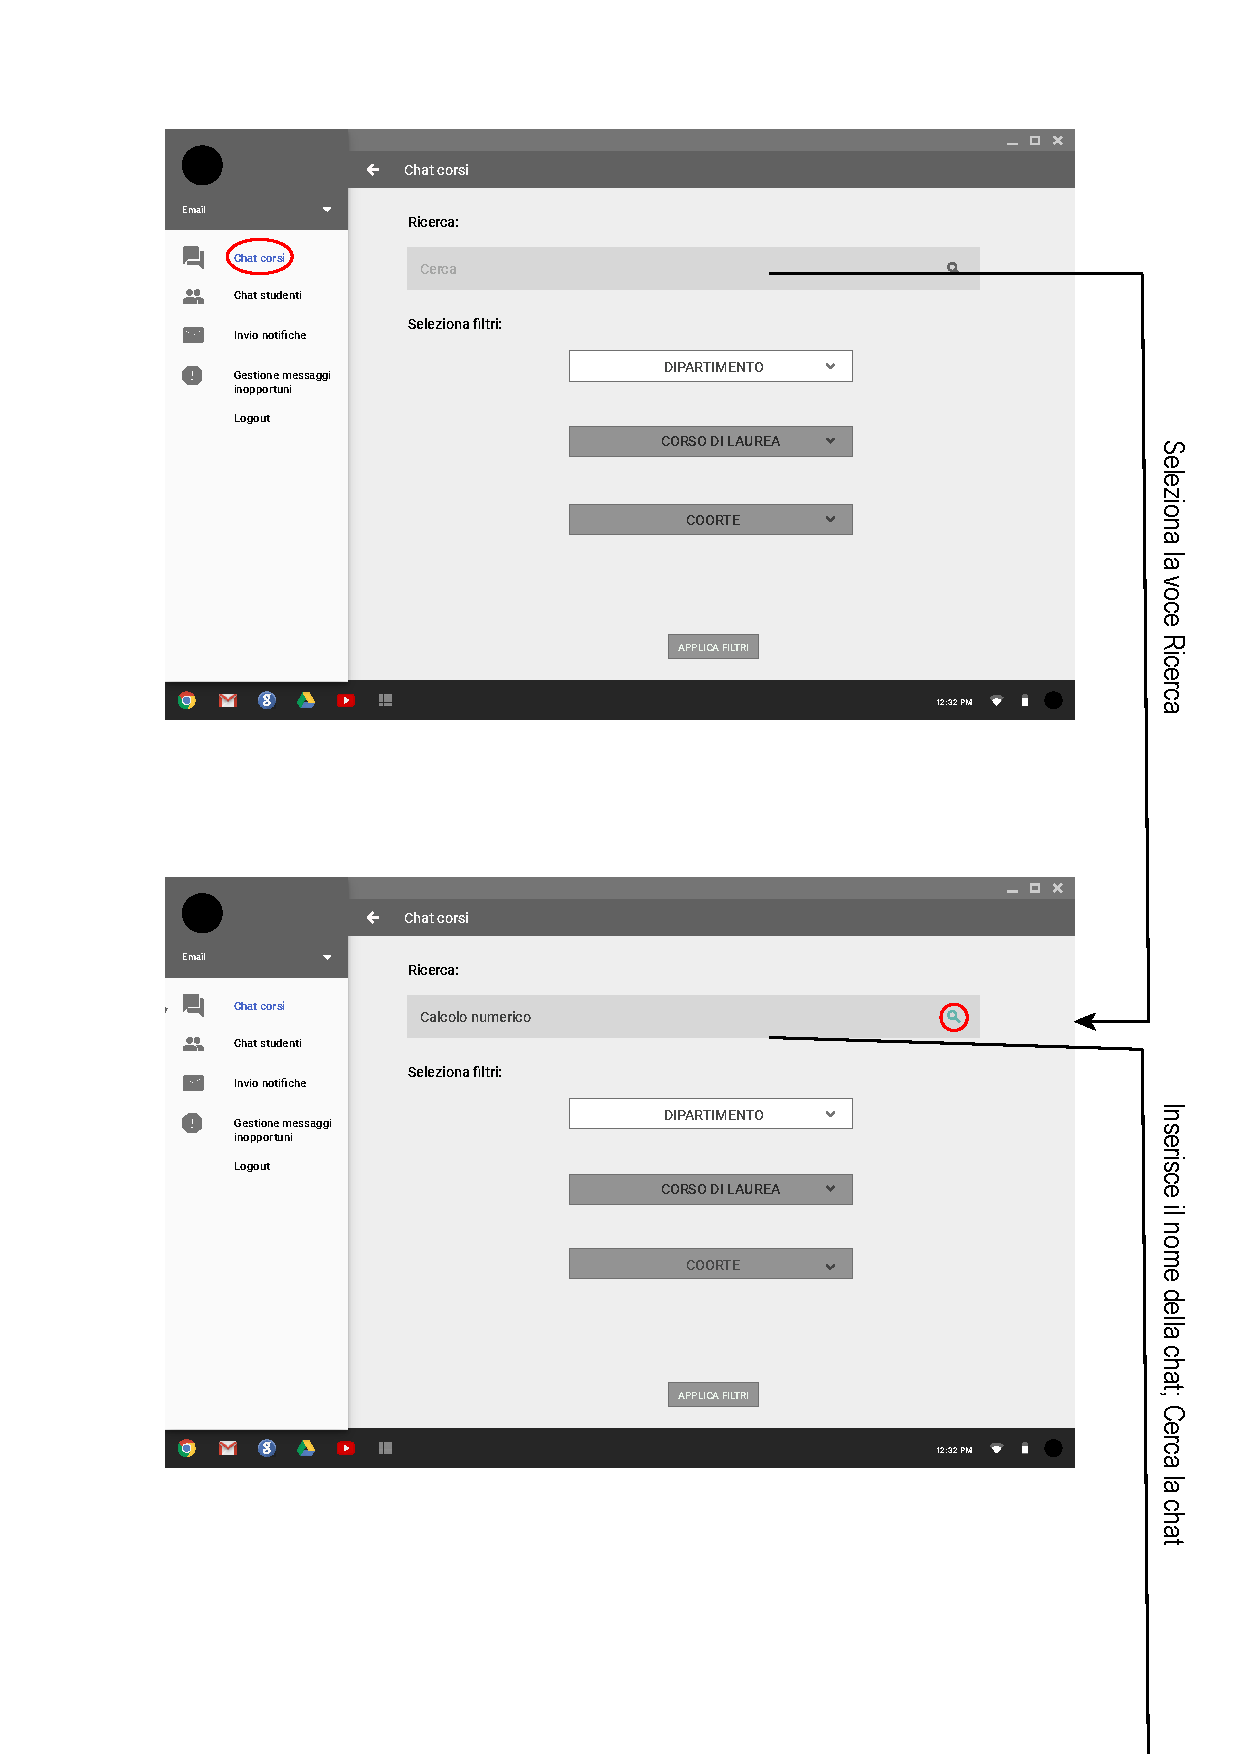
\includegraphics[width=0.9\textwidth]{imgs/gruppo6/activities/act_cup3_ricerca_chat_corsi1.pdf}
	\caption{CUP3 - Ricerca chat (cerca corsi - pt.1)}
	\label{fig:cup3-5}
\end{figure}

\begin{figure}
	\centering
	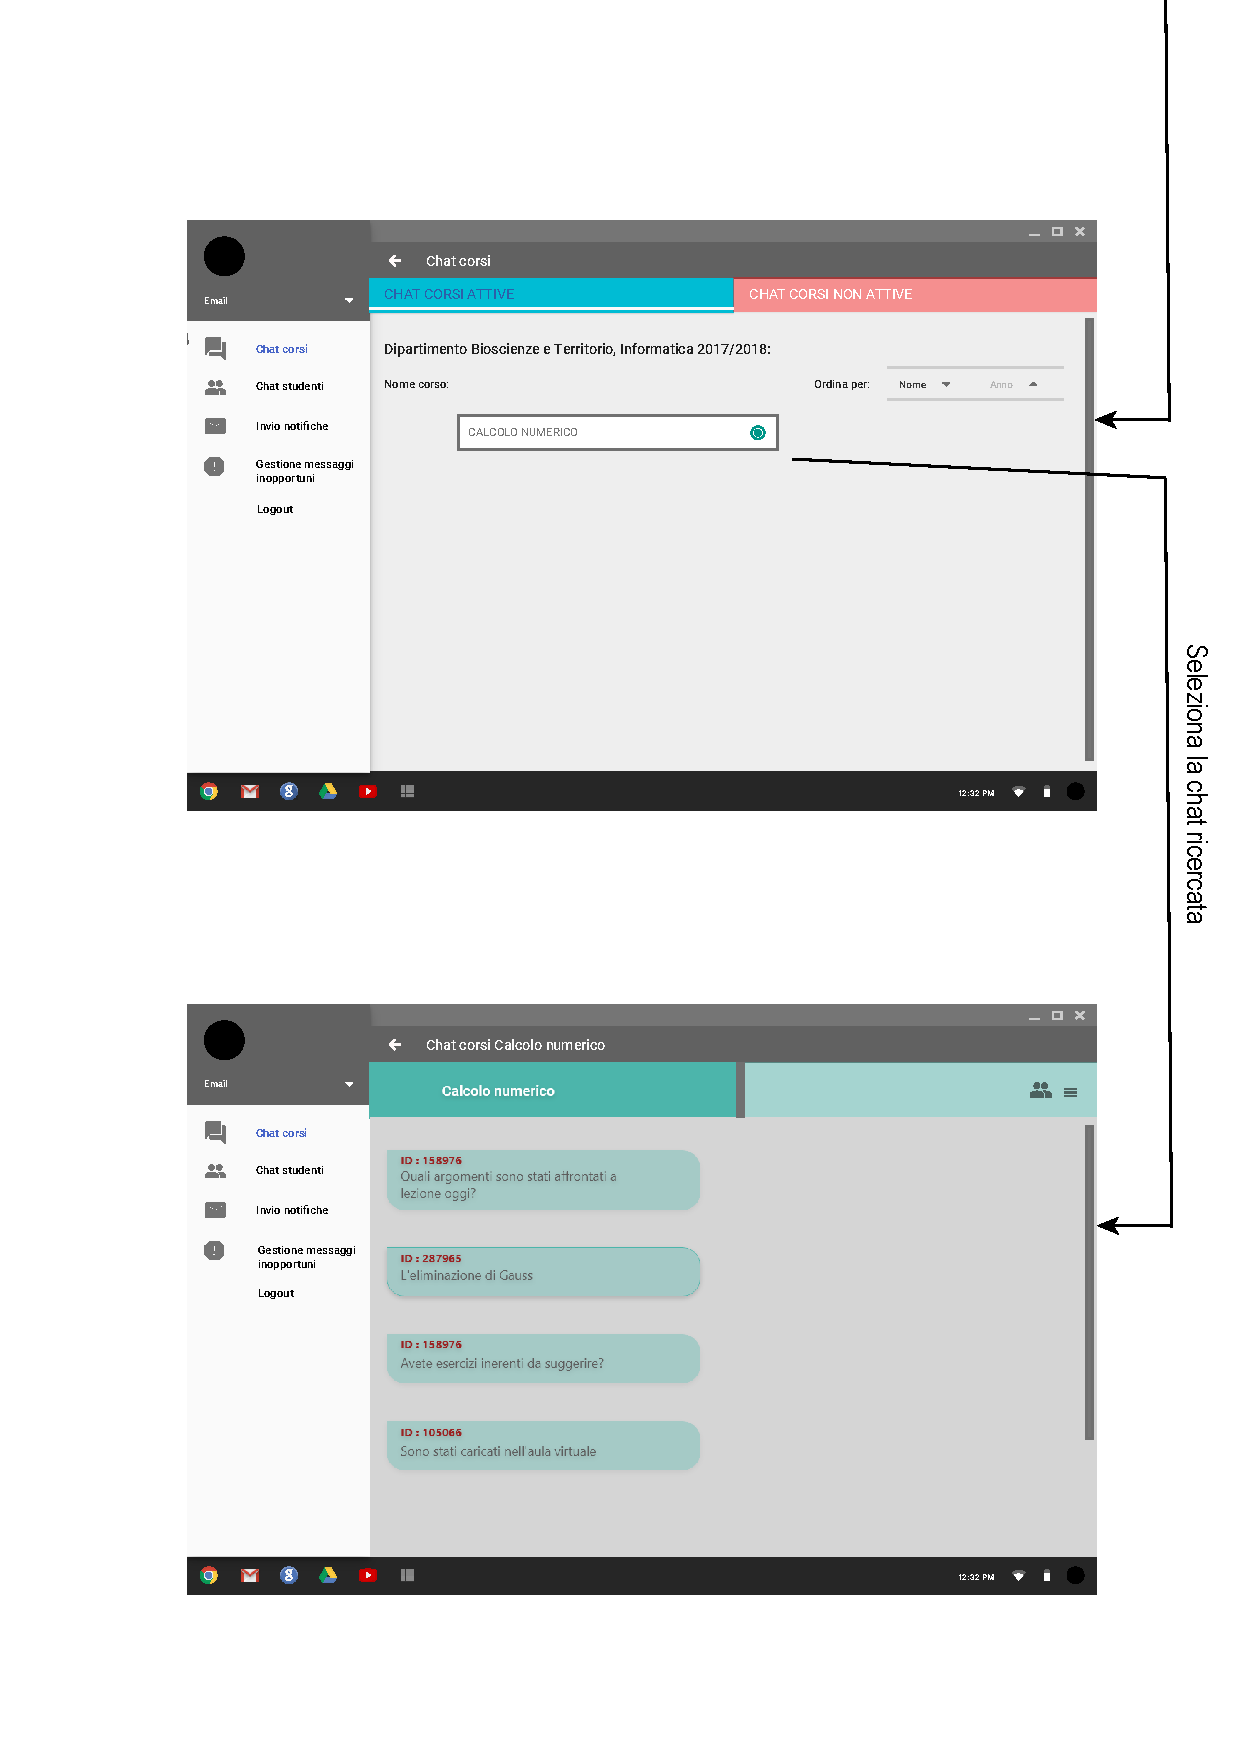
\includegraphics[width=0.9\textwidth]{imgs/gruppo6/activities/act_cup3_ricerca_chat_corsi2.pdf}
	\caption{CUP3 - Ricerca chat (cerca corsi - pt.2)}
	\label{fig:cup3-6}
\end{figure}

\begin{figure}
	\centering
	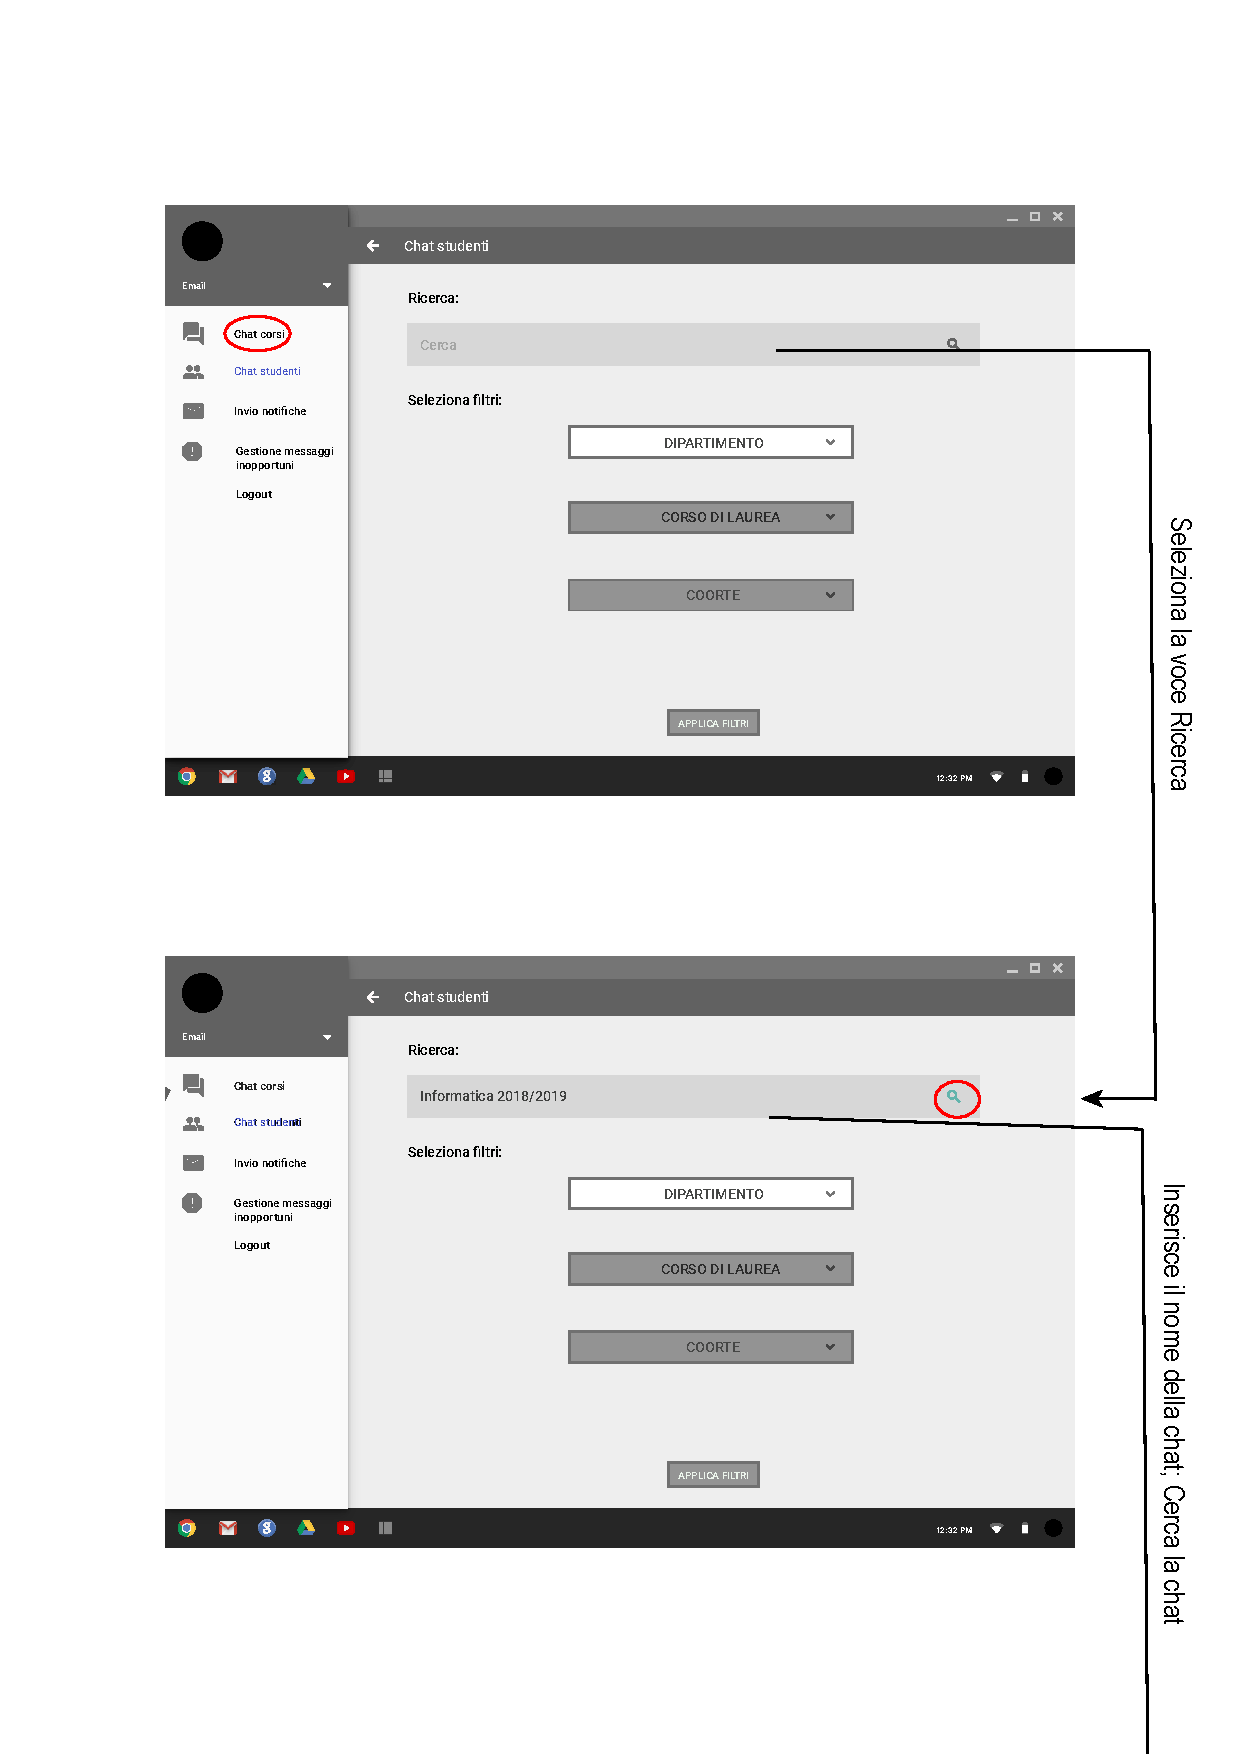
\includegraphics[width=0.9\textwidth]{imgs/gruppo6/activities/act_cup3_ricerca_chat_studenti.pdf}
	\caption{CUP3 - Ricerca chat (cerca studenti - pt.1)}
	\label{fig:cup3-7}
\end{figure}

\begin{figure}
	\centering
	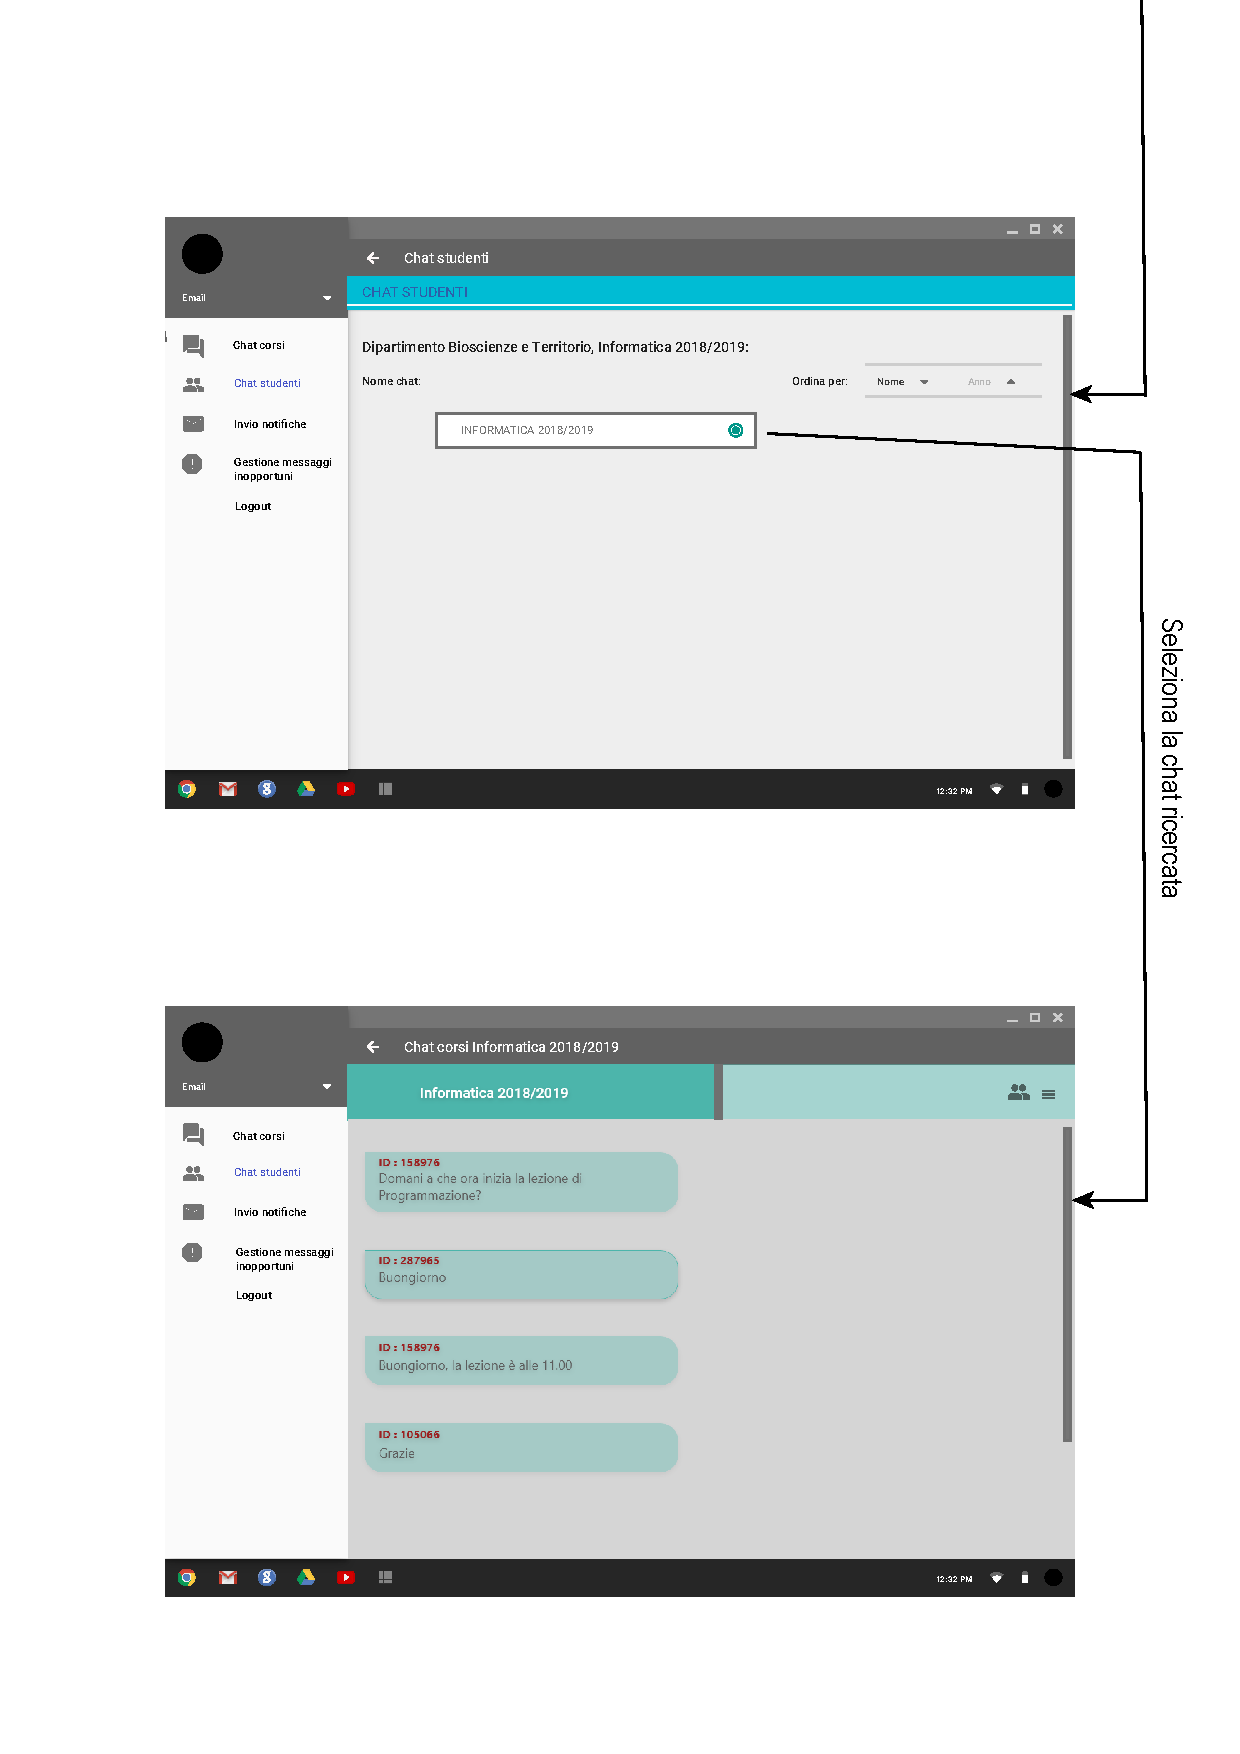
\includegraphics[width=0.9\textwidth]{imgs/gruppo6/activities/act_cup3_ricerca_chat_studenti2.pdf}
	\caption{CUP3 - Ricerca chat (cerca studenti - pt.2)}
	\label{fig:cup3-8}
\end{figure}

\begin{figure}
	\centering
	\includegraphics[width=0.9\textwidth]{imgs/gruppo6/activities/act_cup4_visualizza_lista_chat_corsi1.pdf}
	\caption{CUP4 - Visualizza lista chat (corsi - pt.1)}
	\label{fig:cup4}
\end{figure}

\begin{figure}
	\centering
	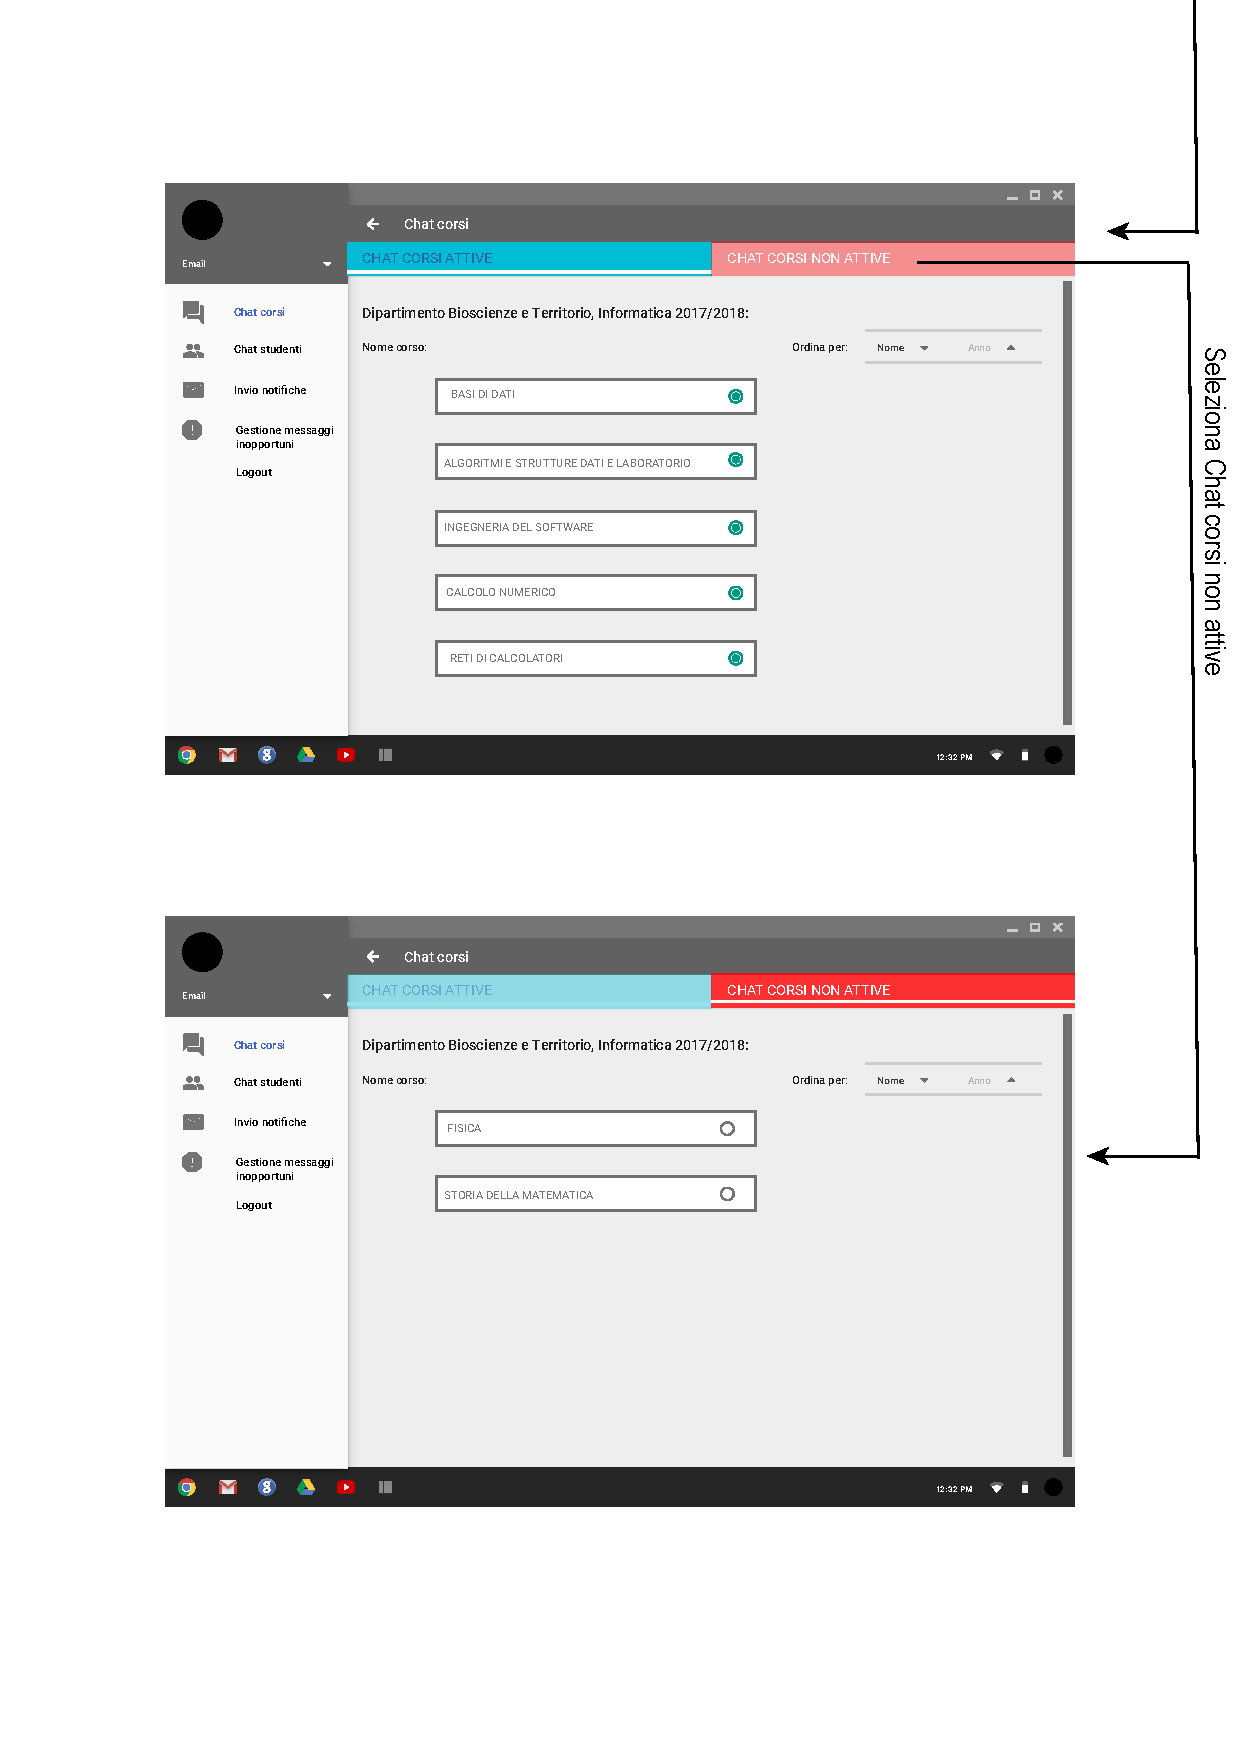
\includegraphics[width=0.9\textwidth]{imgs/gruppo6/activities/act_cup4_visualizza_lista_chat_corsi2.pdf}
	\caption{CUP4 - Visualizza lista chat (corsi - pt.2)}
	\label{fig:cup4-2}
\end{figure}

\begin{figure}
	\centering
	\includegraphics[width=0.9\textwidth]{imgs/gruppo6/activities/act_cup4_visualizza_lista_chat_studenti.pdf}
	\caption{CUP4 - Visualizza lista chat (studenti)}
	\label{fig:cup4-3}
\end{figure}

\begin{figure}
	\centering
	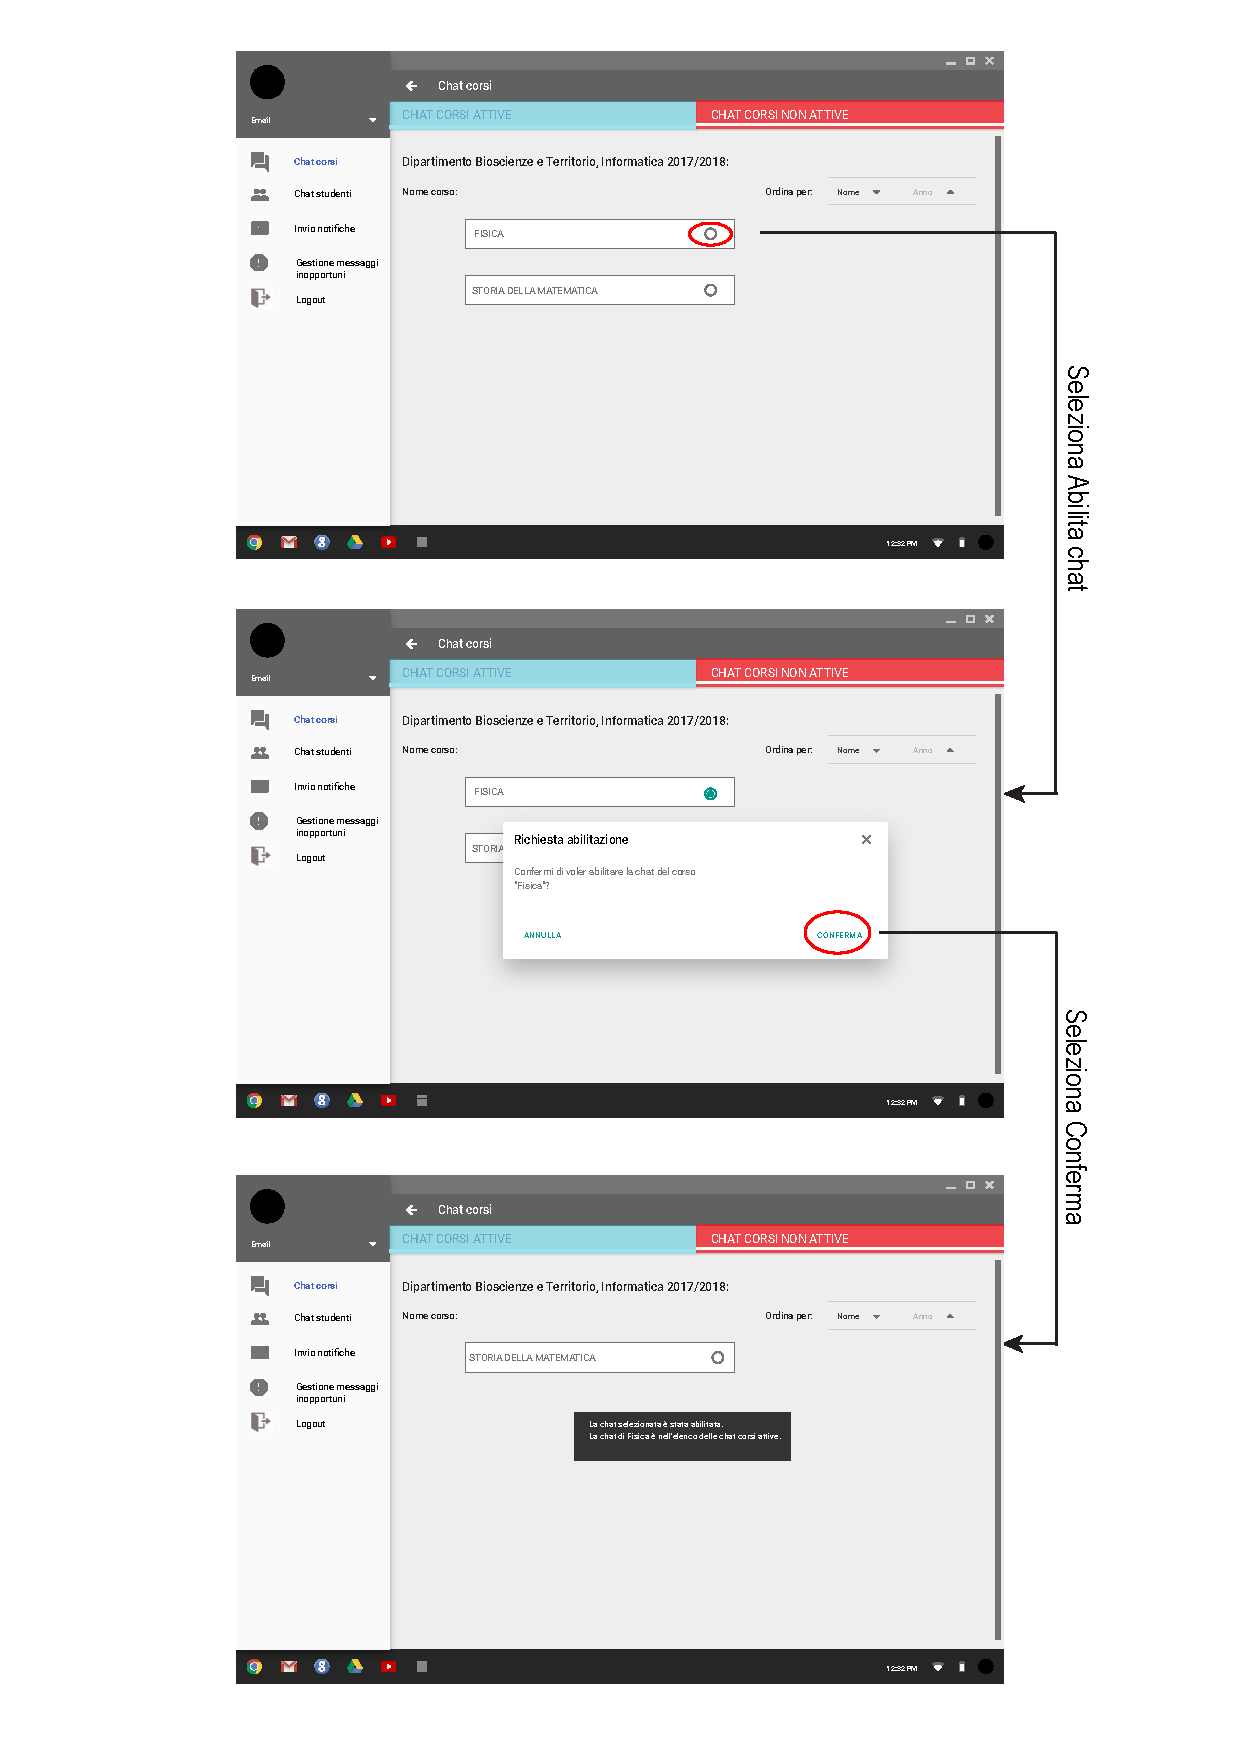
\includegraphics[width=0.9\textwidth]{imgs/gruppo6/activities/act_cup5_abilita_chat.pdf}
	\caption{CUP5 - Abilita chat}
	\label{fig:cup5}
\end{figure}

\begin{figure}
	\centering
	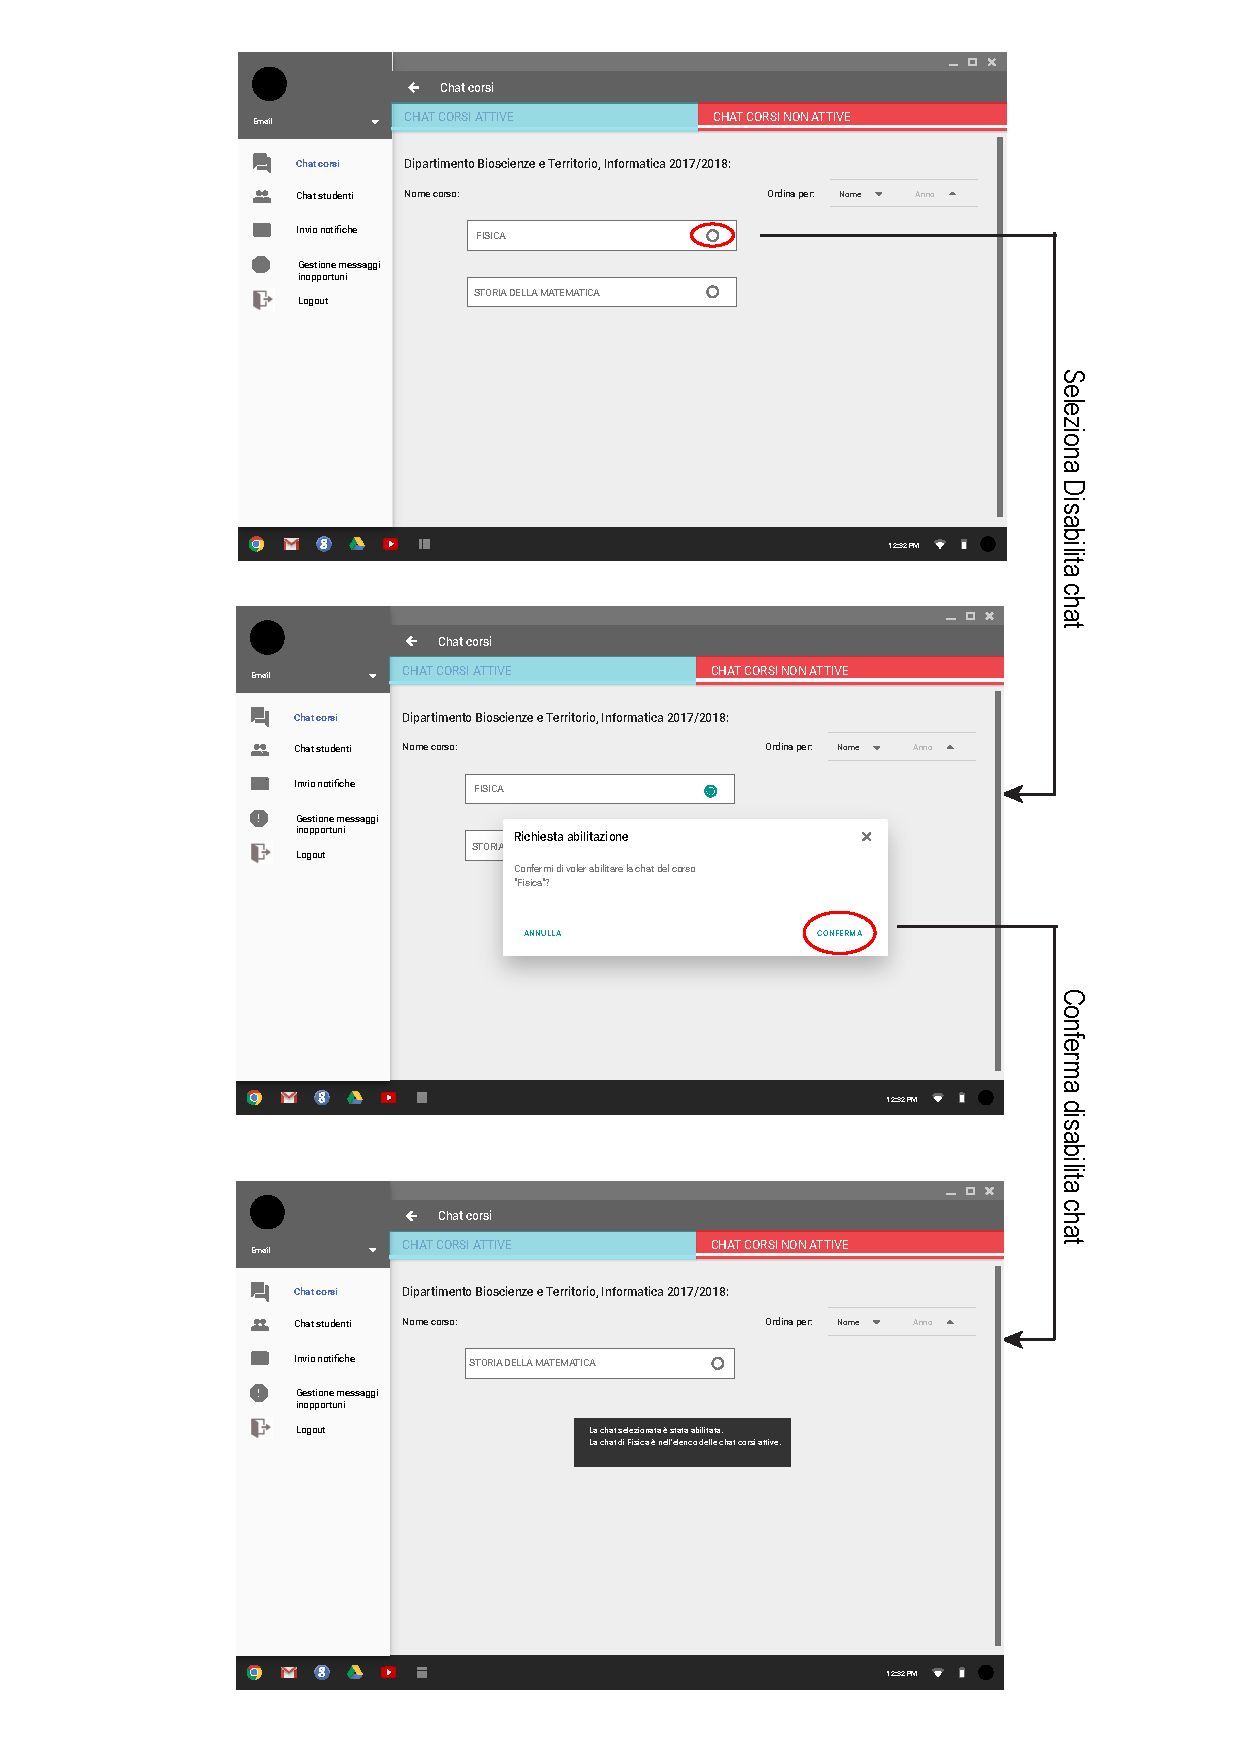
\includegraphics[width=0.9\textwidth]{imgs/gruppo6/activities/act_cup6_disabilita_chat.pdf}
	\caption{CUP6 - Disabilita chat}
	\label{fig:cup6}
\end{figure}

\begin{figure}
	\centering
	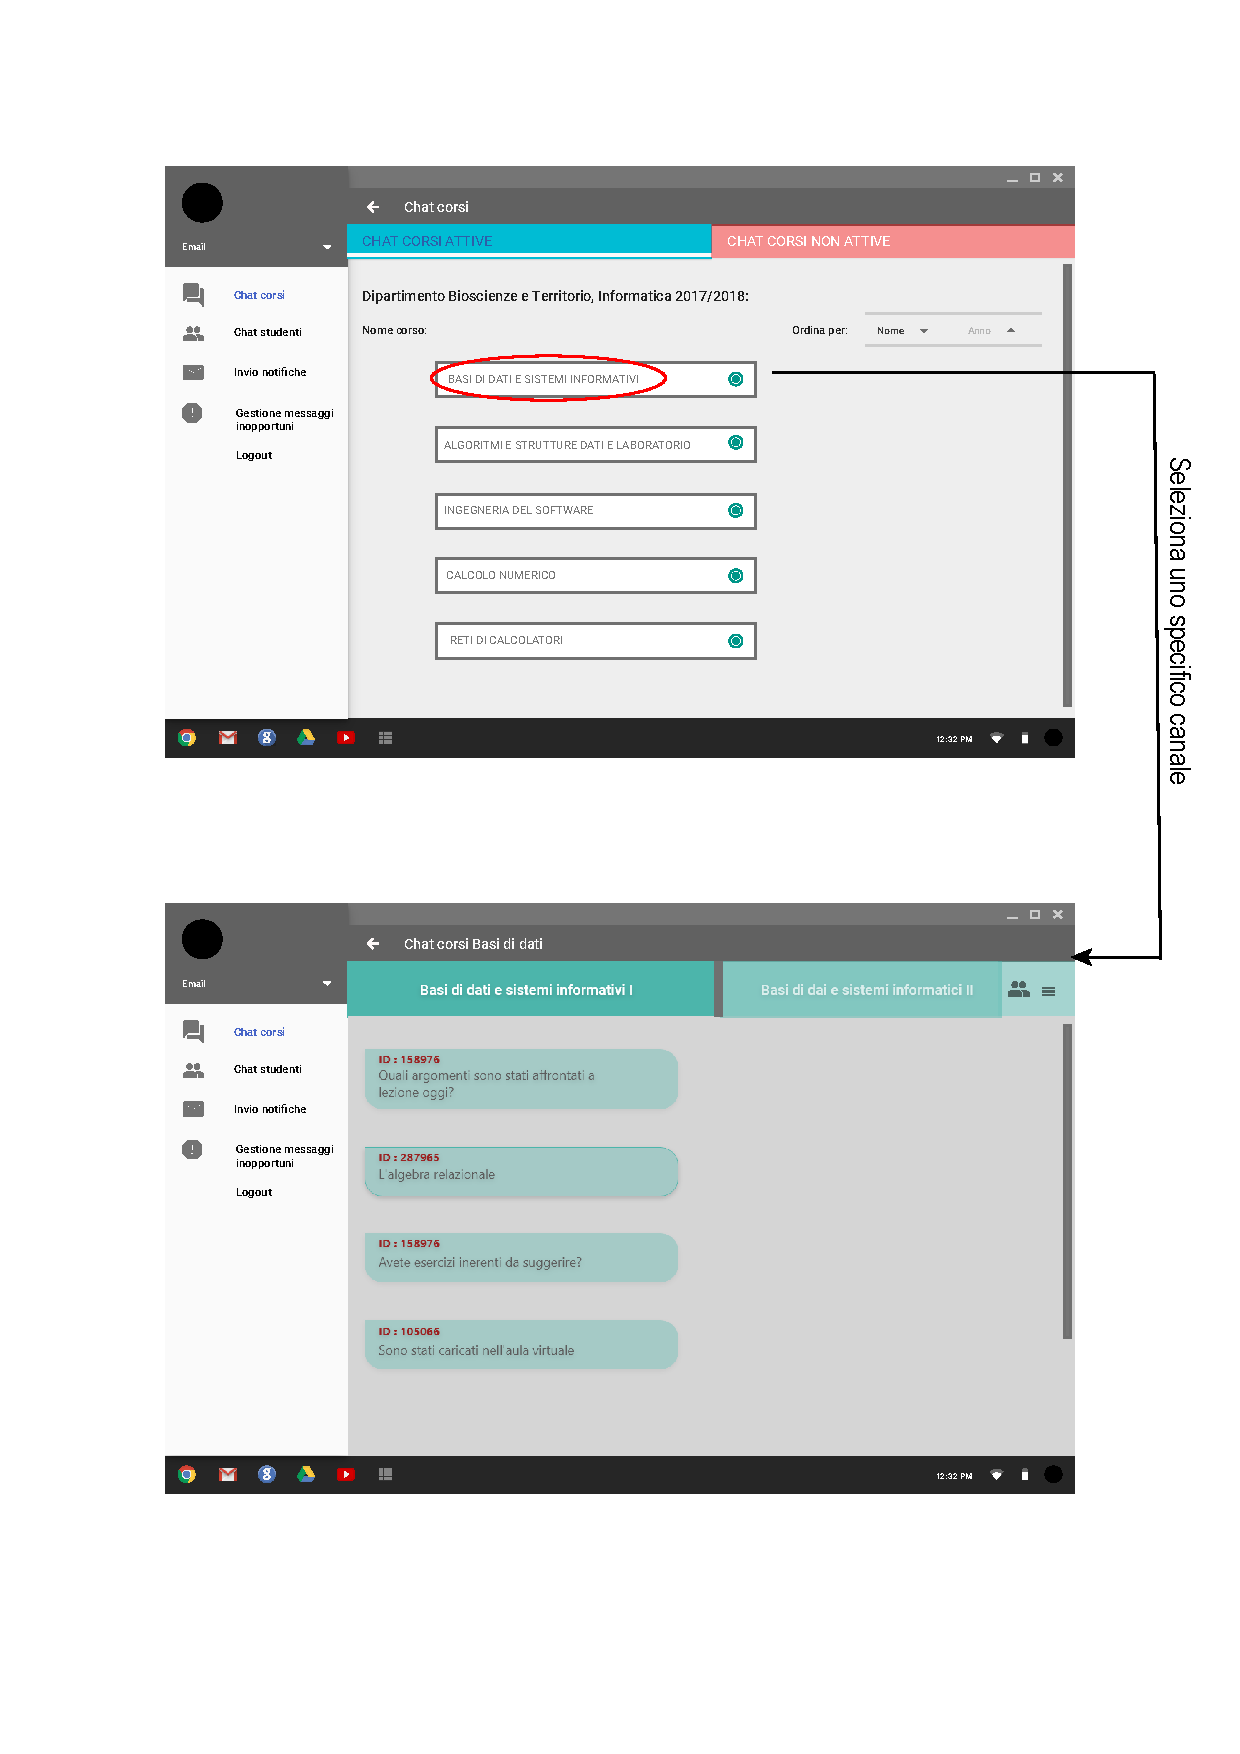
\includegraphics[width=0.9\textwidth]{imgs/gruppo6/activities/act_cup7_visualizza_canale.pdf}
	\caption{CUP7 - Visualizza canale}
	\label{fig:cup7}
\end{figure}

\begin{figure}
	\centering
	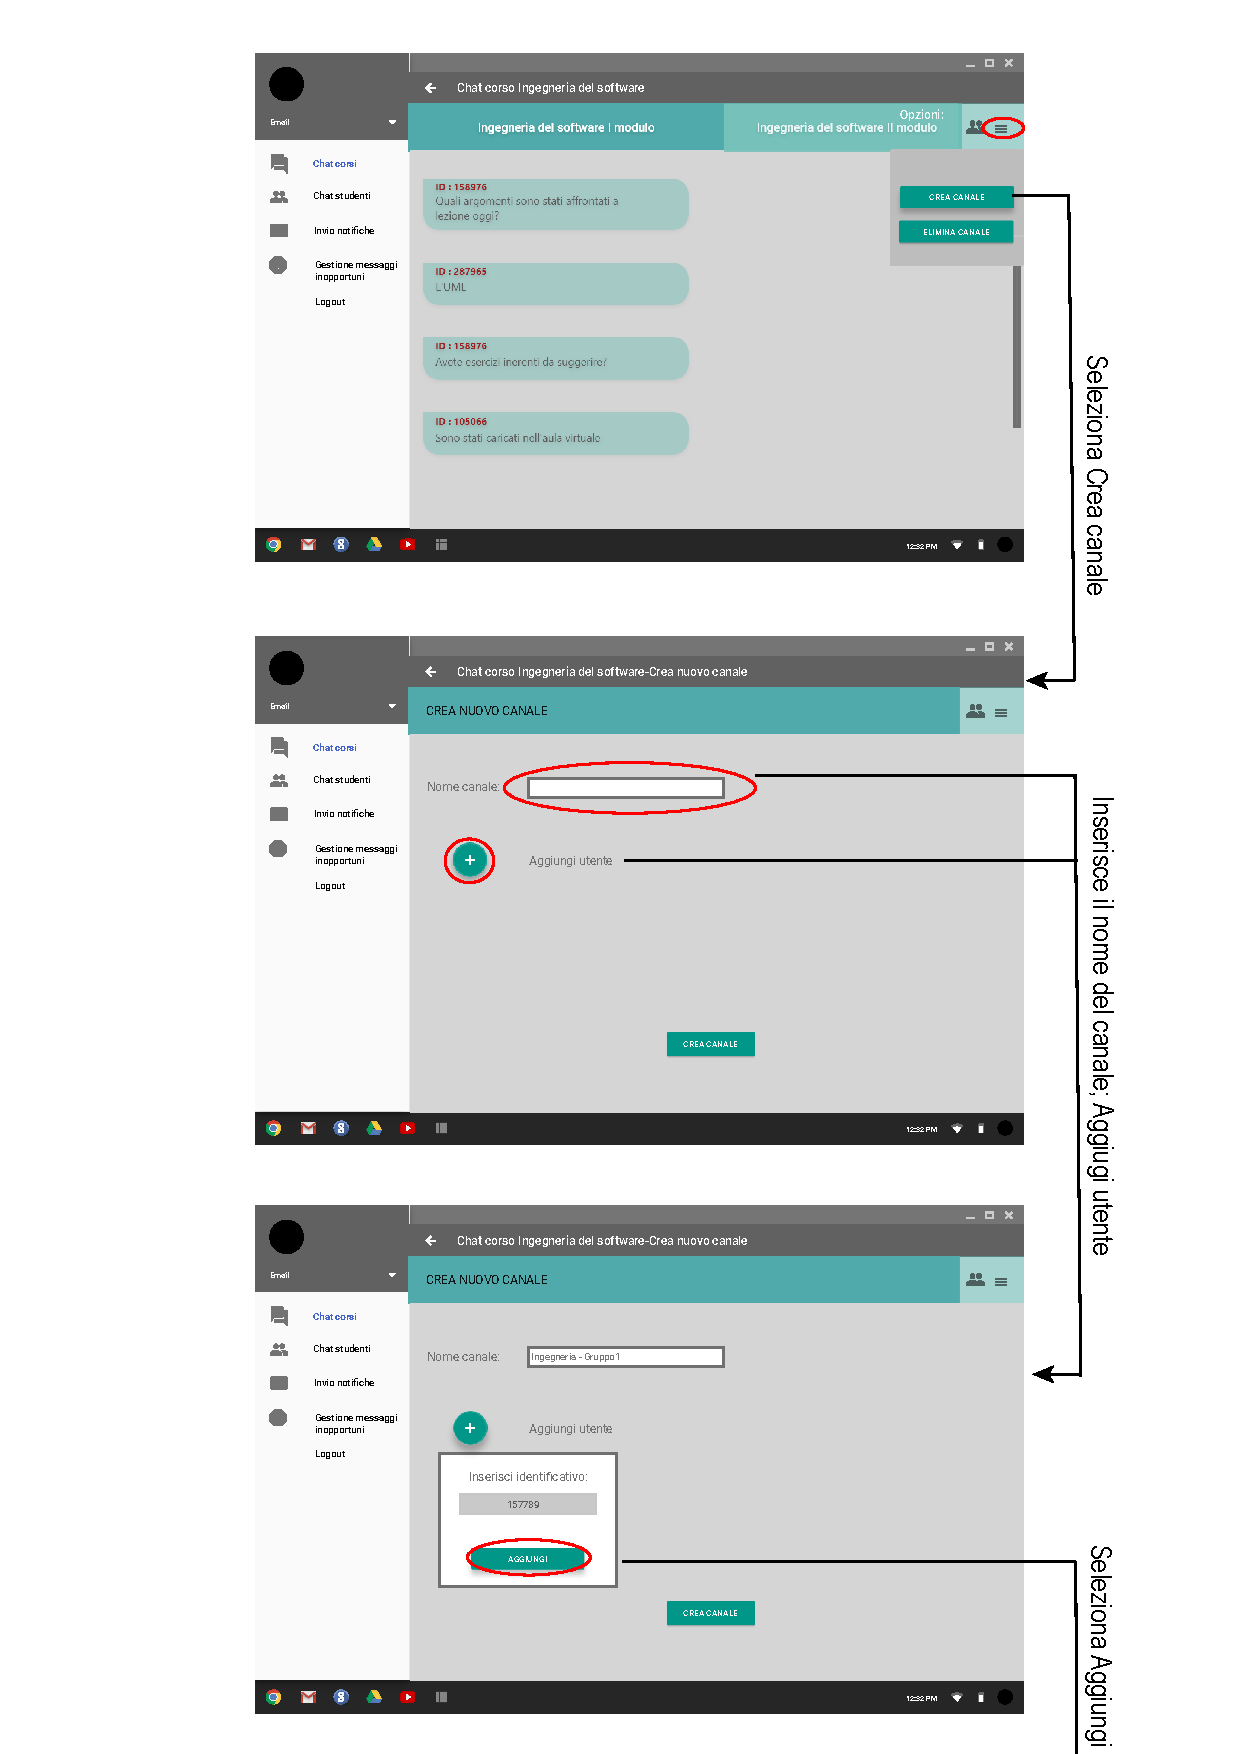
\includegraphics[width=0.9\textwidth]{imgs/gruppo6/activities/act_cup8_aggiungi_canale1.pdf}
	\caption{CUP8 - Aggiungi canale (pt.1)}
	\label{fig:cup8}
\end{figure}

\begin{figure}
	\centering
	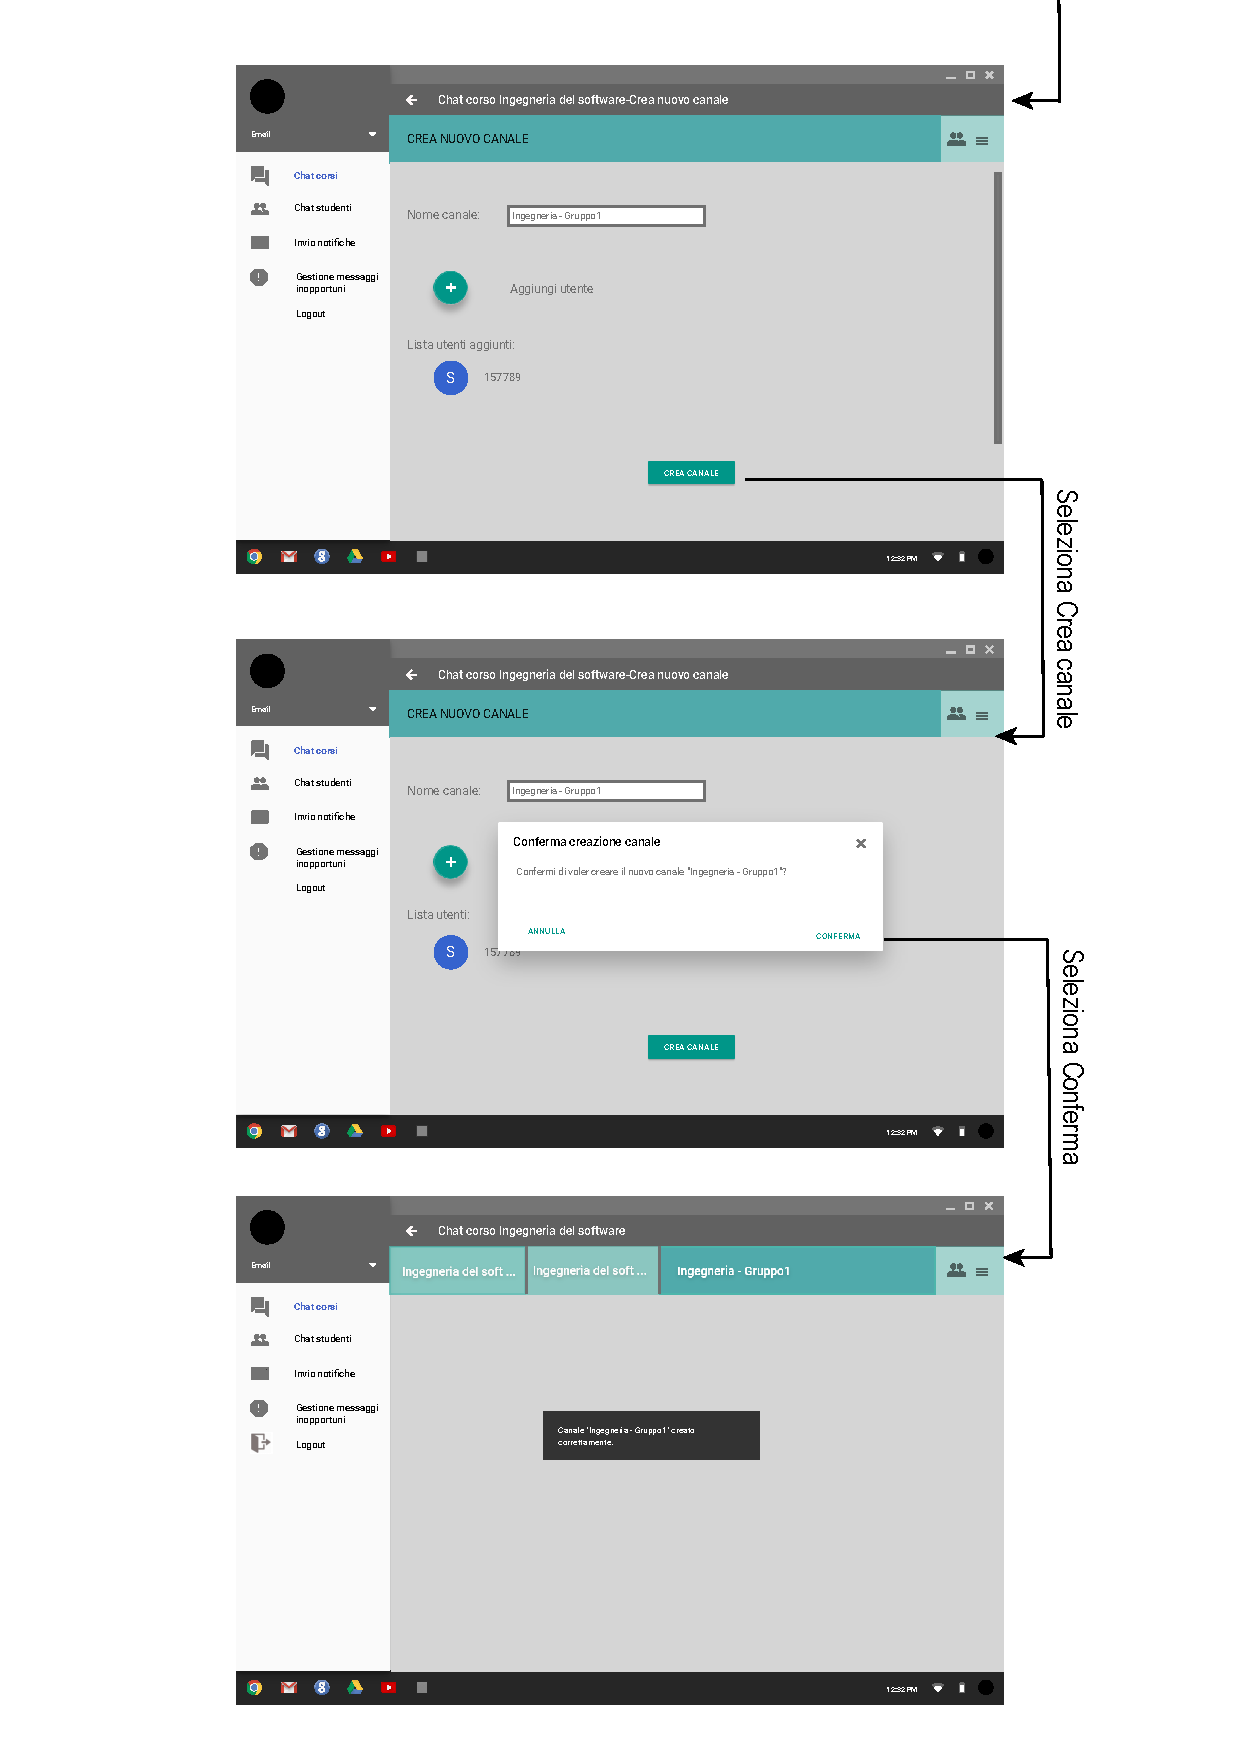
\includegraphics[width=0.9\textwidth]{imgs/gruppo6/activities/act_cup8_aggiungi_canale2.pdf}
	\caption{CUP8 - Aggiungi canale (pt.2)}
	\label{fig:cup8-2}
\end{figure}

\begin{figure}
	\centering
	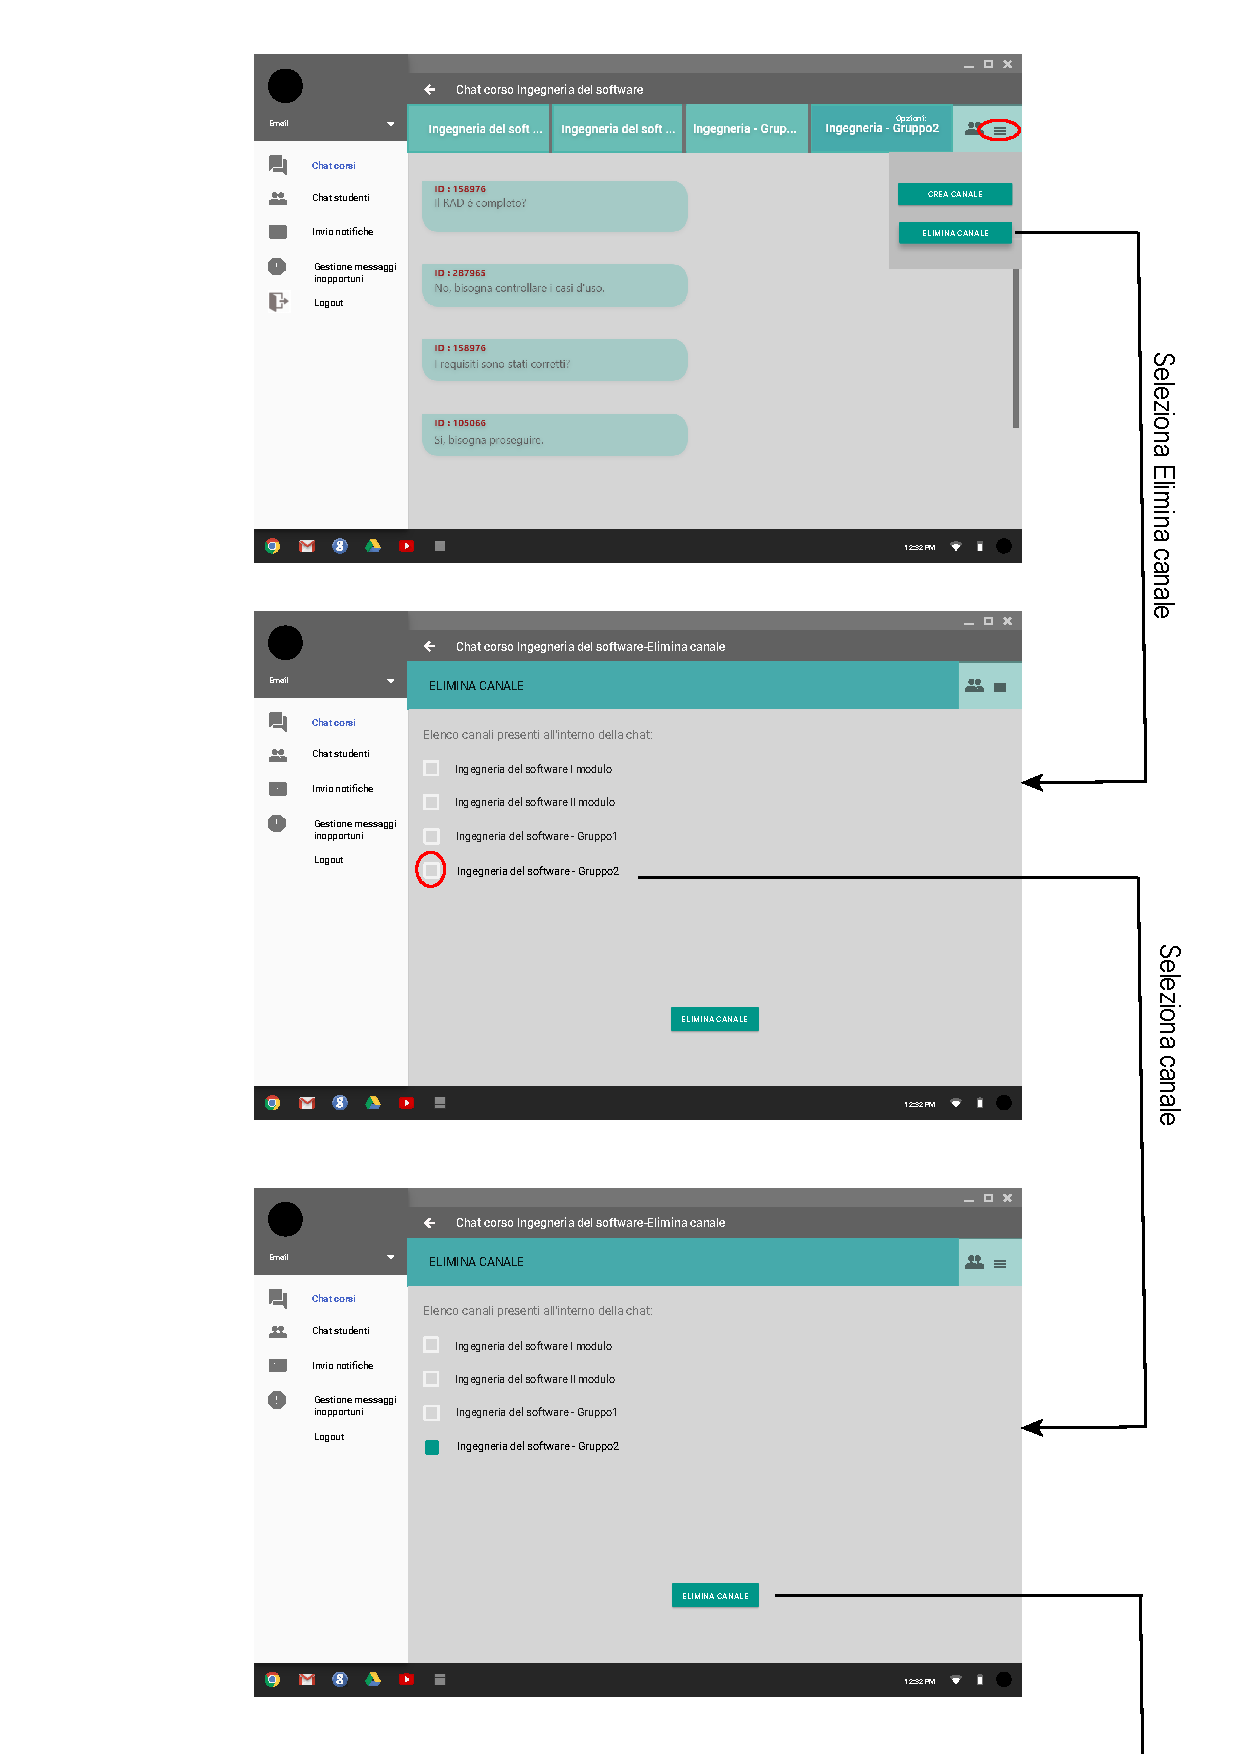
\includegraphics[width=0.9\textwidth]{imgs/gruppo6/activities/act_cup9_cancella_canale1.pdf}
	\caption{CUP9 - Cancella canale (pt.1)}
	\label{fig:cup9}
\end{figure}

\begin{figure}
	\centering
	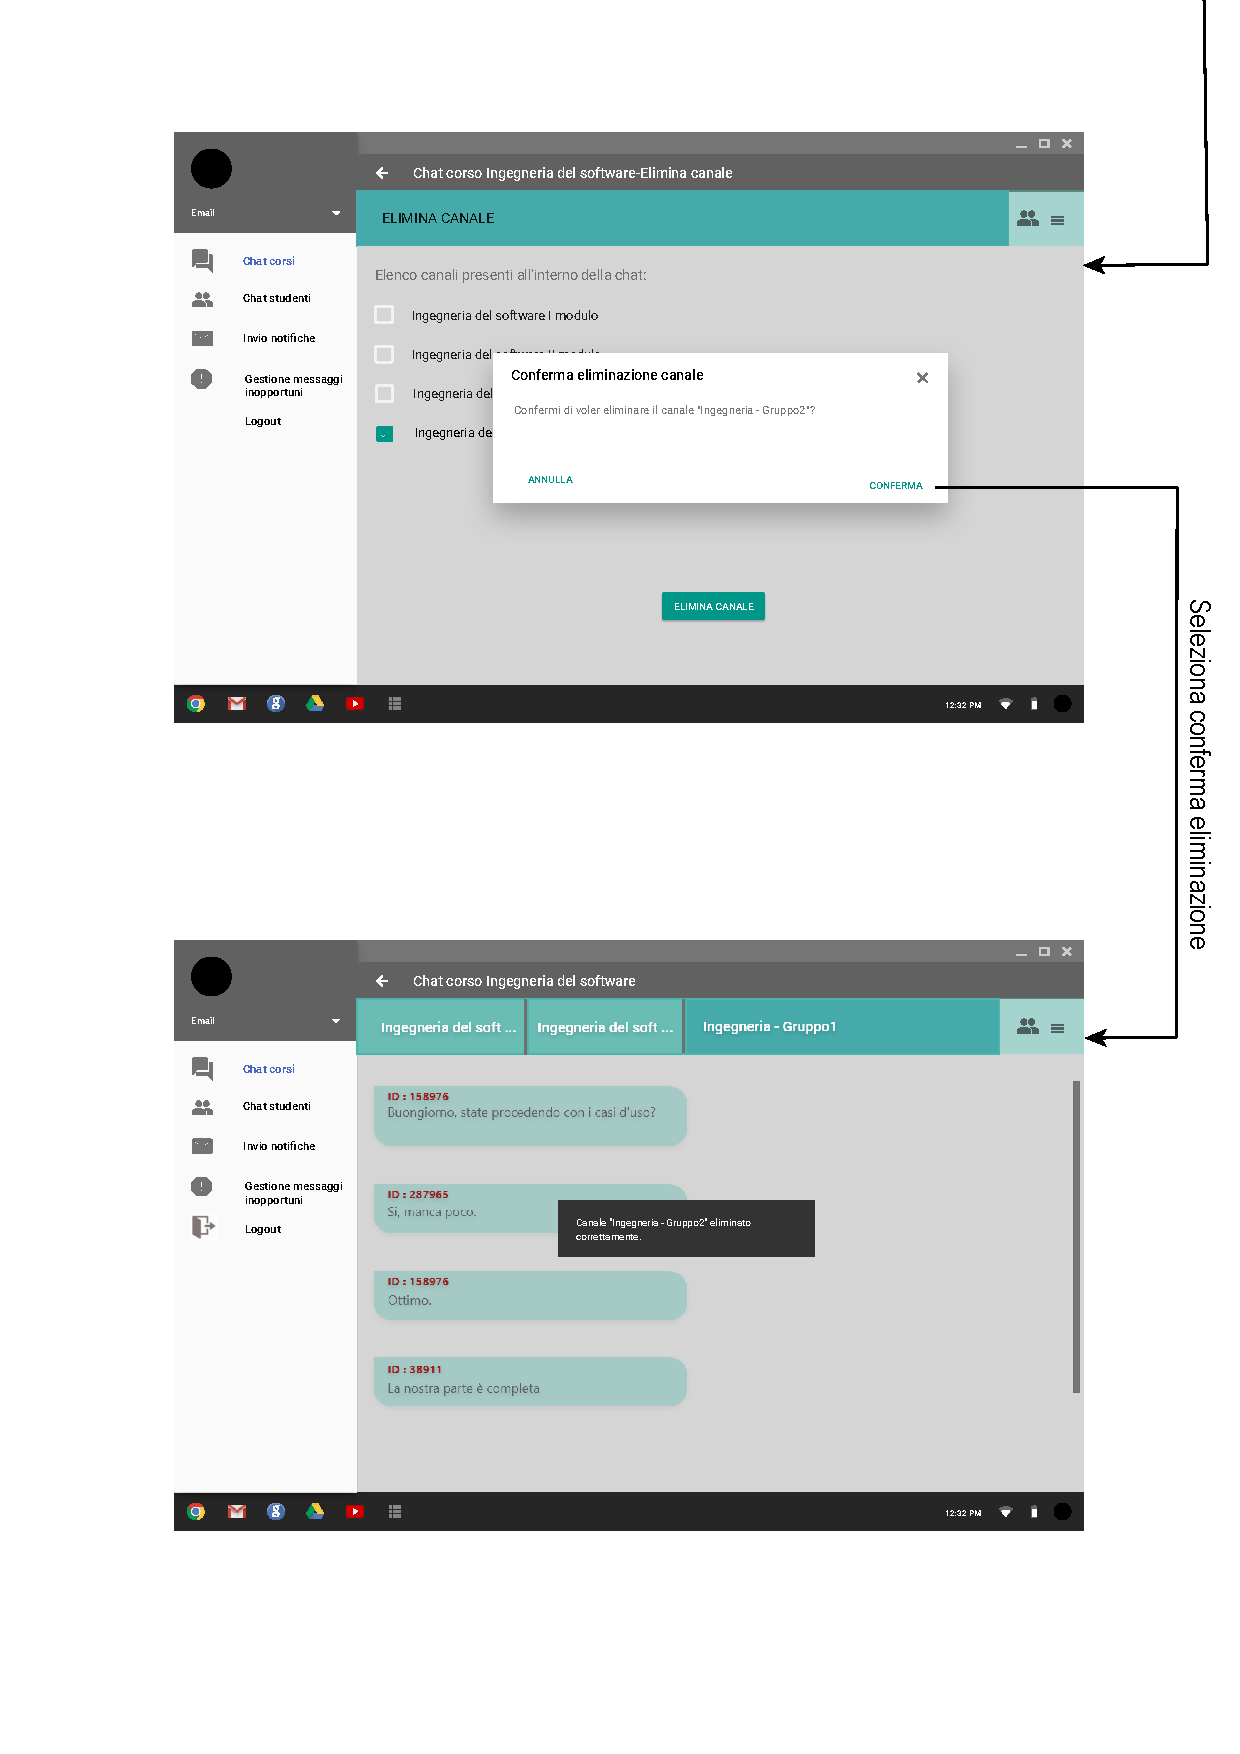
\includegraphics[width=0.9\textwidth]{imgs/gruppo6/activities/act_cup9_cancella_canale2.pdf}
	\caption{CUP9 - Cancella canale (pt.2)}
	\label{fig:cup9-2}
\end{figure}

\begin{figure}
	\centering
	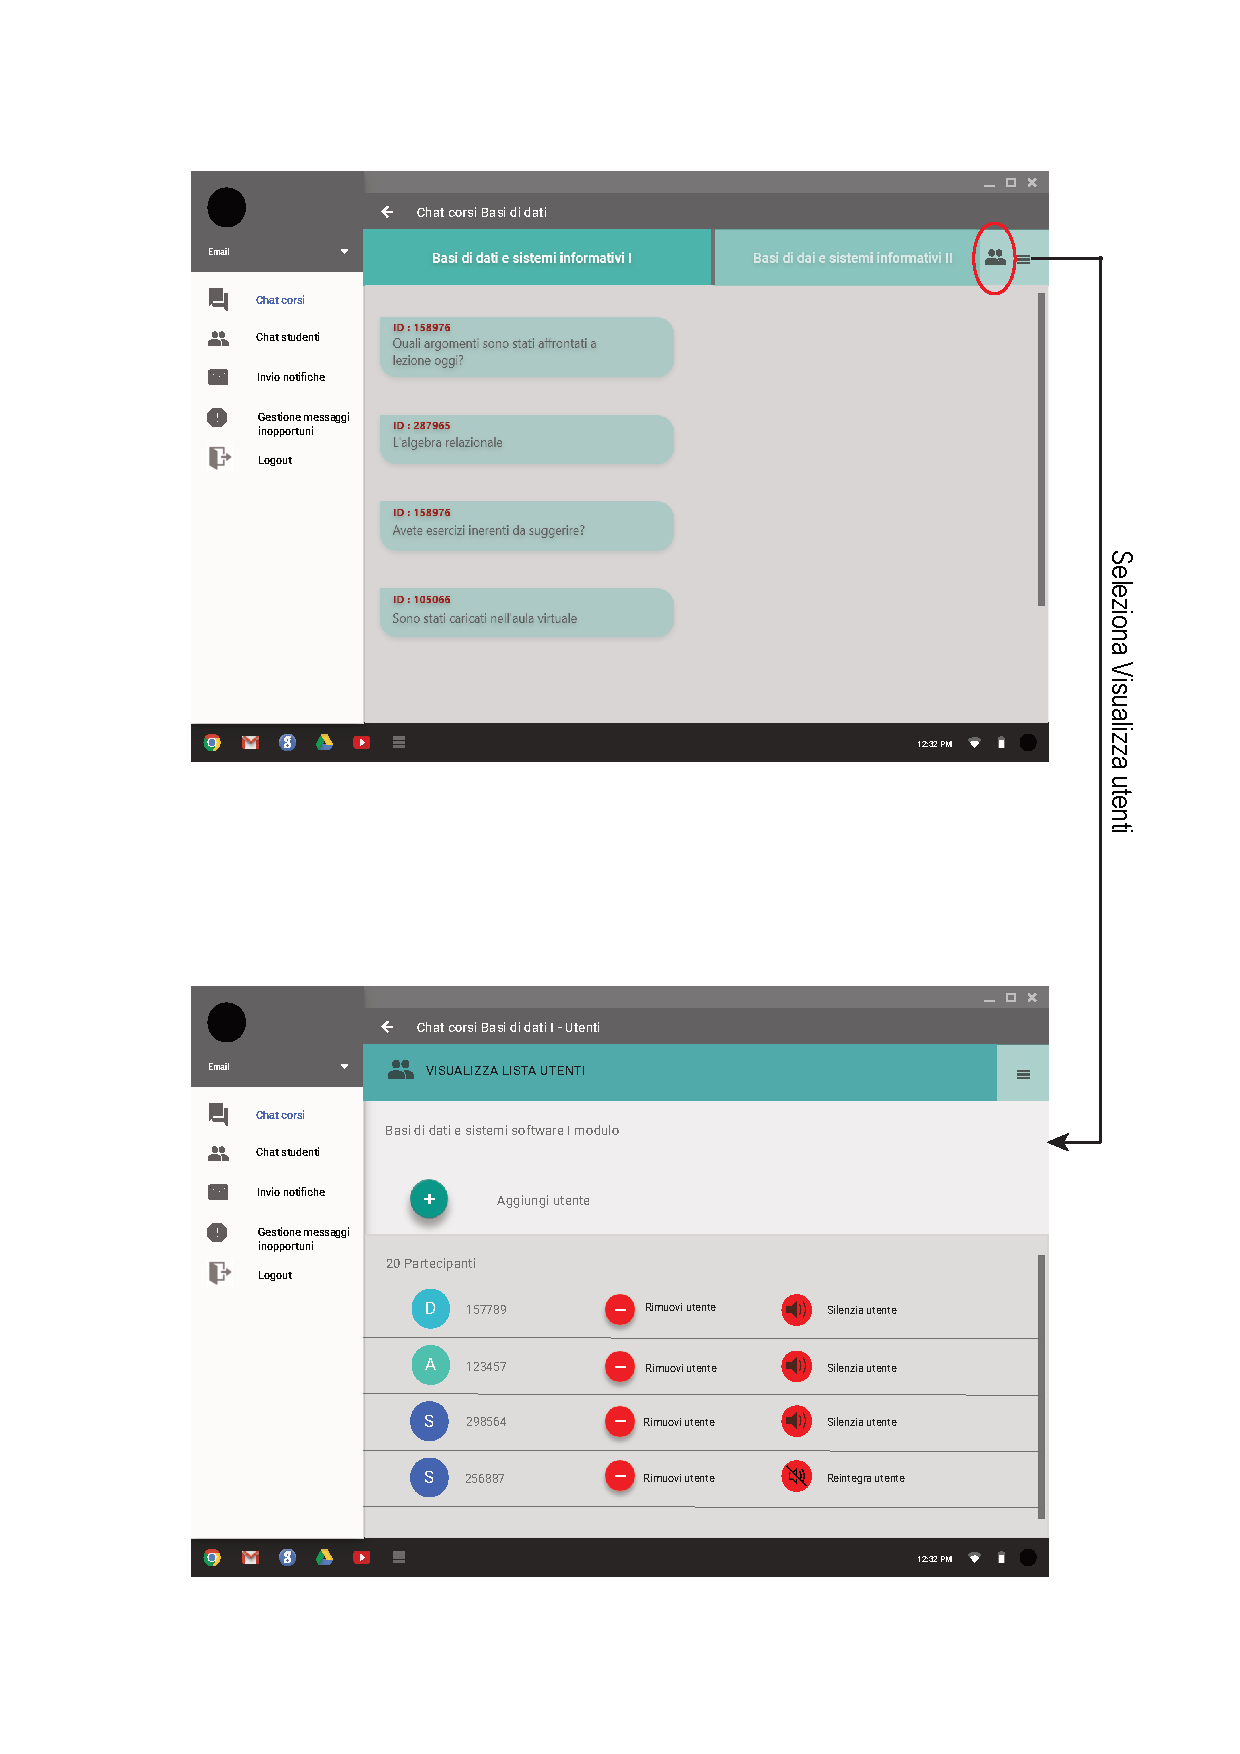
\includegraphics[width=0.9\textwidth]{imgs/gruppo6/activities/act_cup10_visualizza_lista_utenti.pdf}
	\caption{CUP10 - Visualizza lista utenti}
	\label{fig:cup10}
\end{figure}

\begin{figure}
	\centering
	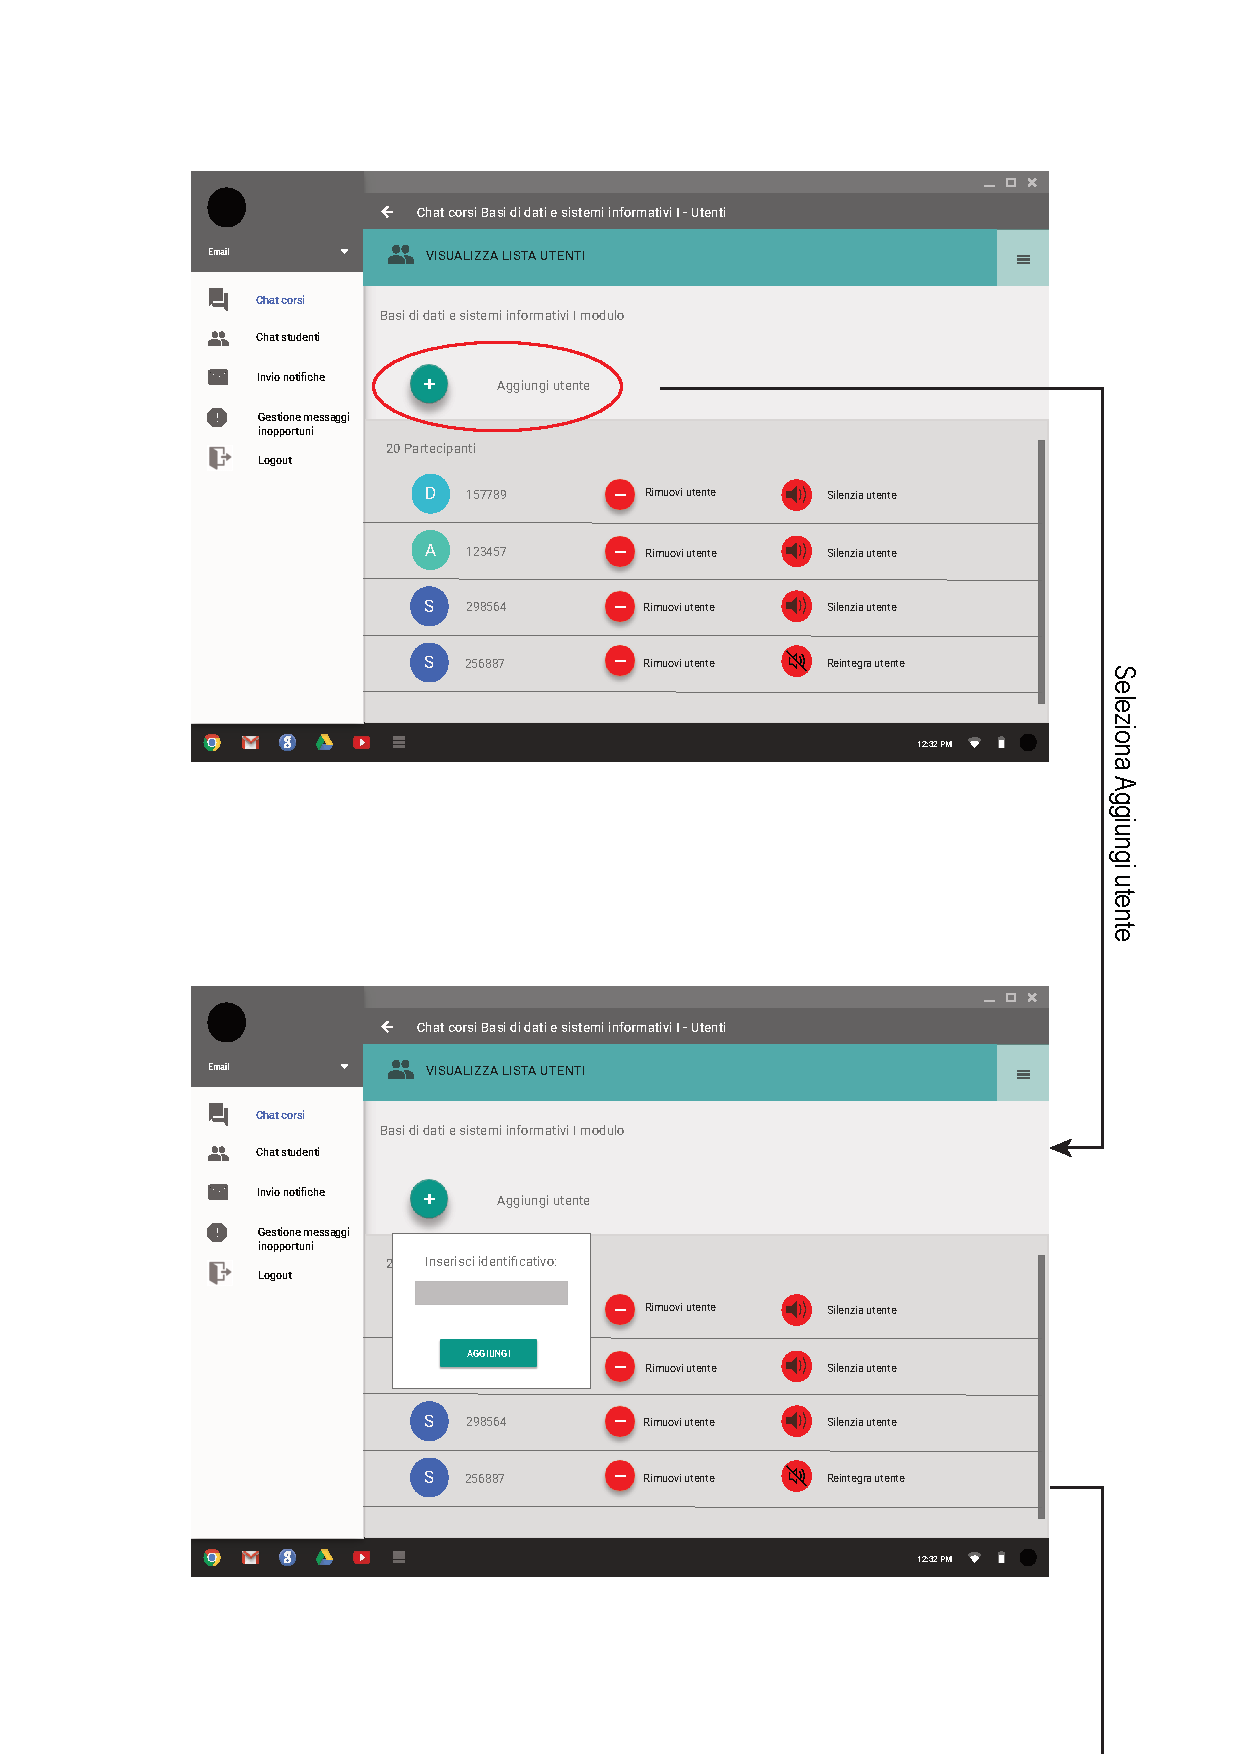
\includegraphics[width=0.9\textwidth]{imgs/gruppo6/activities/act_cup11_aggiungi_utente_canale1.pdf}
	\caption{CUP11 - Aggiungi un utente ad un canale (pt.1)}
	\label{fig:cup11}
\end{figure}

\begin{figure}
	\centering
	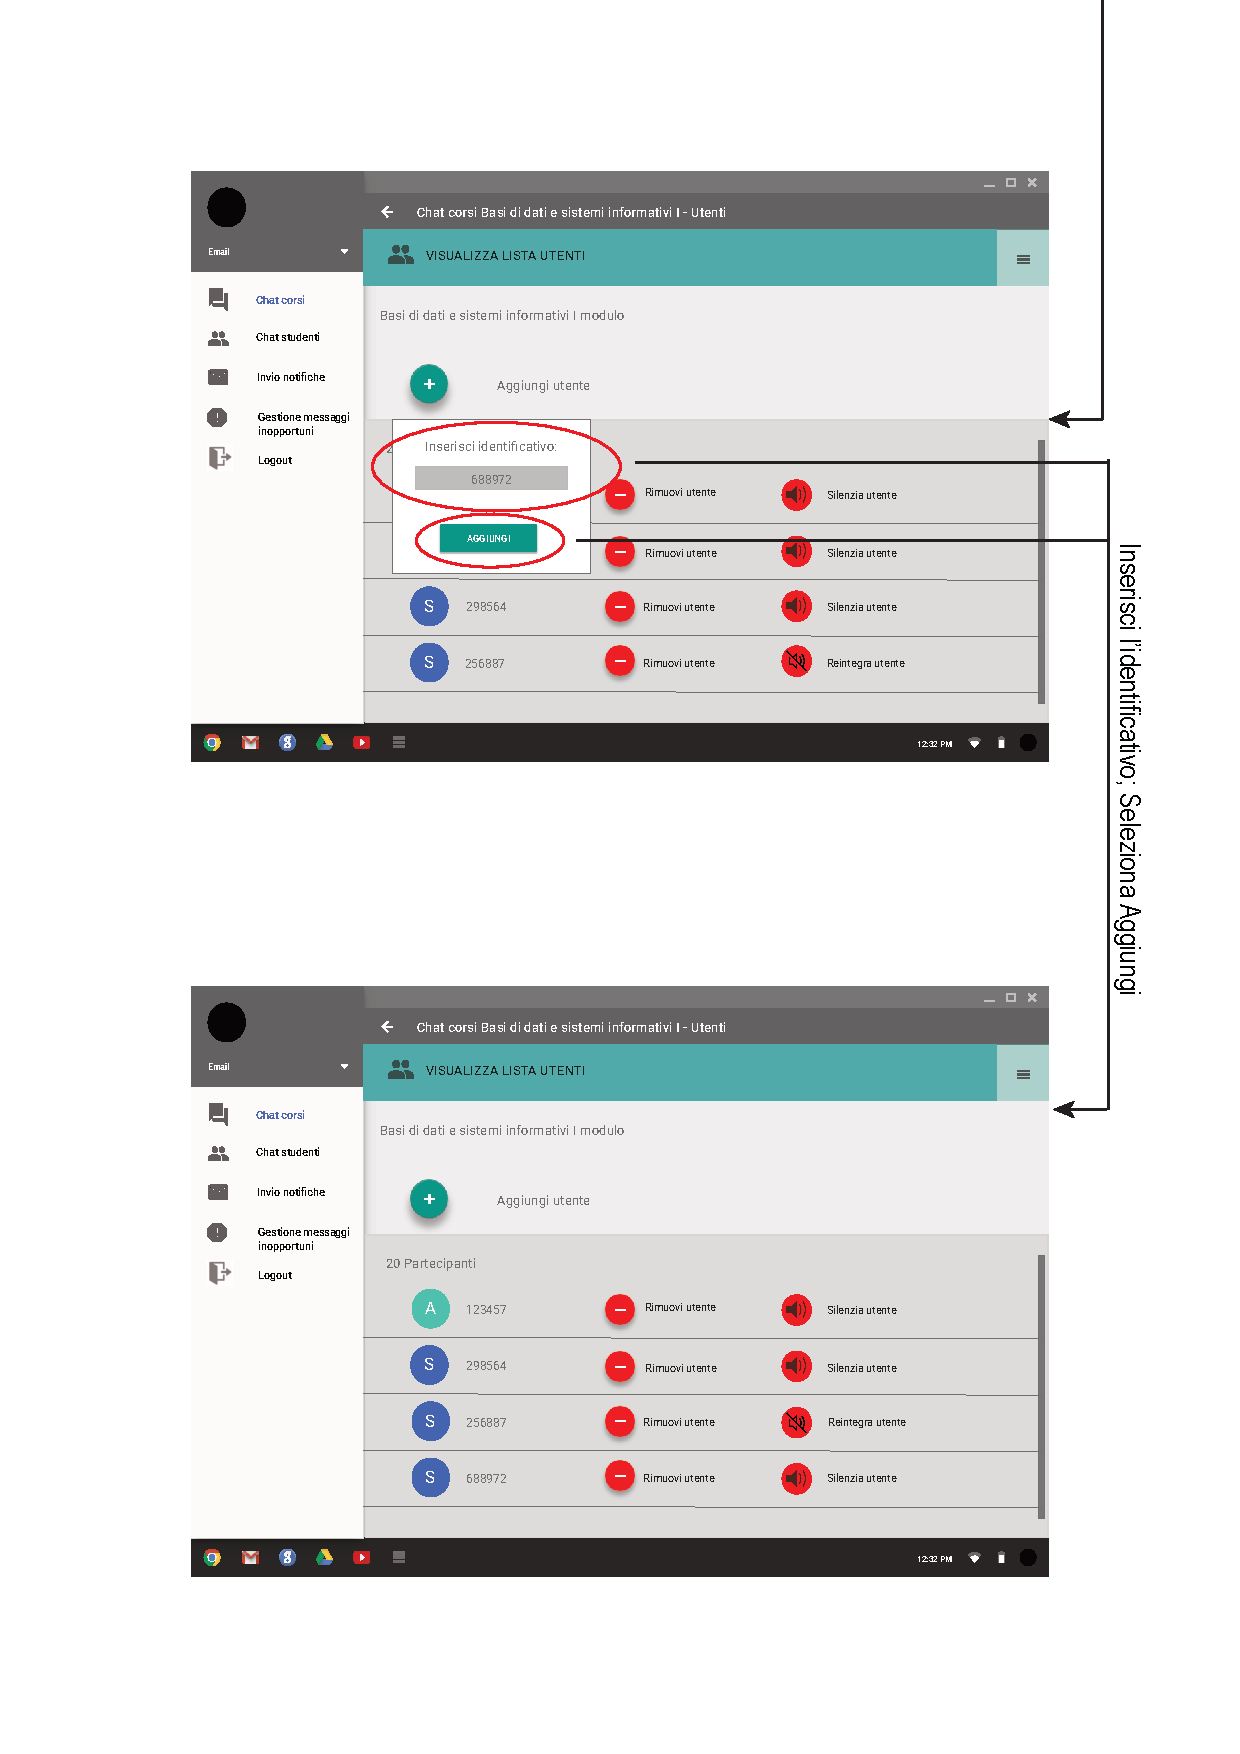
\includegraphics[width=0.9\textwidth]{imgs/gruppo6/activities/act_cup11_aggiungi_utente_canale2.pdf}
	\caption{CUP11 - Aggiungi un utente ad un canale (pt.2)}
	\label{fig:cup11-2}
\end{figure}

\begin{figure}
	\centering
	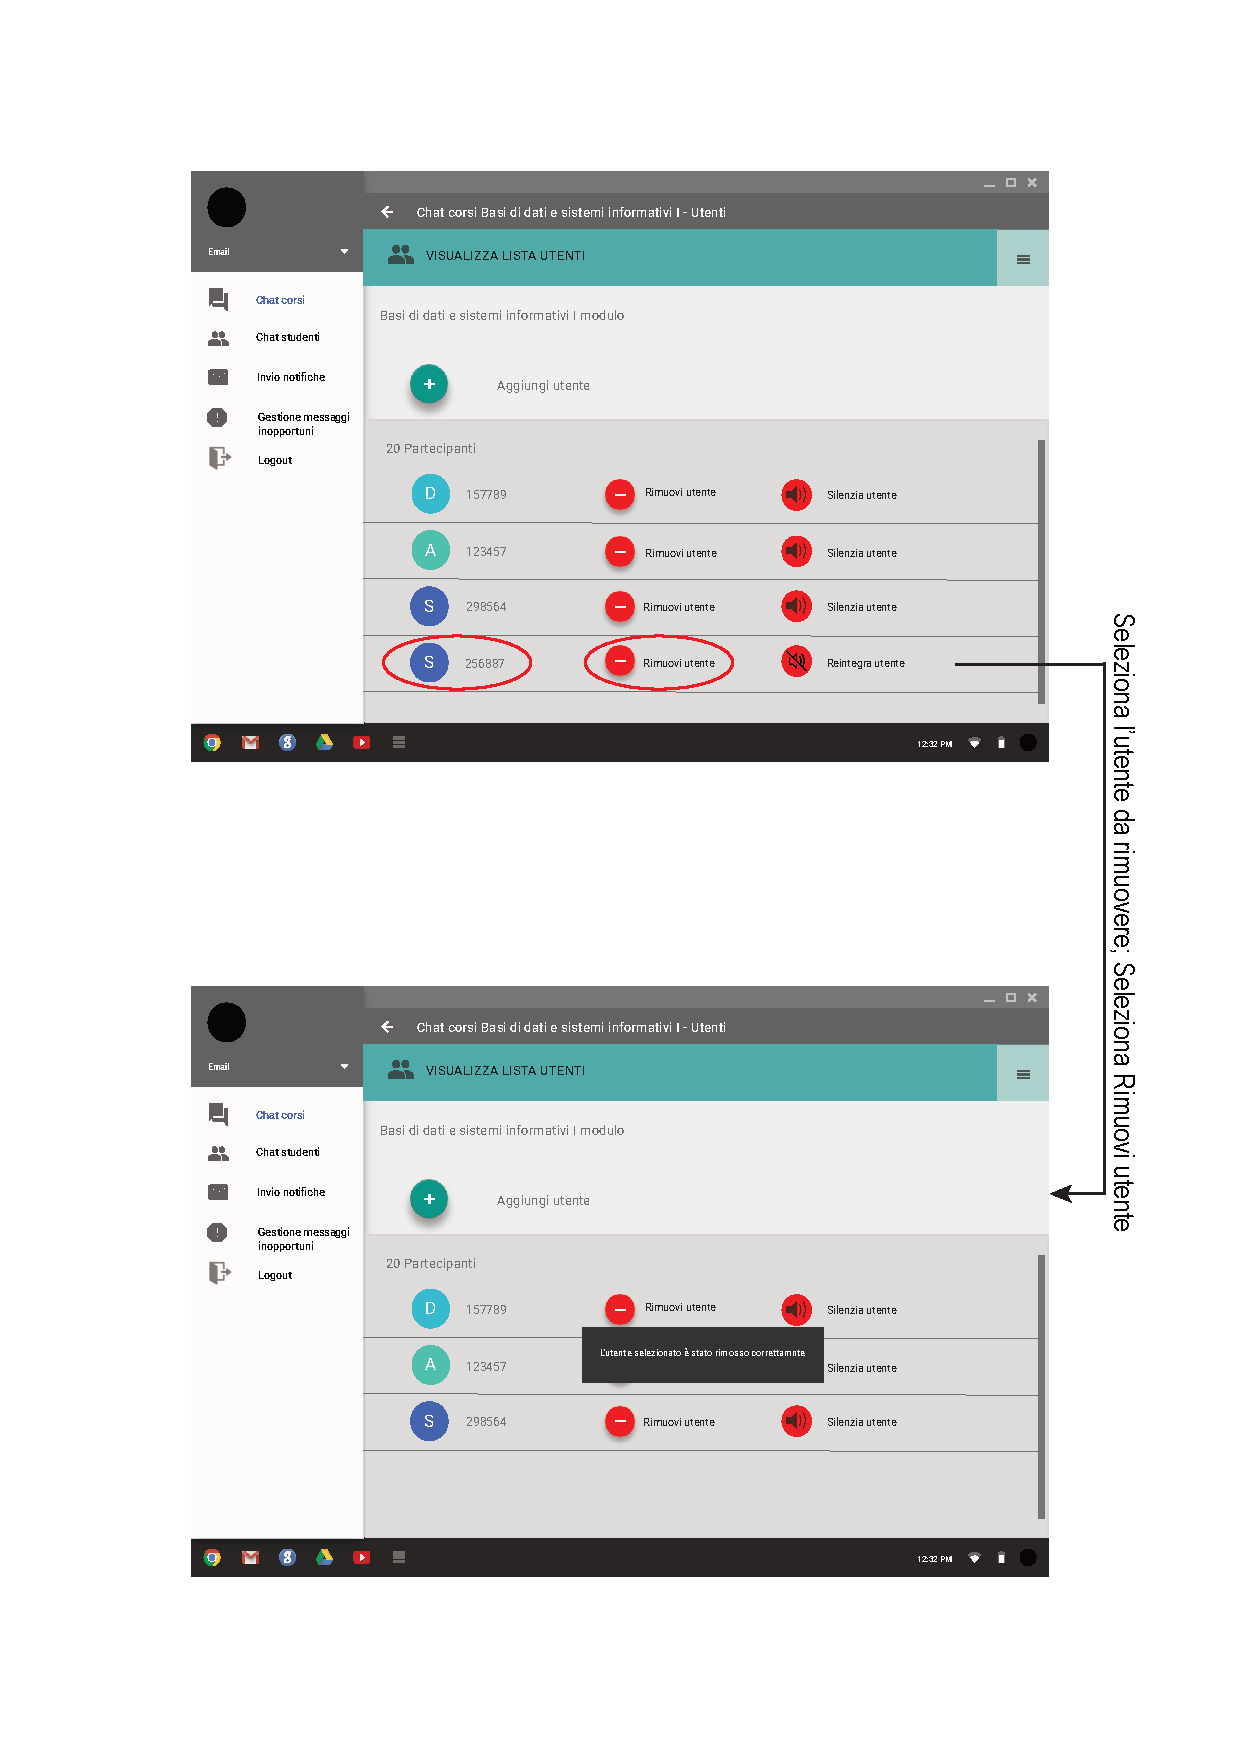
\includegraphics[width=0.9\textwidth]{imgs/gruppo6/activities/act_cup12_cancella_utente_canale.pdf}
	\caption{CUP12 - Rimuovere un utente da un canale}
	\label{fig:cup12}
\end{figure}

\begin{figure}
	\centering
	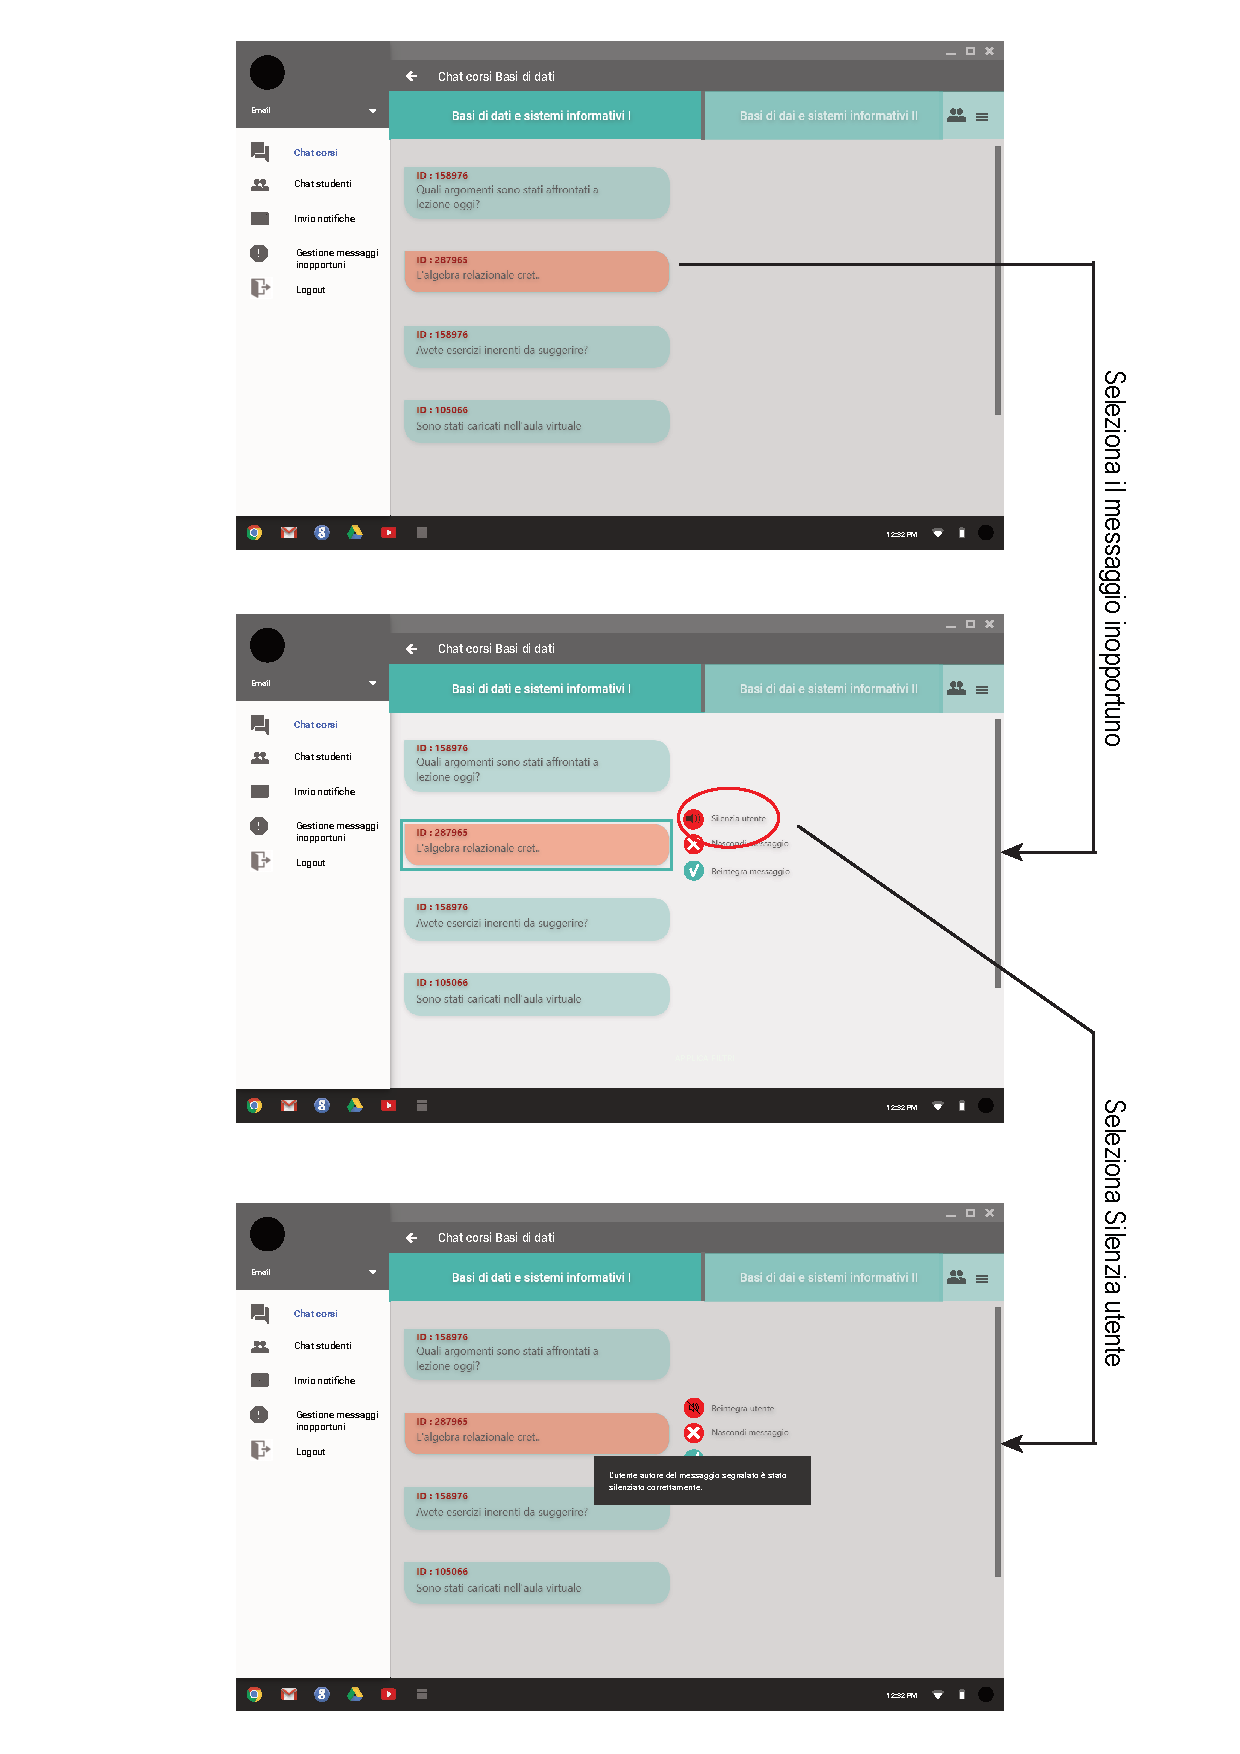
\includegraphics[width=0.9\textwidth]{imgs/gruppo6/activities/act_cup13_silenziare_utente1.pdf}
	\caption{CUP13 - Silenziare utente in un canale (pt.1)}
	\label{fig:cup13}
\end{figure}

\begin{figure}
	\centering
	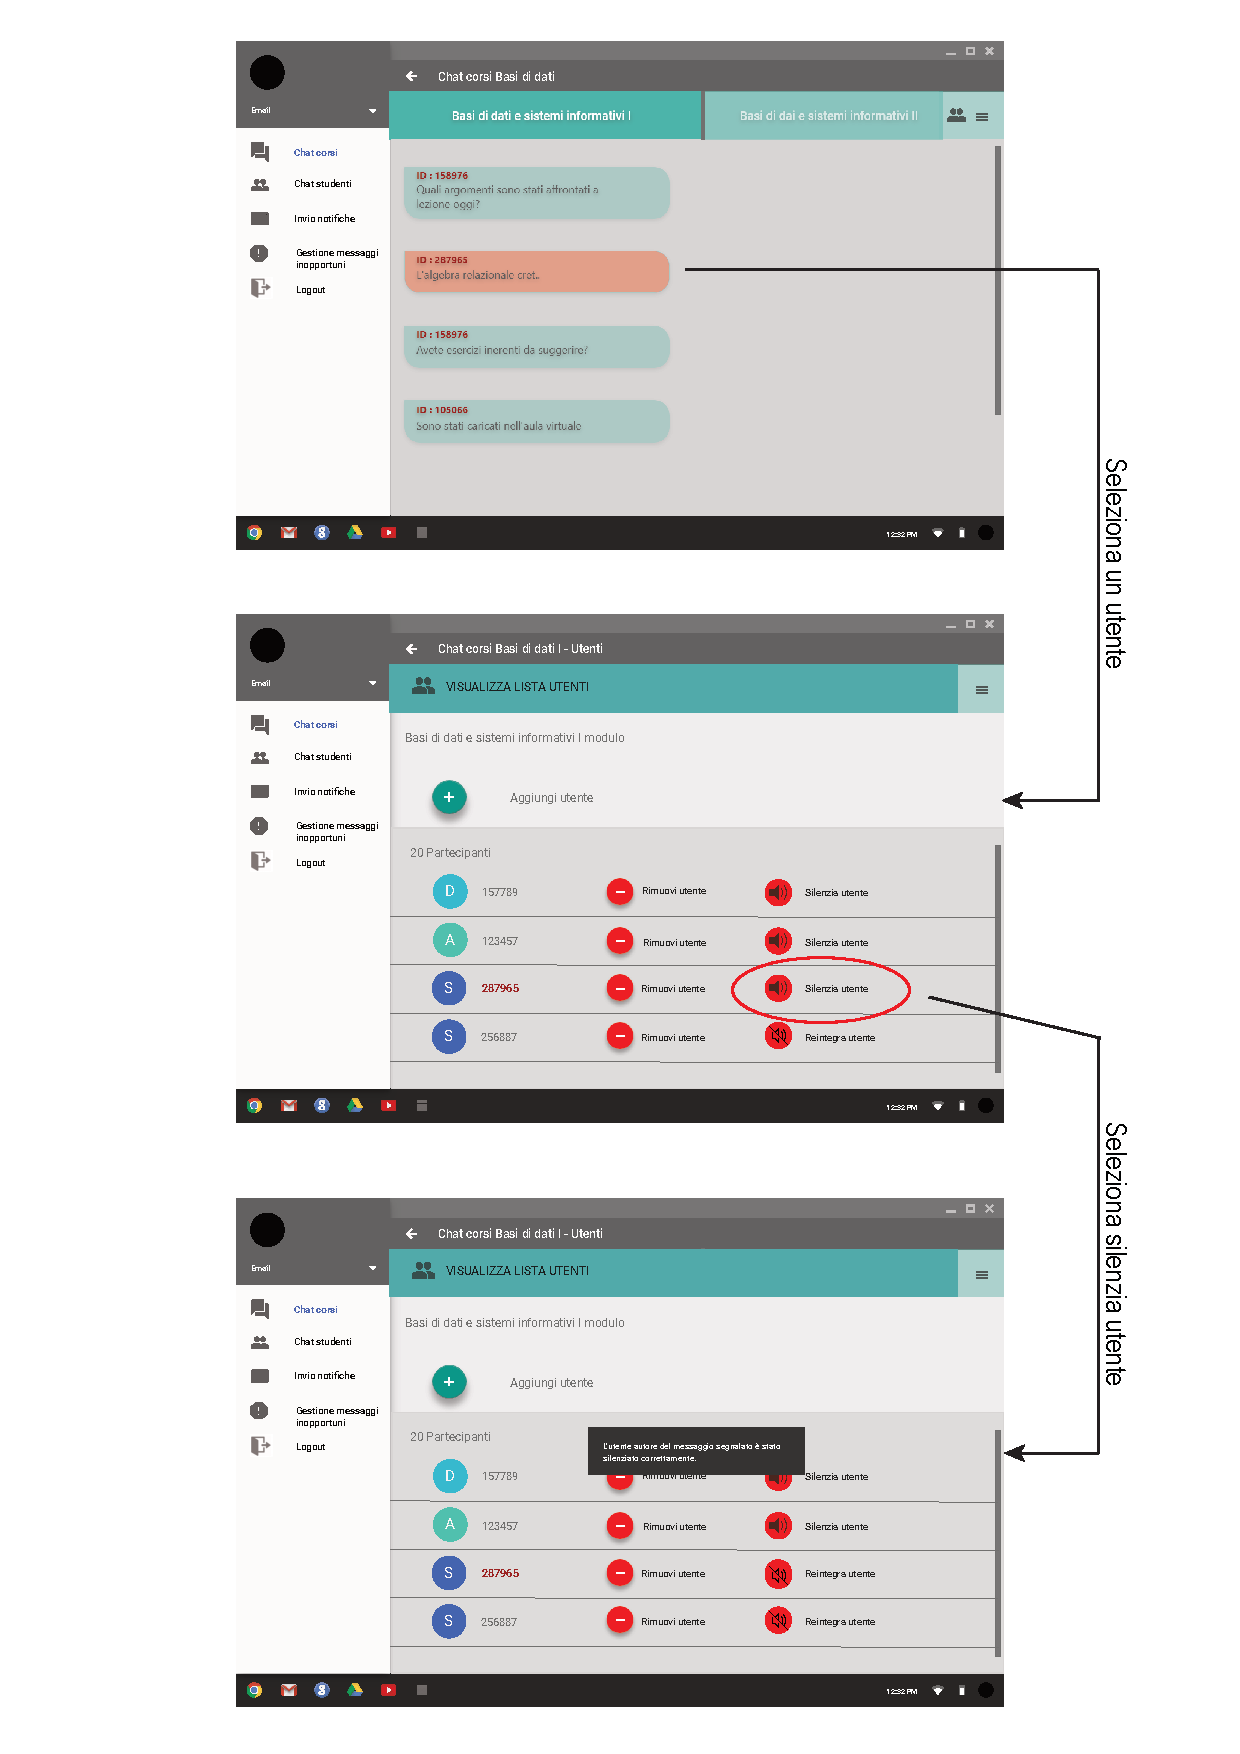
\includegraphics[width=0.9\textwidth]{imgs/gruppo6/activities/act_cup13_silenziare_utente2.pdf}
	\caption{CUP13 - Silenziare utente in un canale (pt.2)}
	\label{fig:cup13-2}
\end{figure}

\begin{figure}
	\centering
	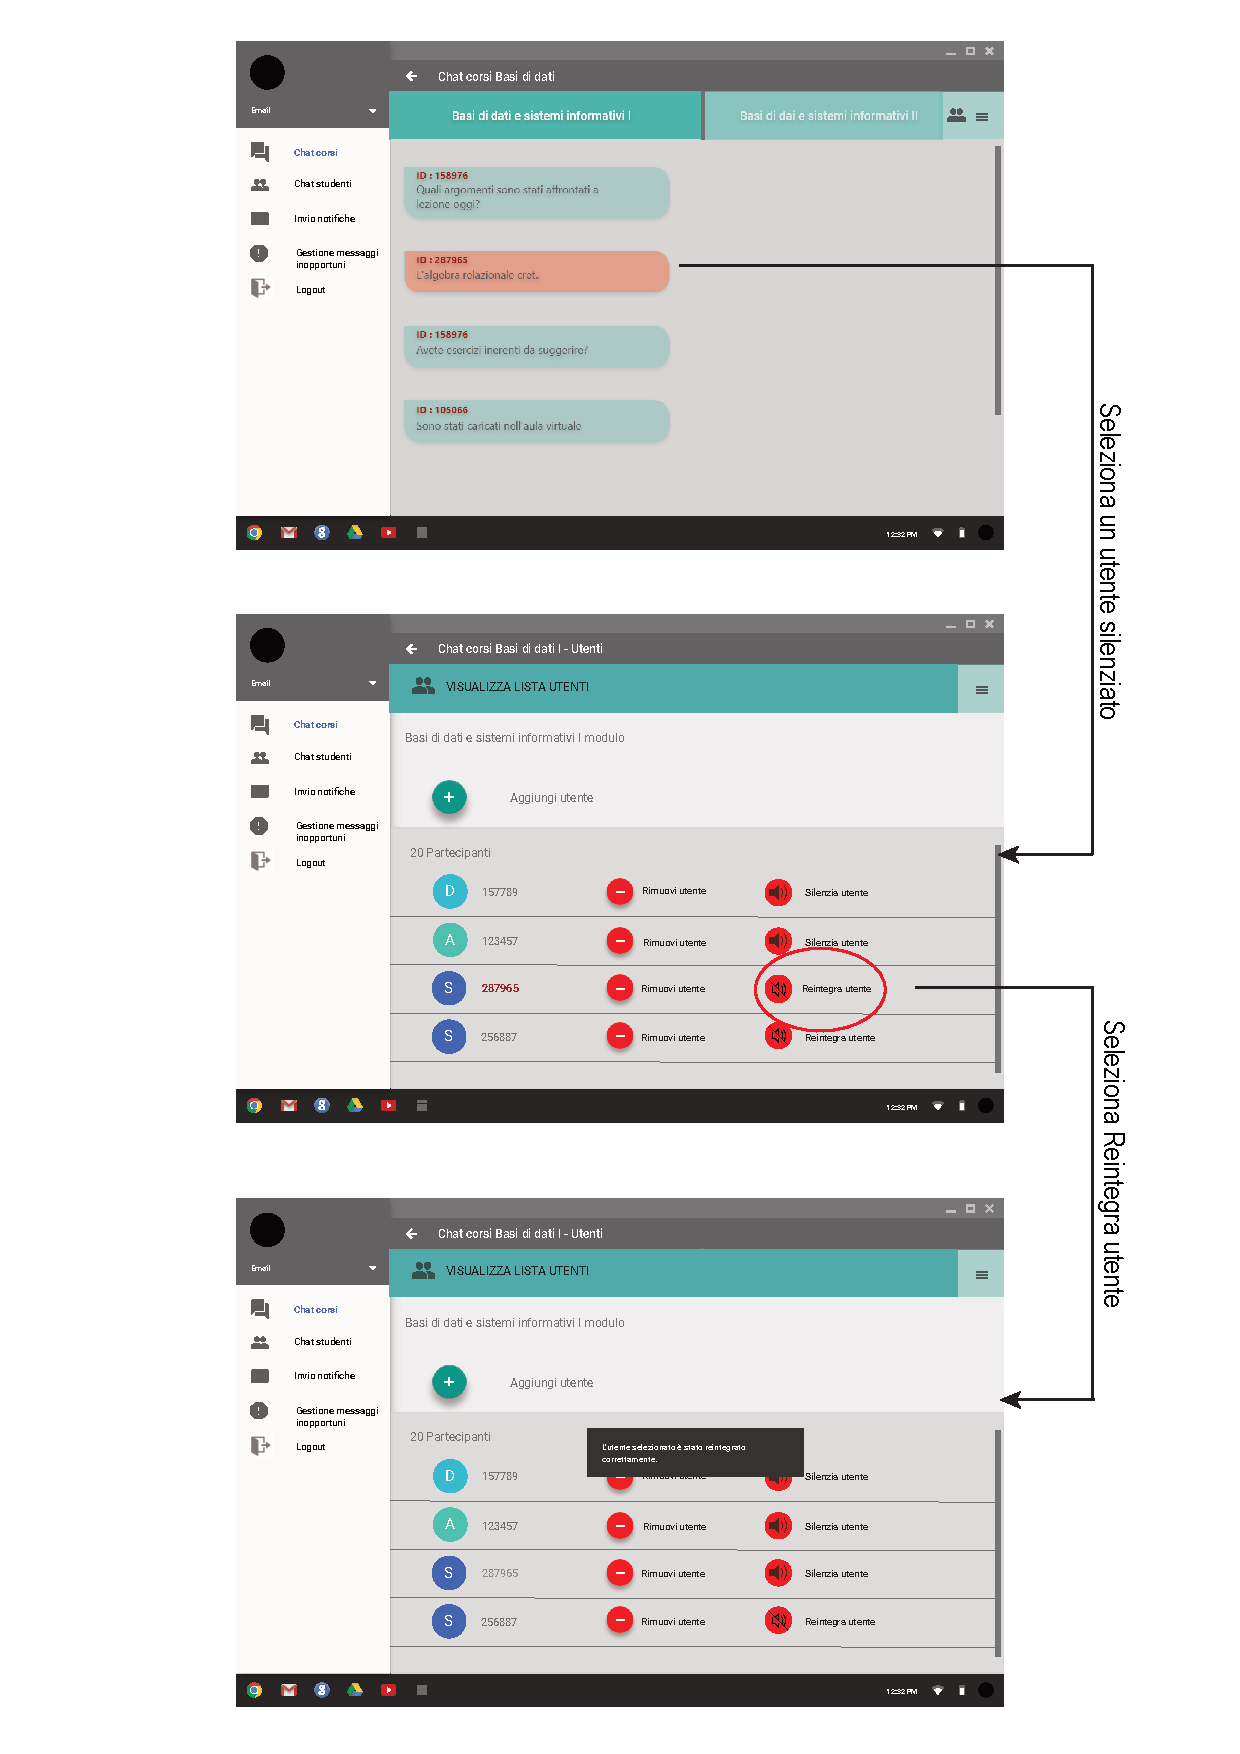
\includegraphics[width=0.9\textwidth]{imgs/gruppo6/activities/act_cup14_reintegra_utente.pdf}
	\caption{CUP14 - Reintegra utente in un canale}
	\label{fig:cup14}
\end{figure}

\begin{figure}
	\centering
	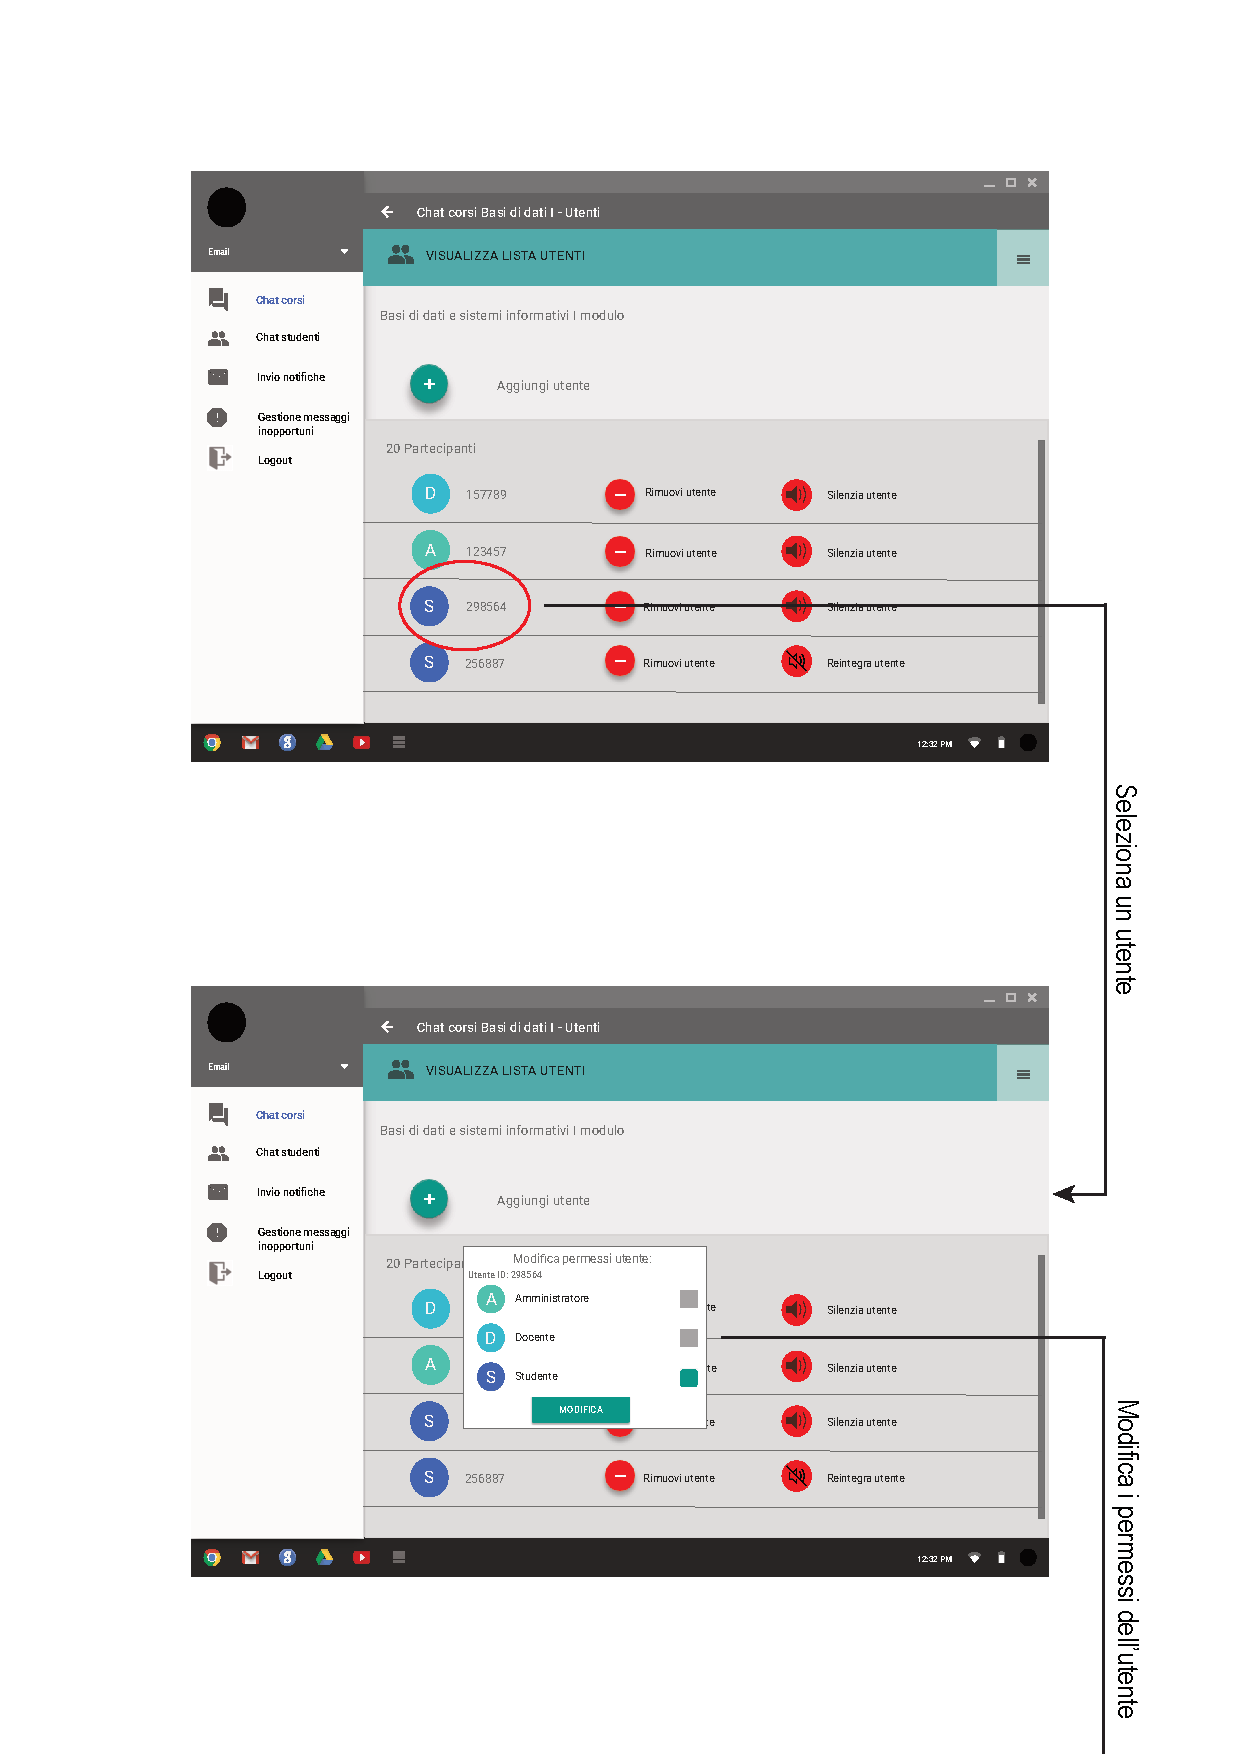
\includegraphics[width=0.9\textwidth]{imgs/gruppo6/activities/act_cup15_modifica_permessi_utente1.pdf}
	\caption{CUP15 - Modificare i permessi di un utente in un canale (pt.1)}
	\label{fig:cup15-2}
\end{figure}

\begin{figure}
	\centering
	\includegraphics[width=0.9\textwidth]{imgs/gruppo6/activities/act_cup15_modifica_permessi_utente2.pdf}
	\caption{CUP15 - Modificare i permessi di un utente in un canale (pt.2)}
	\label{fig:cup15-2}
\end{figure}

\begin{figure}
	\centering
	\includegraphics[width=0.9\textwidth]{imgs/gruppo6/activities/act_cup16_nascondi_messaggio.pdf}
	\caption{CUP16 - Nascondi messaggio}
	\label{fig:cup16}
\end{figure}

\begin{figure}
	\centering
	\includegraphics[width=0.9\textwidth]{imgs/gruppo6/activities/act_cup17_reintegra_messaggio.pdf}
	\caption{CUP17  - Reintegra messaggio}
	\label{fig:cup17}
\end{figure}

\begin{figure}
	\centering
	\includegraphics[width=0.9\textwidth]{imgs/gruppo6/activities/act_cup18_invio_notifiche1.pdf}
	\caption{CUP18 - Invio Notifiche (pt.1)}
	\label{fig:cup18}
\end{figure}

\begin{figure}
	\centering
	\includegraphics[width=0.9\textwidth]{imgs/gruppo6/activities/act_cup18_invio_notifiche2.pdf}
	\caption{CUP18 - Invio Notifiche (pt.2)}
	\label{fig:cup18-2}
\end{figure}

\begin{figure}
	\centering
	\includegraphics[width=0.9\textwidth]{imgs/gruppo6/activities/act_cup19_gestione_messaggi_inopportuni.pdf}
	\caption{CUP19 - Gestione messaggi inopportuni}
	\label{fig:cup19}
\end{figure}
%%% END activities chat pannello %%%
\clearpage